\chapter{Celda Sedra-Ghorab-Martin (R)}

\section{Introducción}
En un paper presente en el volumen 12 de la publicación IEEE Transactions on Circuits and Systems, de diciembre de 1980, A. Sedra, M. Ghorab y K. Martin propusieron dos circuitos bicuadráticos (con funciones transferencia de denominador y numerador de orden dos) que hacen uso de la estructura de retroalimentación positiva de Sallen-Key. 

\begin{figure}[H]
\begin{centering}
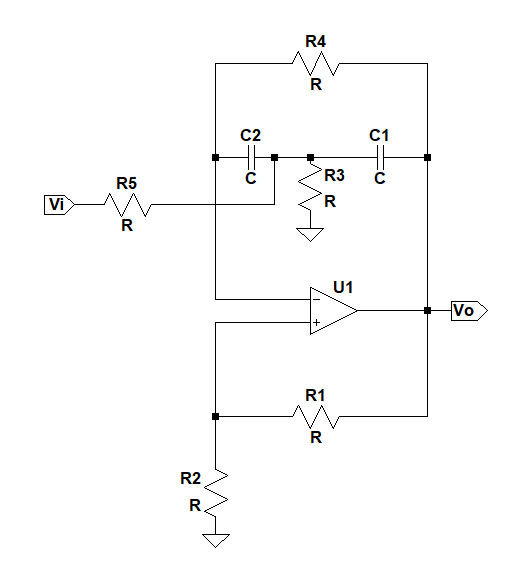
\includegraphics[width=0.4\textwidth]{../Ex3/Resources/Deliyannis}
\par\end{centering}
\caption{Circuito Pasabanda Deliyannis}
\label{3_1}
\end{figure}

Estos circuitos tienen sensibilidades y ecuaciones de diseño de polos idénticas al circuito de Deliyannis, que es la base del filtro Deliyannis-Friend. Sin embargo, mejoran las sensibilidades de los ceros de transmisión, además de permitir el diseño de todos los tipos posibles de filtros de segundo orden.

En la presente sección, se hace uso del circuito propuesto en esa publicación para implementar cada una de las etapas de un filtro a partir de una plantilla propuesta por la cátedra.

\section{Marco teórico} \label{marcoteorico}
Se parte del circuito pasa-banda propuesto por Deliyannis que se muestra en la
Figura \ref{3_1}. Este circuito fue modificado por Friend, cargando la T, para poder implementar otras funciones de filtros. Sin embargo, el circuito resultante no puede ser utilizado para implementar un filtro pasa-bajos, además de tener un proceso de diseño trabajoso.

Los autores de la publicación plantean como alternativa realizar la transformación complementaria del circuito, que resultará en la estructura de retroalimentación positiva de Sallen-Key y además preservará los polos del circuito original y sus sensibilidades.

En la Figura \ref{salkey} se pueden observar el circuito de Deliyannis (a), una variante (c), y sus transformaciones complementarias (b y d, respectivamente). La transformación complementaria involucra aterrar todo aquello que esté conectado a la salida del op-amp, conectar lo que esté a tierra a la salida del op-amp, e invertir las entradas del op-amp.

\begin{figure}[H]
\begin{centering}
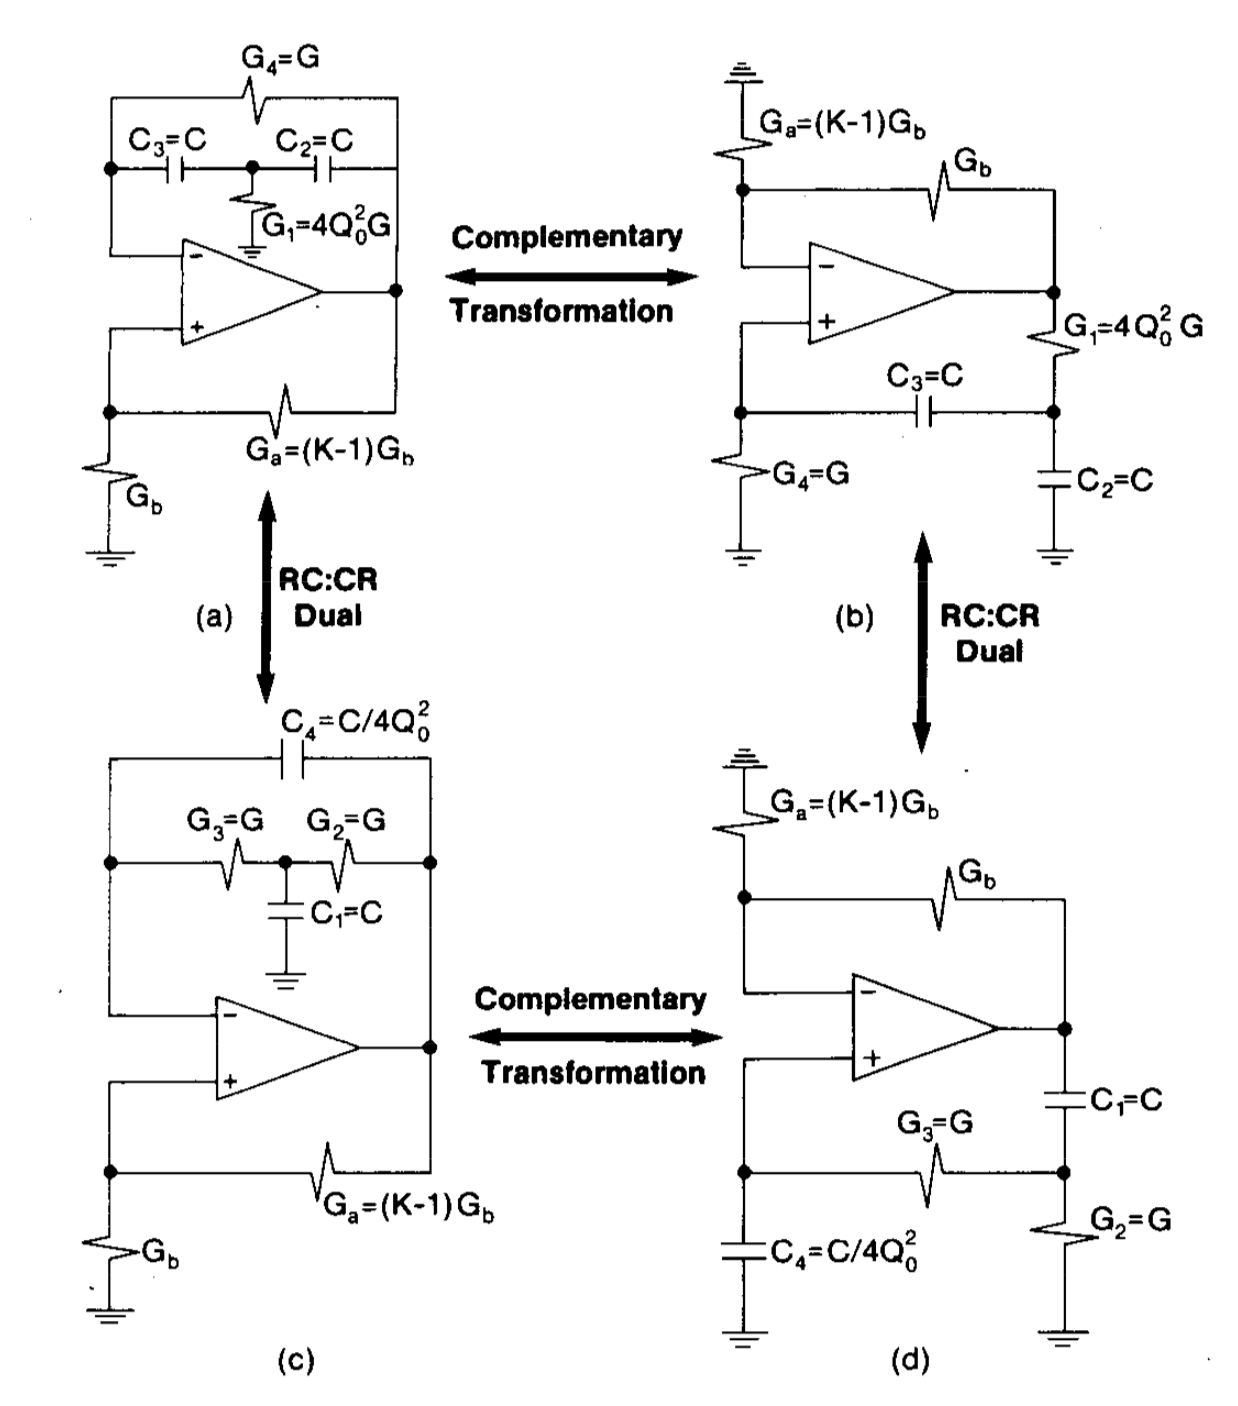
\includegraphics[width=0.4\textwidth]{../Ex3/Resources/sallenkeystructures.png}
\par\end{centering}
\caption{Transformaciones complementarias de los circuitos de Deliyannis}
\label{salkey}
\end{figure}

Para implementar mediante los circuitos (b) y (d) de la Figura \ref{salkey} todos los tipos de filtro, se le deben agregar ceros de transmisión de forma tal que cumplan una función transferencia de la forma 
\begin{equation*}
    T(s)=\frac{n_{2}s^2+n_{1}s+n_{0}}{s^2+s(\frac{\omega_{0}}{Q})+\omega_{0}^2}
\end{equation*}
donde $n_{2}$, $n_{1}$ y $n_{0}$ son coeficientes que determinan los ceros de transmisión y que dependerán del tipo de filtro a implementar.

Es aquí que se encuentra la clave del descubrimiento: para implementar la función transferencia con estos circuitos sin modificar sus polos ni las sensibilidades de los mismos, se propone desaterrar de forma completa o parcial todos los componentes que previamente estaban a tierra, y conectarlos a la fuente de señal de entrada. Los circuitos resultantes se pueden observar en la Figura \ref{sedracircs}. Aquí, el circuito (a) es el pasa-altos bicuadrático (HPB, por sus siglas en inglés), y el (b) es el pasa-bajos bicuadrático (LPB). Están basados en los circuitos (b) y (d) de la Figura \ref{salkey}, respectivamente.


\begin{figure}[H]
\begin{centering}
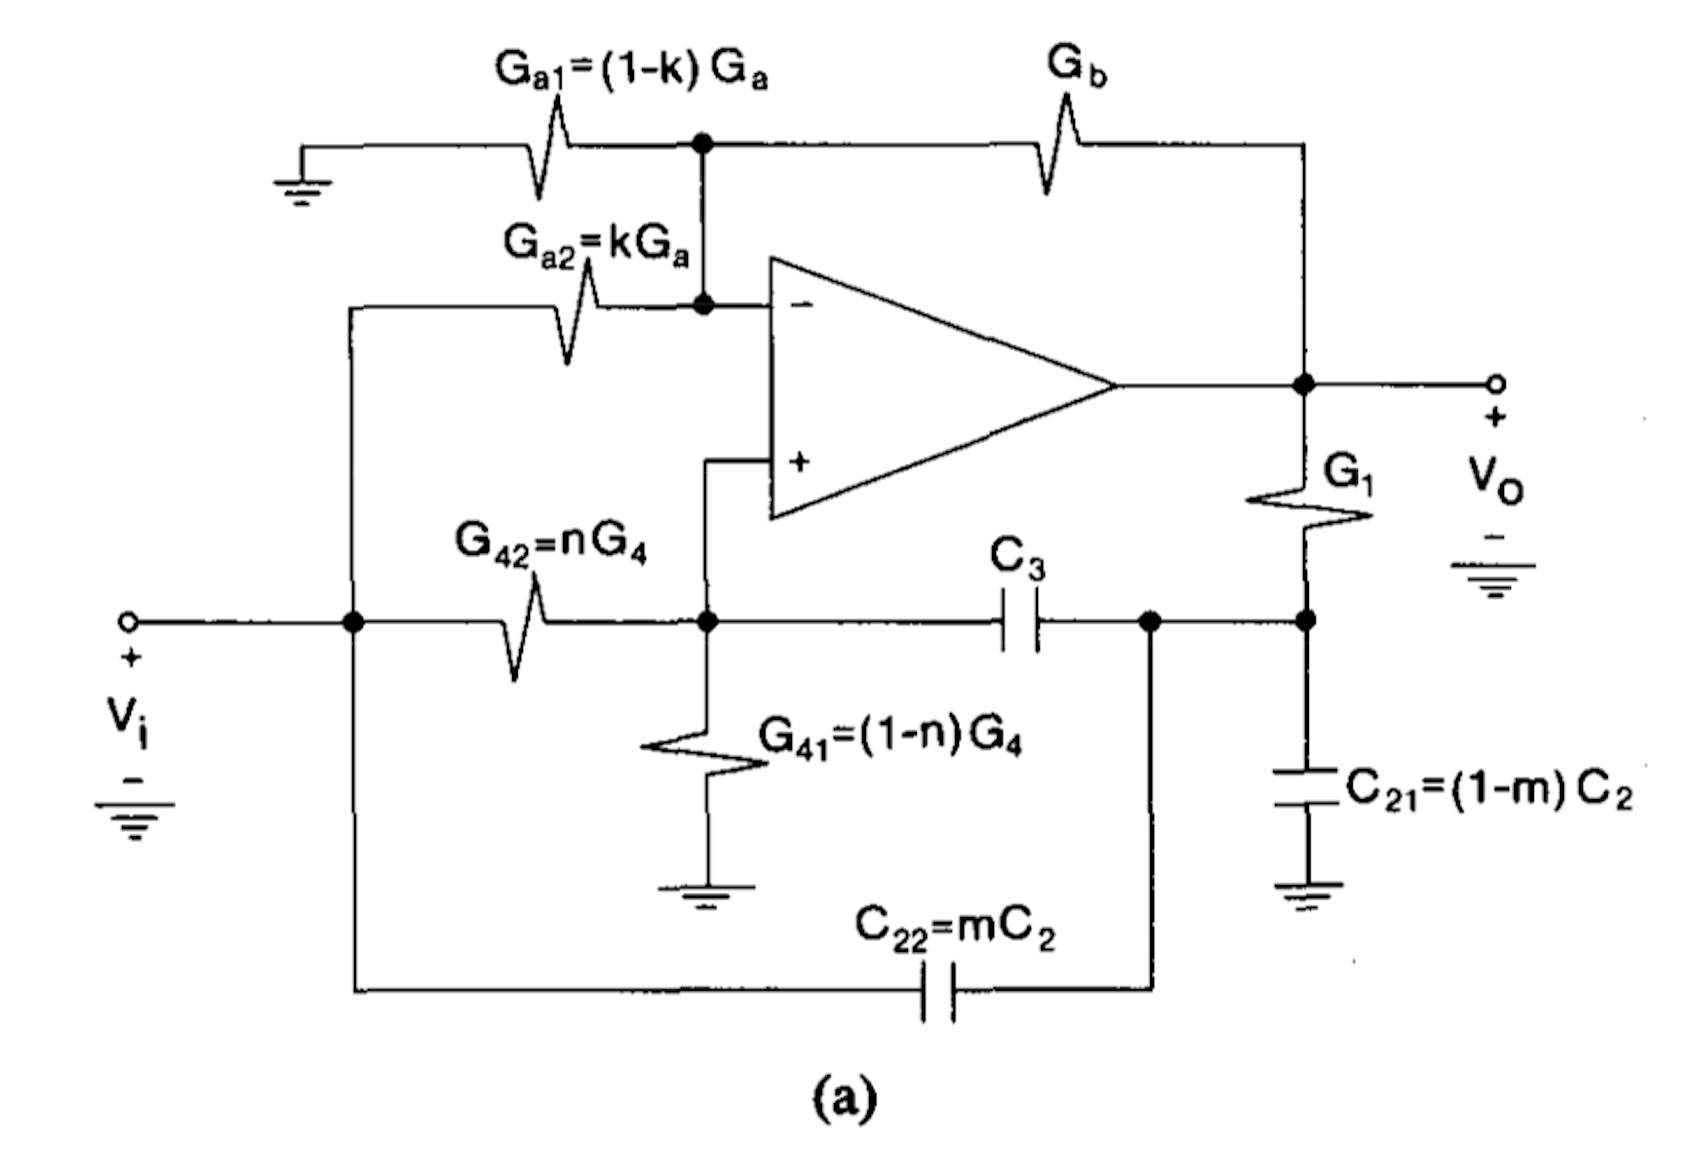
\includegraphics[width=0.45\textwidth]{../Ex3/Resources/sedracirc1.png}
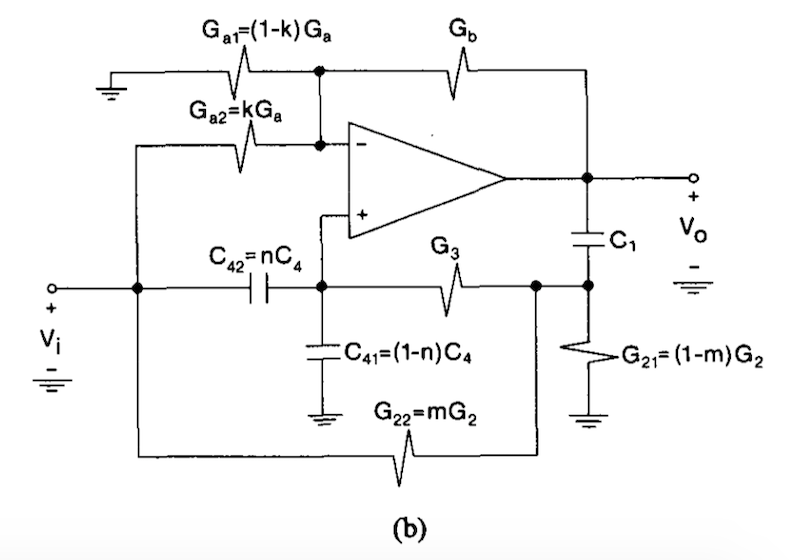
\includegraphics[width=0.45\textwidth]{../Ex3/Resources/sedracirc2.png}
\par\end{centering}
\caption{Circuitos HPB y LPB propuestos por los autores}
\label{sedracircs}
\end{figure}

Resolviendo el circuito, se obtiene la función transferencia que debe ajustarse a la plantilla. A partir de esta se deducen los valores de los componentes, se realiza un análisis de sensibilidades y se procede a diseñar el filtro.




\section{Diseño}
\subsection{Aproximación del filtro}
Se eligió una plantilla más restrictiva que la propuesta por la cátedra (Cuadro \ref{3_c_1}) para disponer de un margen razonable de error. La plantilla se ve en el Cuadro \ref{plantrestrictiva}. 

\begin{table}[H]
\begin{centering}
\begin{tabular}{|c|c|}
\hline 
 & Frecuencia\tabularnewline
\hline 
\hline 
$f_{a}$ & 12.2 (kHz)\tabularnewline
\hline 
$f_{p}$ & 24.4 (kHz)\tabularnewline
\hline 
$A_{a}$ & 40 dB\tabularnewline
\hline 
$A_{p}$ & 2 dB\tabularnewline
\hline 
$\left|Z_{in}(f)\right|$ & $\geq50\,(k\Omega)$\tabularnewline
\hline 
\end{tabular}
\par\end{centering}
\caption{Plantilla del filtro propuesto por la cátedra}
\label{3_c_1}
\end{table}

\begin{table}[H]
\begin{centering}
\begin{tabular}{|c|c|}
\hline 
 & Frecuencia\tabularnewline
\hline 
\hline 
$f_{a}$ & 13 (kHz)\tabularnewline
\hline 
$f_{p}$ & 23 (kHz)\tabularnewline
\hline 
$A_{a}$ & 45 dB\tabularnewline
\hline 
$A_{p}$ & 1 dB\tabularnewline
\hline 
$\left|Z_{in}(f)\right|$ & $\geq50\,(k\Omega)$\tabularnewline
\hline 
\end{tabular}
\par\end{centering}
\caption{Plantilla propuesta}
\label{plantrestrictiva}
\end{table}

En primer lugar, se debe escoger un método de aproximación para derivar de la plantilla  una función transferencia de un circuito que permita cumplir con los requerimentos de la misma: se eligió el método de aproximación de Cauer para obtener un orden mínimo y economizar en diseño y componentes.

Mediante cálculo simbólico asistido por computadora, se obtiene la siguiente función transferencia para la aproximación de Cauer de grado 4, que cumple con los requerimentos planteados:
\[
H(s)=\frac{891.2\cdot10^{-3}s^{4}+6.83\cdot10^{9}s^{2}+7.24\cdot10^{18}}{s^{4}+337,19\cdot10^{3}s^{3}+9.241\cdot10^{10}s^{2}+8.4\cdot10^{15}s+1.98\cdot10^{21}}
\]
La función transferencia y el diagrama de polos y ceros de esta aproximación pueden verse en las figuras \ref{bodecauer} y \ref{poloscauer}, respectivamente. 

\begin{figure}[H]
\begin{centering}
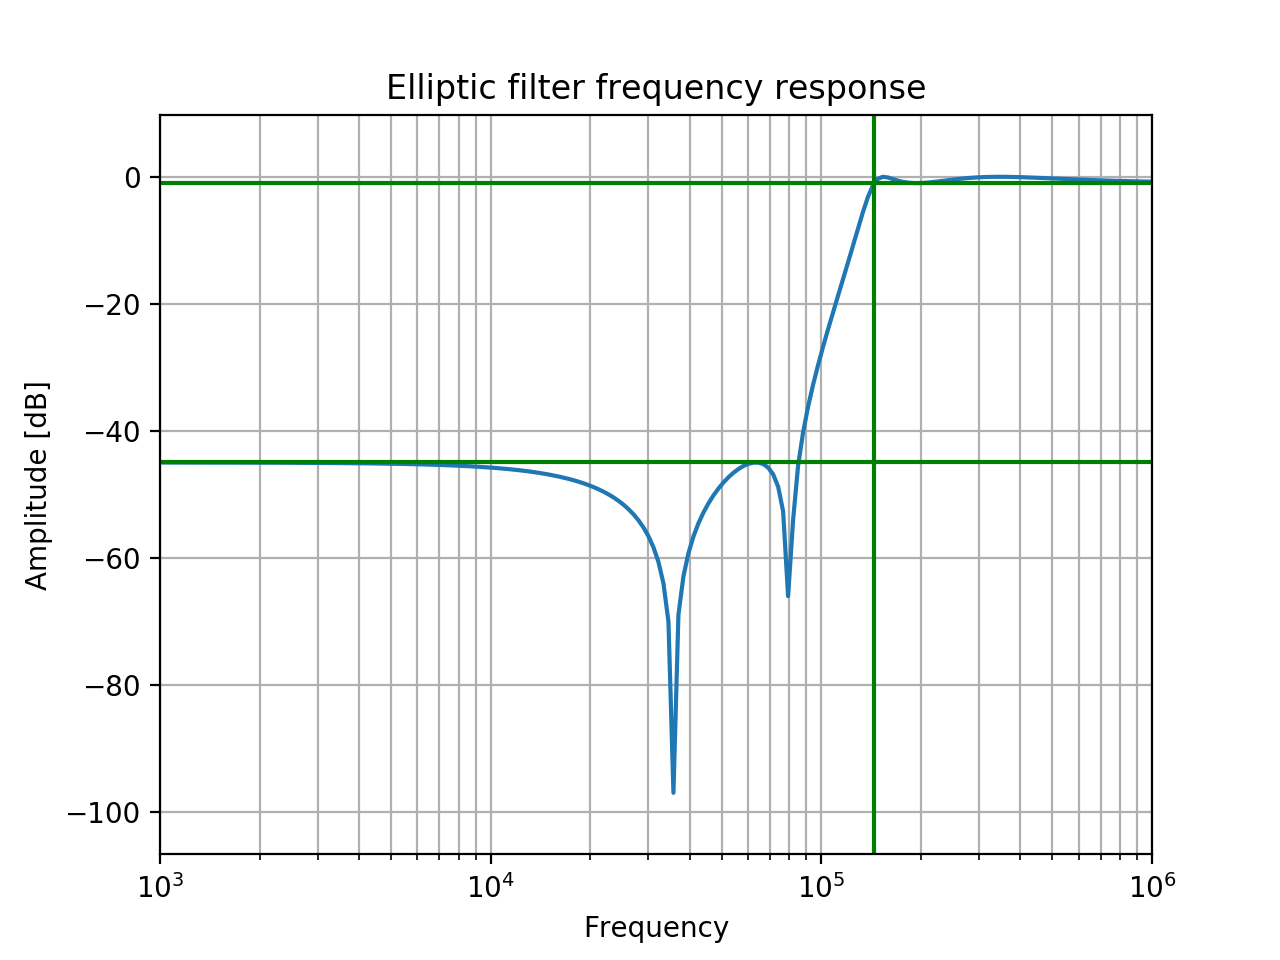
\includegraphics[width=0.6\textwidth]{../Ex3/Resources/cauerbode.png}
\par\end{centering}
\caption{Función transferencia de la aproximación de Cauer para la plantilla propuesta}
\label{bodecauer}
\end{figure}

\begin{figure}[H]
\begin{centering}
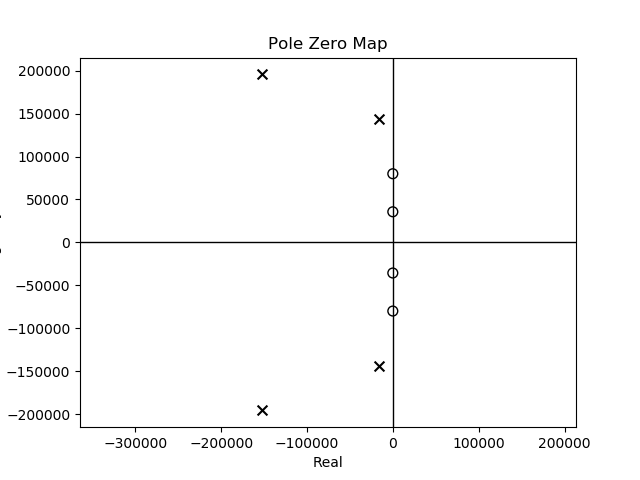
\includegraphics[width=0.5\textwidth]{../Ex3/Resources/poloscauer.png}
\par\end{centering}
\caption{Diagrama de polos y ceros de la aproximación de Cauer para la plantilla propuesta}
\label{poloscauer}
\end{figure}

\subsection{Separación en etapas}
\subsubsection{Funciones transferencia de las etapas}
Para implementar el circuito, al ser de orden 4 la aproximación, se divide esta transferencia en dos funciones bicuadráticas. Estas corresponderán a las transferencias de cada una de las etapas a conectar en cascada, que se implementarán mediante circuitos como el descripto en la sección \ref{marcoteorico}, que llamaremos celdas Sedra.
Las funciones transferencia resultantes son:
\[
H_{1}(s)=\frac{891.25\cdot10^{-3}s^{2}+1.13\cdot10^{9}}{s^{2}+304,3\cdot10^{3}s+6,14\cdot10^{10}}
\]

\[
H_{2}(s)=\frac{s^{2}+6.394\cdot10^{9}}{s^{2}+32.8\cdot10^{3}s+20.96\cdot10^{9}}
\]

Los diagramas de Bode y de polos y ceros para la etapa 1 y 2 se pueden ver en la figuras \ref{bodeetapas} y \ref{polosetapas}, respectivamente.

\begin{figure}[H]
\begin{centering}
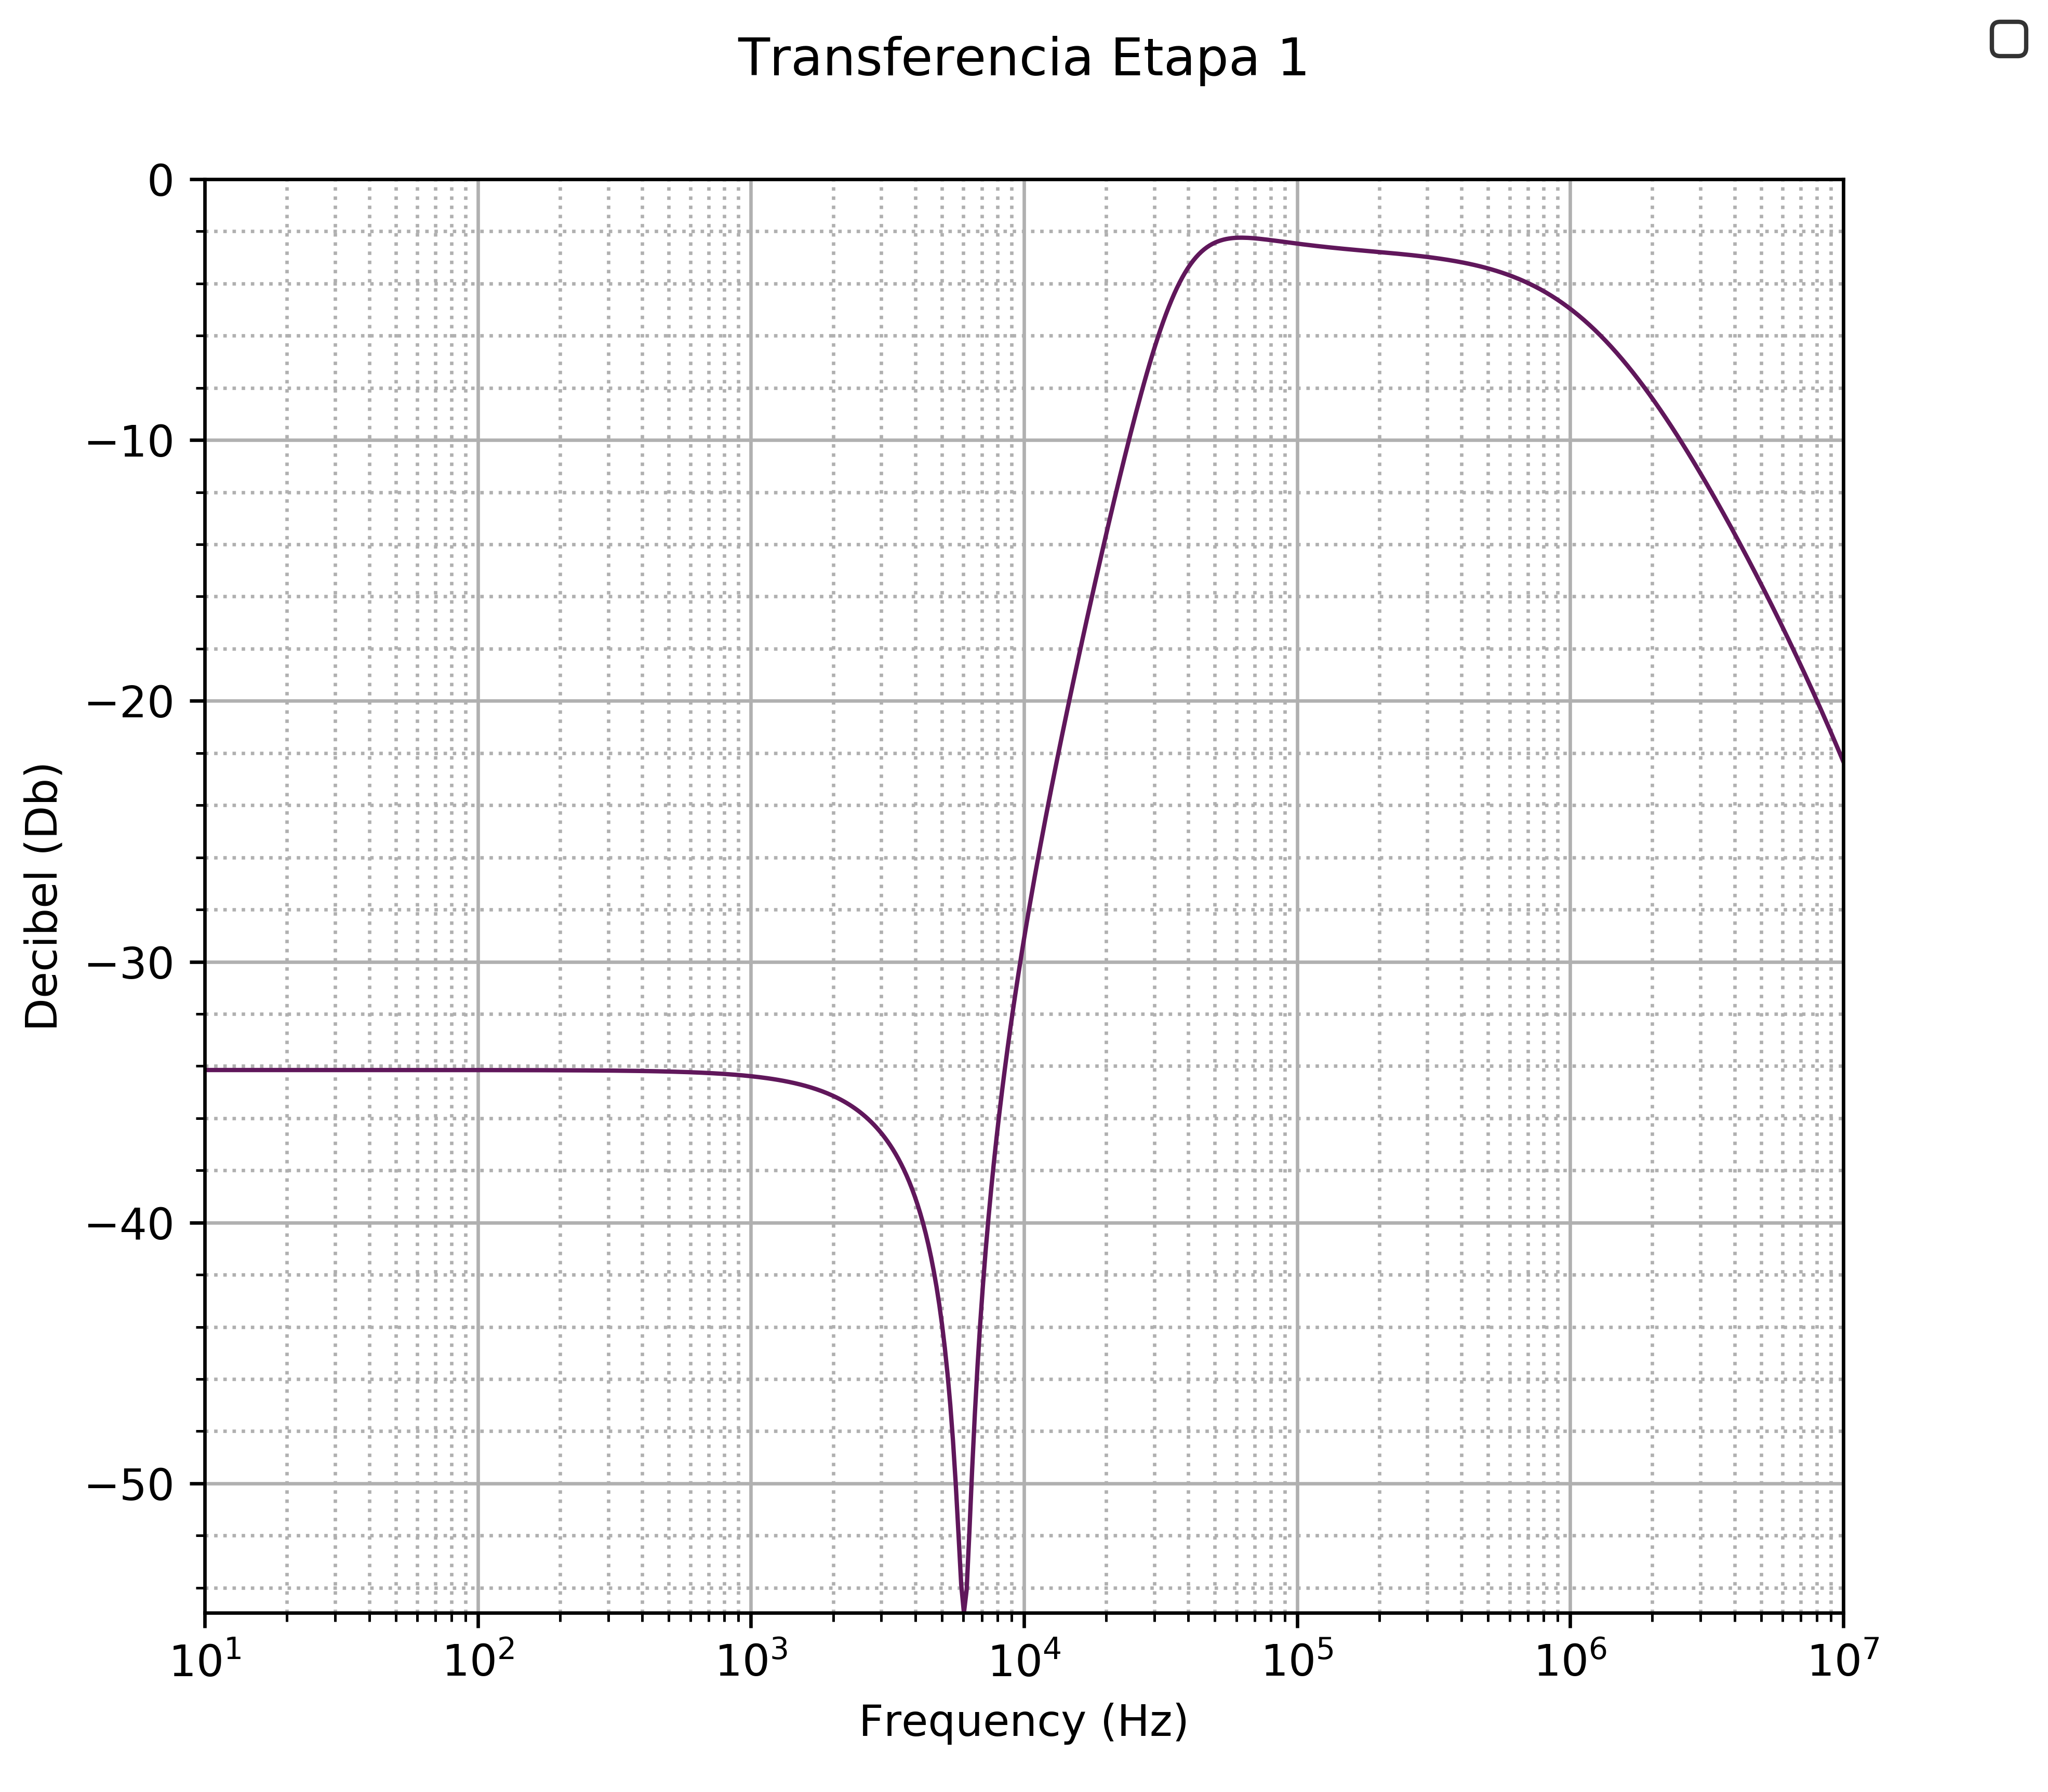
\includegraphics[width=0.45\textwidth]{../Ex3/Resources/bodeetapa1.png}
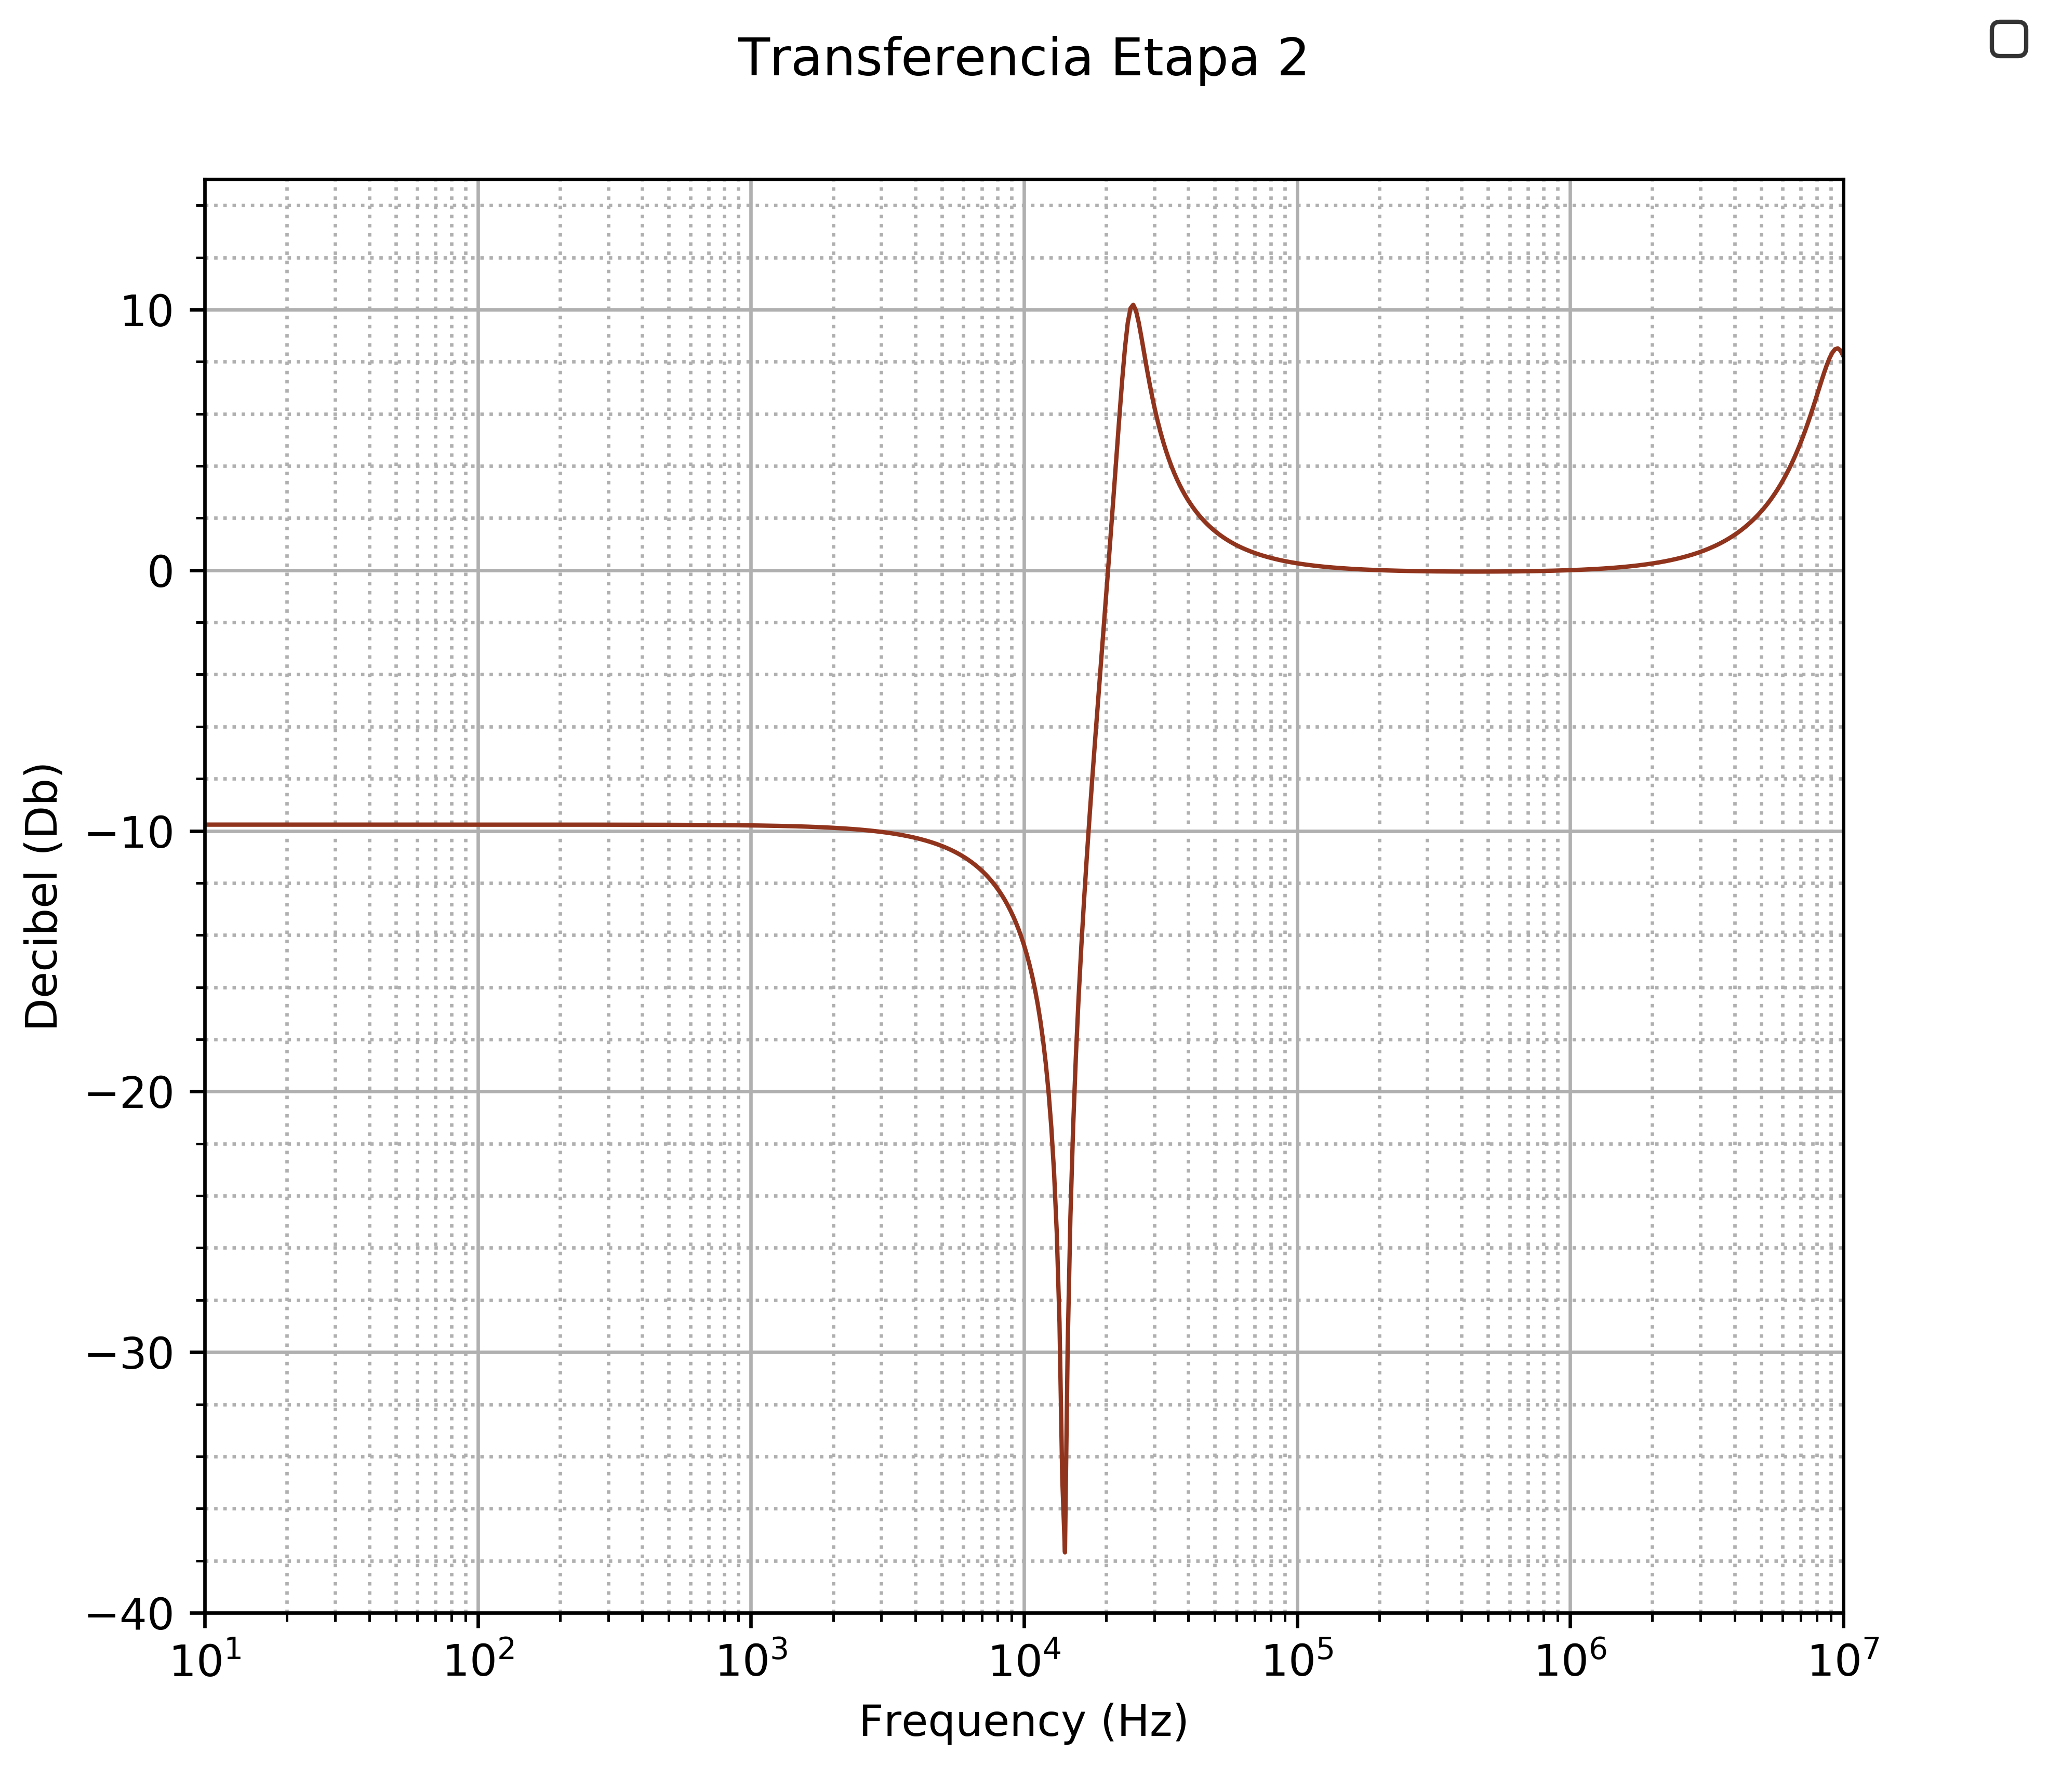
\includegraphics[width=0.45\textwidth]{../Ex3/Resources/bodeetapa2.png}
\par\end{centering}
\caption{Funciones transferencia}
\label{bodeetapas}
\end{figure}

\begin{figure}[H]
\begin{centering}
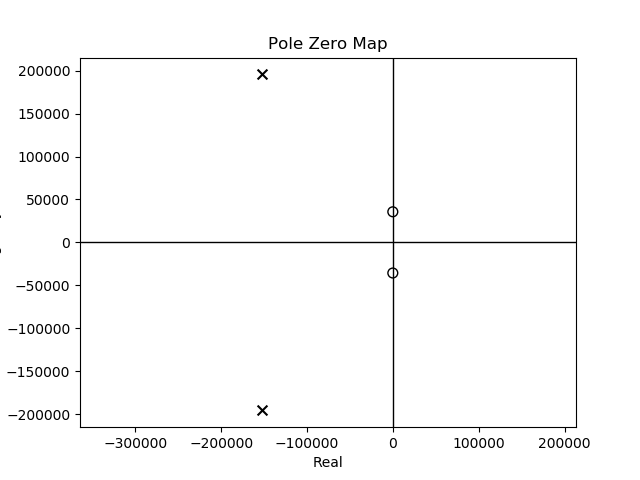
\includegraphics[width=0.45\textwidth]{../Ex3/Resources/polosetapa1.png}
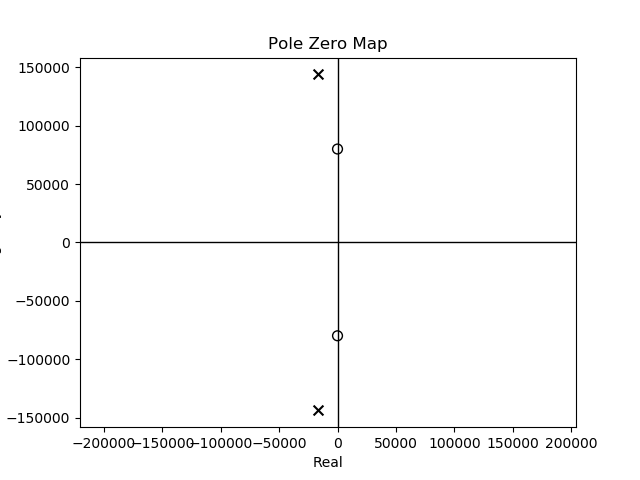
\includegraphics[width=0.45\textwidth]{../Ex3/Resources/polosetapa2.png}
\par\end{centering}
\caption{Diagramas de polos y ceros (etapa 1 izquierda, etapa 2 derecha)}
\label{polosetapas}
\end{figure}



\subsubsection{Asociación de polos y ceros para cada etapa}
Las funciones transferencia para cada etapa fueron obtenidas con asistencia de funciones de la librería \emph{SciPy} de Python, que selecciona de forma conveniente los polos y los ceros de cada una. Para obtener dos transferencias lo más planas posible, se asocian los polos y ceros interiores y exteriores. % revisar

\subsection{Implementación de etapas: celdas Sedra} 
Cada una de las etapas se implementó con un circuito (Figura \ref{sedracircs}) HPB idéntico a los descriptos por los autores de la publicación mencionada en la sección \ref{marcoteorico}. A continuación, se detalla el procedimiento de diseño.
\subsubsection{Valores reales del circuito}\label{valoresetapassedra}
A partir de las funciones transferencia obtenidas, se obtienen para las etapas 1 y 2 los valores del Cuadro \ref{tablavalorestransferencia}. Se añaden al mismo los valores comerciales disponibles para la implementación práctica del filtro en un circuito.

\begin{table}[H]
\begin{centering}
\begin{tabular}{|c|c|c|}
\hline 
Parámetro & Etapa 1 & Etapa 2\tabularnewline
\hline 
\hline 
$\omega_{0}$ & 280332 rad/s & 156890 rad/s\tabularnewline
\hline 
Q & 0.986 & 6.42\tabularnewline
\hline 
$n_{2}$ & $794.3\cdot10^{-3}$ & 1\tabularnewline
\hline 
\end{tabular}
\par\end{centering}
\caption{Valores tomados de la transferencia de cada etapa}
\label{tablavalorestransferencia}
\end{table}

Se calculan con estos valores los parámetros de diseño y los componentes del circuito HPB. Se elige $C=5nF$ y $G_{b}=1k\Omega$ y se calculan los demás componentes del circuito:

\begin{figure}[H]
\begin{centering}
\begin{tabular}{|c|c|c|c|}
\hline 
Parámetro & Fórmula & Etapa 1 & Etapa 2\tabularnewline
\hline 
\hline 
K & $1+\frac{(1-\frac{Q_{0}}{Q})}{2*Q_{0}^{2}}$ & 0.904 & 1.011\tabularnewline
\hline 
k & $n_{2}*\frac{(\frac{\omega_{z}}{\omega_{0}})^{2}}{1-\frac{Q_{0}}{Q}}$& 0.0308 & -0.706\tabularnewline
\hline 
n & $k*(1-\frac{Q_{0}}{K*Q})$& & \tabularnewline
\hline 
m & $k*(K-1)*\frac{(1+2*Q_{0}^{2}*(\frac{\omega_{0}}{\omega_{z}})^{2})}{K}$ & -3,56 & -0.623\tabularnewline
\hline 
\end{tabular}
\par\end{centering}
\caption{Parámetros intrínsecos de cada celda}
\end{figure}

\begin{figure}[H]
\begin{centering}
\begin{tabular}{|c|c|c|c|c|c|}

\hline 
Componente & Relación & Etapa 1 & Etapa 2 & Etapa 1 & Etapa 2\tabularnewline
\hline 

\multicolumn{2}{|c|}{} & \multicolumn{2}{|c|}{Valores calculados} & \multicolumn{2}{|c|}{Valores comerciales} \tabularnewline
\hline
\hline 
C$_{3}$ & (K-1){*}G$_{b}$ & 5nF & 5nF & 4.7nF & 4.7nF\tabularnewline
\hline 
G$_{a1}$ & (1-k){*}G$_{a}$ & $\frac{1}{67.9\Omega}$ & $\frac{1}{11928.26\Omega}$ & $\frac{1}{68\Omega}$ & $\frac{1}{12000\Omega}$\tabularnewline
\hline 
G$_{a2}$ & k{*}G$_{a}$& $\frac{1}{2877.97\Omega}$ & $\frac{1}{14146\Omega}$ & $\frac{1}{3000\Omega}$ & $\frac{1}{15000\Omega}$\tabularnewline
\hline 
$G_{41}$ & $(1-n){*}G_{4}$& $\frac{1}{269\Omega}$ & $\frac{1}{6014.13\Omega}$ & $\frac{1}{270\Omega}$ & $\frac{1}{6200\Omega}$\tabularnewline
\hline 
$G_{42}$ & $n{*}G_{4}$& $\frac{1}{11547.46\Omega}$ & $\frac{1}{12486.56\Omega}$ & $\frac{1}{12000\Omega}$ & $\frac{1}{12000\Omega}$\tabularnewline
\hline 
$C_{21}$ & $(1-m){*}C$ & 4.61nF & 0.363nF & 4.7nF & 0.39nF\tabularnewline
\hline 
$C_{22}$ & $m*C$ & 0.385nF & 4.63nF & 0.39nF & 4.7nF\tabularnewline
\hline 
\end{tabular}
\par\end{centering}
\caption{Selección de componentes para las etapas}
\end{figure}


\subsubsection{Selección del orden de las etapas: rango dinámico}
Para conservar el máximo rango dinámico posible, se ordenan las etapas a conectar en cascada según sus valores de Q de forma creciente. % completar


\subsubsection{Asociación de impedancias para conexión en cascada}
Para conservar las funciones transferencia de cada etapa y hacer que la transferencia total del circuito sea el producto de las mismas, debe evitarse que las etapas se carguen entre sí. A tal efecto, la impedancia de salida de cada etapa debe ser mucho menor que la impedancia de entrada de la etapa que le sigue. La impedancia de salida de la etapa 1 y la impedancia de entrada de la etapa 2 se pueden ver graficadas en frecuencia en la Figura \ref{imptodo}.

\begin{figure}[H]
    \centering
    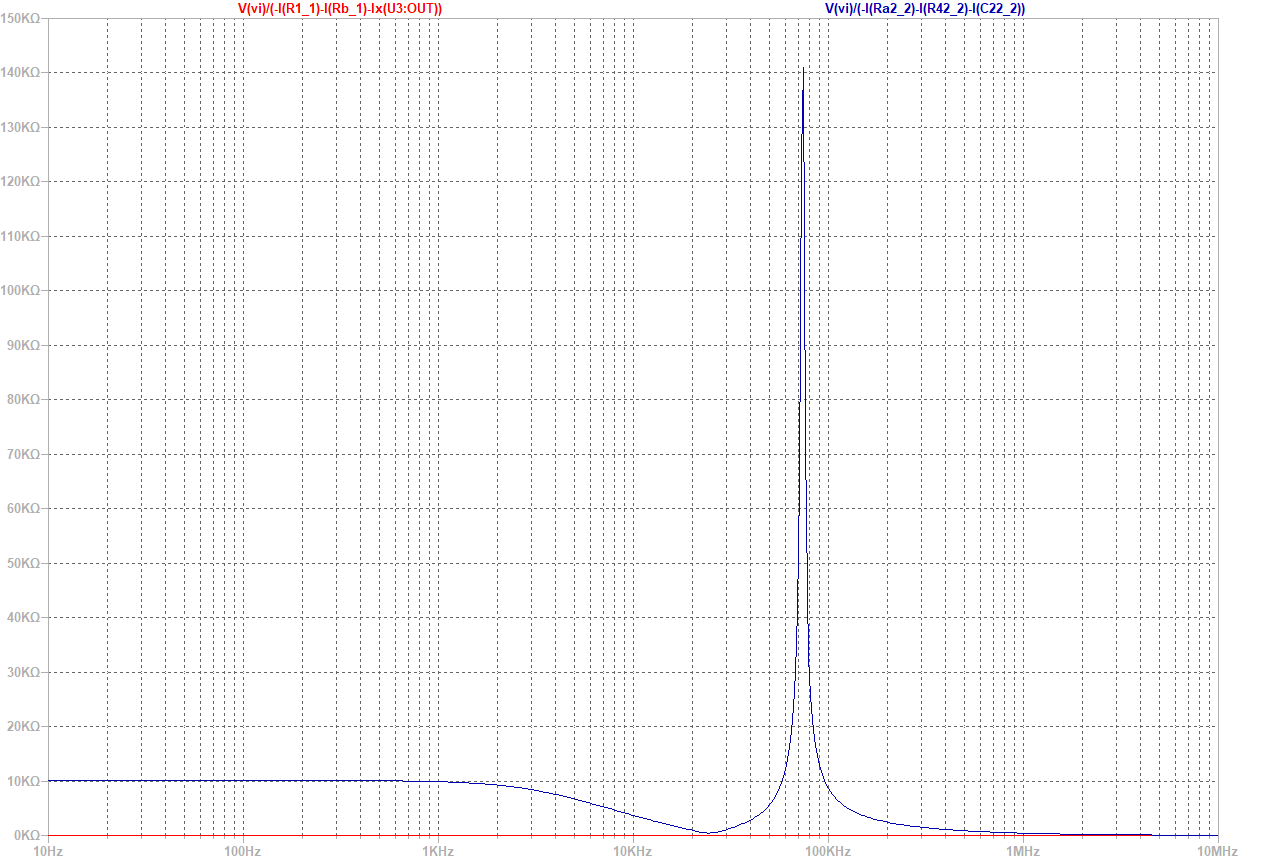
\includegraphics[width=0.6\textwidth]{../Ex3/Resources/imptodo.png}
    \caption{Impedancia de salida de la etapa 1 (rojo) y de entrada de la etapa 2 (azul)}
    \label{imptodo}
\end{figure}

Se puede observar que estas impedancias no son comparables, por lo que se considera despreciable la carga entre las etapas. Aún en la zona en la que se acercan más, como se puede observar en el detalle de la Figura \ref{impdetalle}, la impedancia de entrada de la etapa 2 es 150 veces más grande que la impedancia de salida de la etapa 1.

\begin{figure}[H]
    \centering
    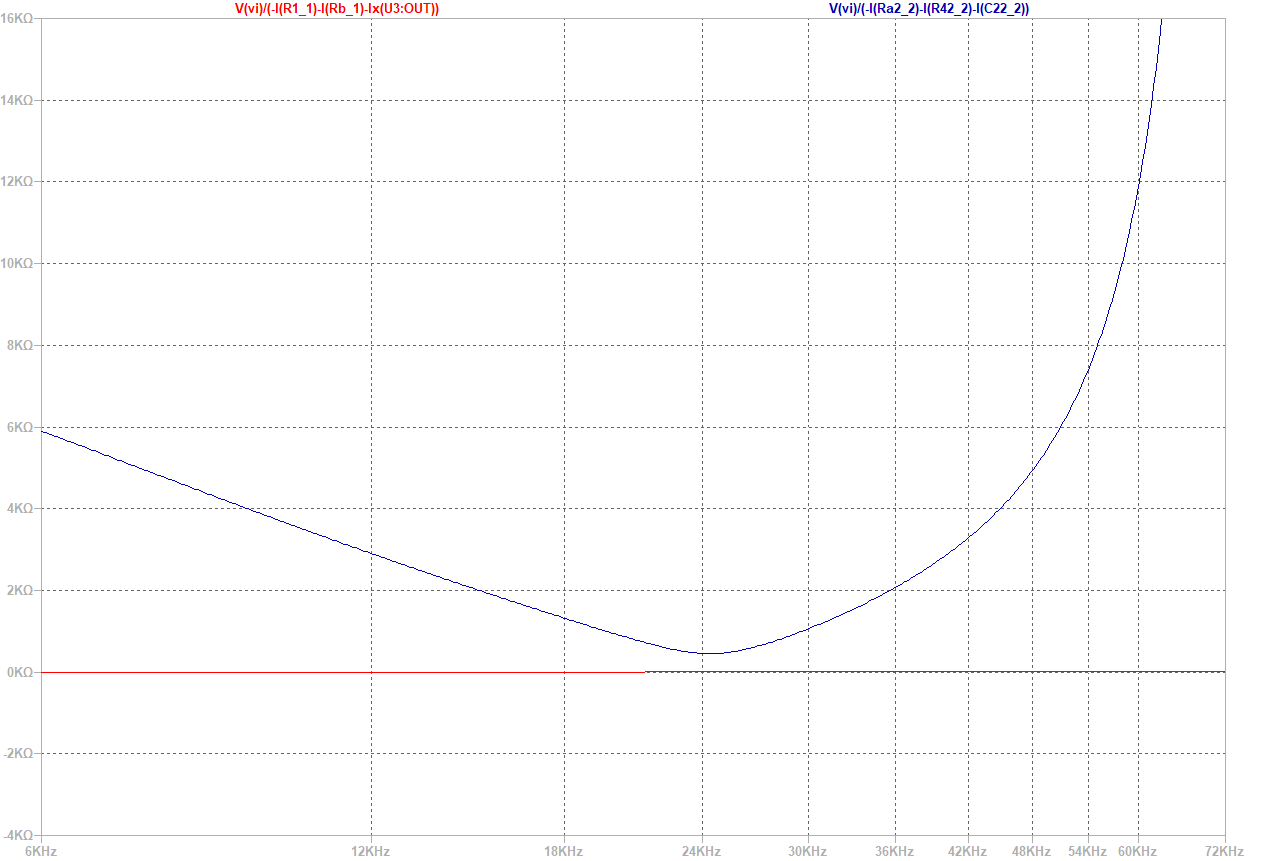
\includegraphics[width=0.6\textwidth]{../Ex3/Resources/impdetalle.png}
    \caption{Detalle de la comparación de impedancias}
    \label{impdetalle}
\end{figure}

\subsection{Parámetros del circuito completo}
A continuación, se detallan parámetros relevantes del circuito completo.
\subsubsection{Impedancia de entrada}
La impedancia de entrada del circuito es la misma que la de la primera etapa. Esta se puede observar en la Figura \ref{impentetapa1}. Se puede ver que es menor al valor mínimo de $30k\Omega$ propuesto en la plantilla, por lo que se optó por anteponer un circuito \emph{buffer} en la entrada para aumentarla a ordenes de gigaohmios.

\begin{figure}[H]
    \centering
    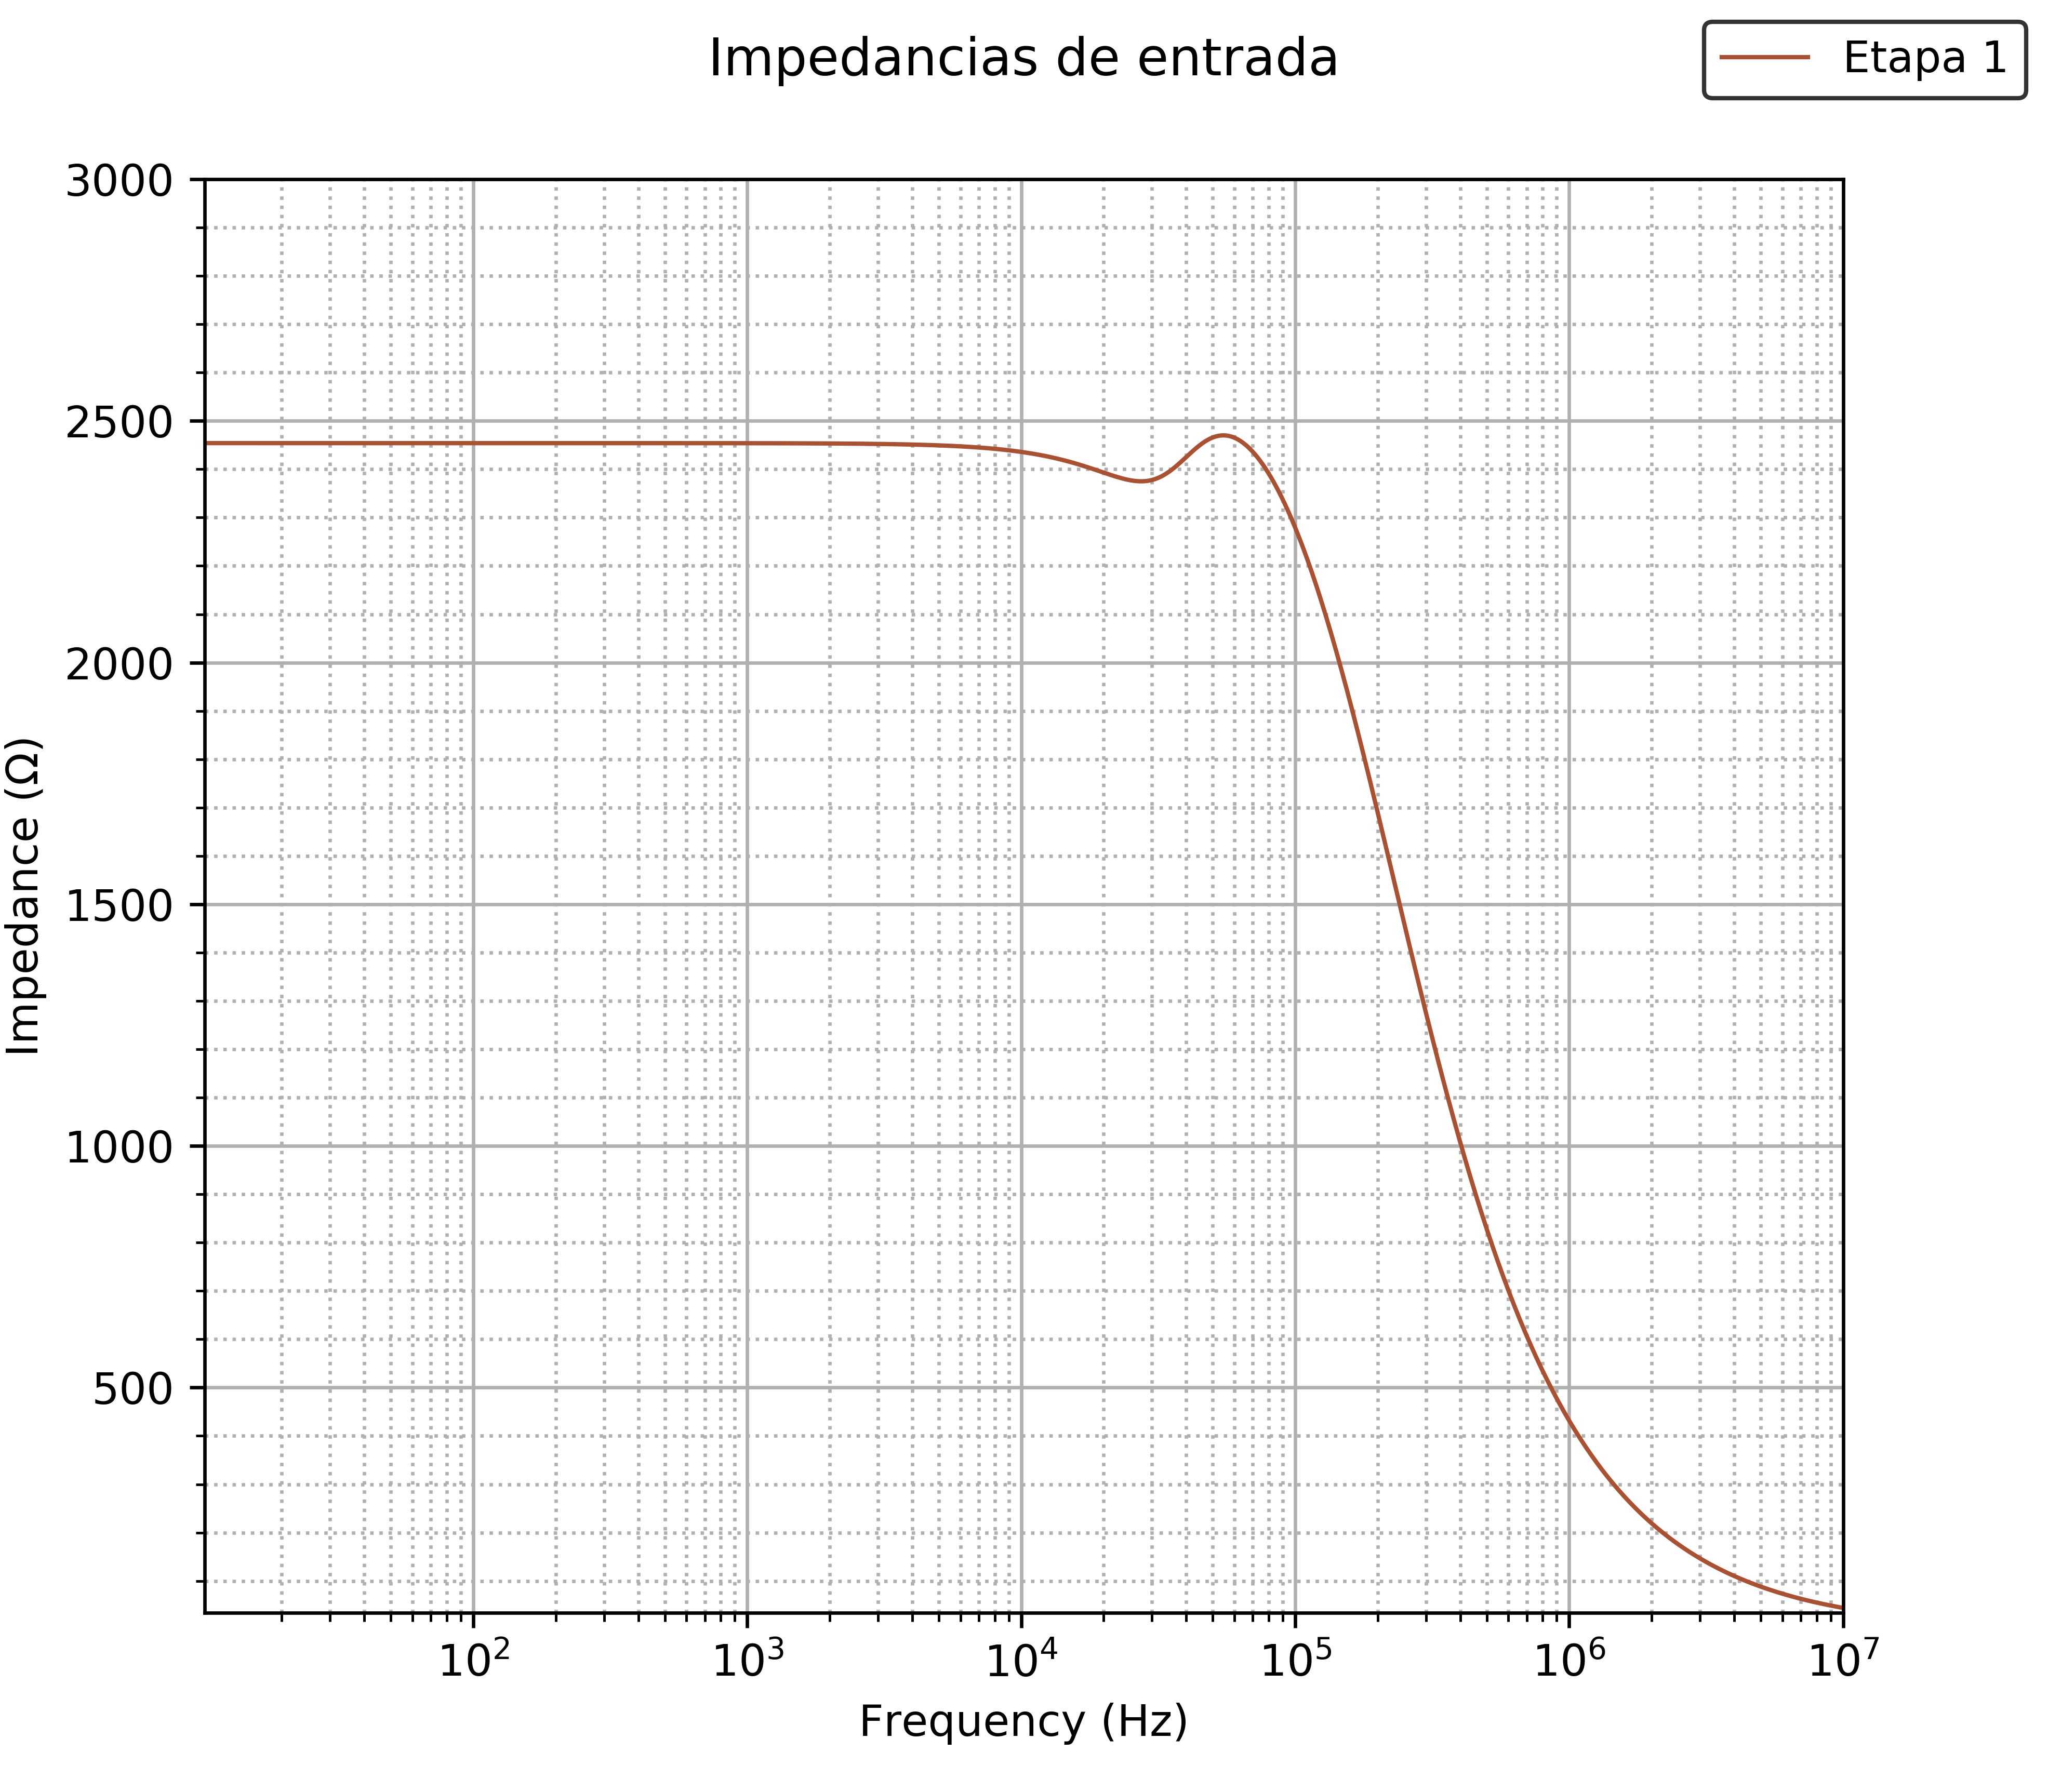
\includegraphics[width=0.6\textwidth]{../Ex3/Resources/impentetapa1.png}
    \caption{Impedancia de entrada del circuito total}
    \label{impentetapa1}
\end{figure}

\subsubsection{Impedancia de salida}
La impedancia de salida del circuito total, como se puede observar en la Figura \ref{impsaltotal}, resultó satisfactoriamente baja para todo el rango de frecuencias en consideración.

\begin{figure}[H]
    \centering
    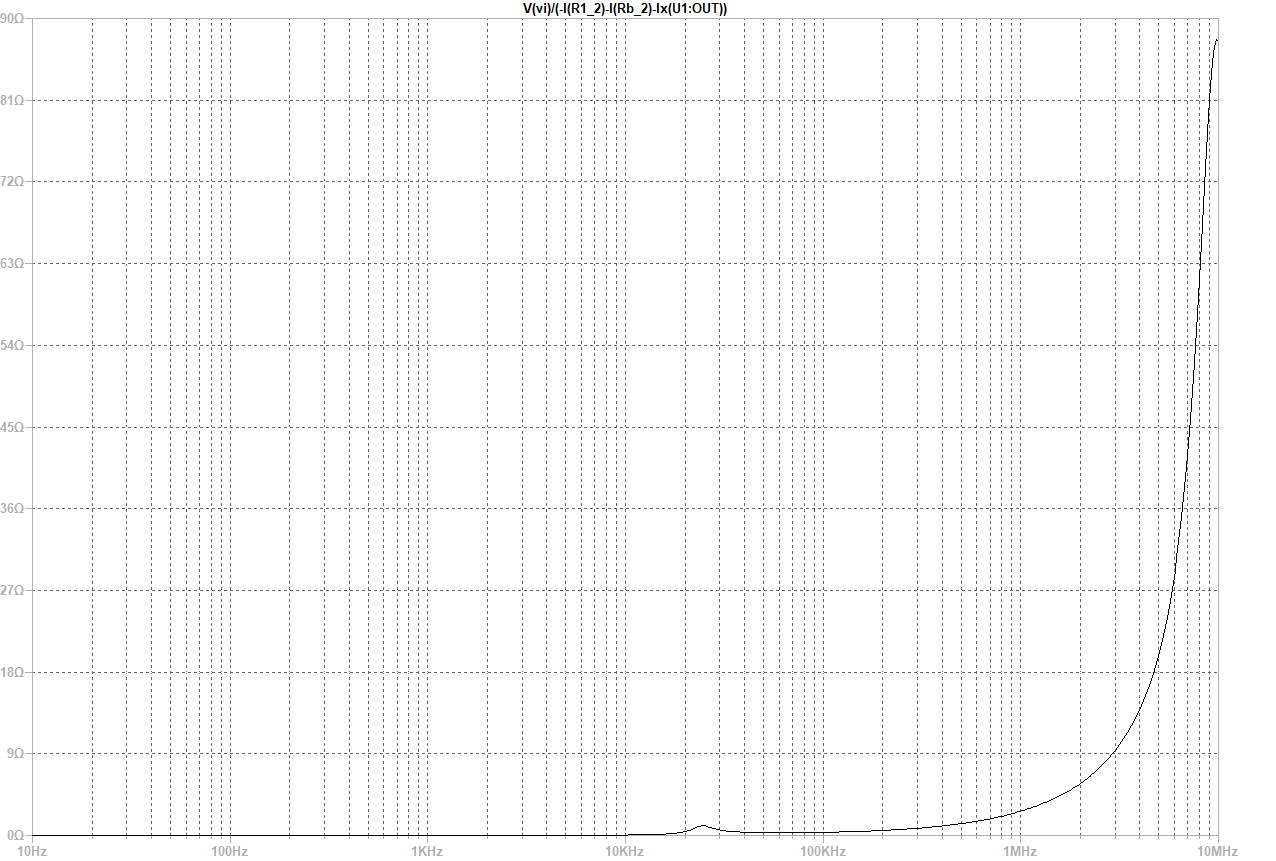
\includegraphics[width=0.6\textwidth]{../Ex3/Resources/impsaltotal.png}
    \caption{Impedancia de salida del circuito total}
    \label{impsaltotal}
\end{figure}

\subsubsection{Transferencia total del circuito} \label{transftotalcirc}
Como se detalló en la sección \ref{valoresetapassedra}, se utilizaron valores comerciales cercanos a los teóricos para todos los componentes del circuito. Naturalmente, se simularon ambas instancias del circuito (con valores reales y comerciales), y se comprobó que la transferencia obtenida no dejara de cumplir con los parámetros especificados. Estas mediciones se pueden ver en la Figura \ref{exactosvscomerciales}.
\begin{figure}[H]
    \centering
    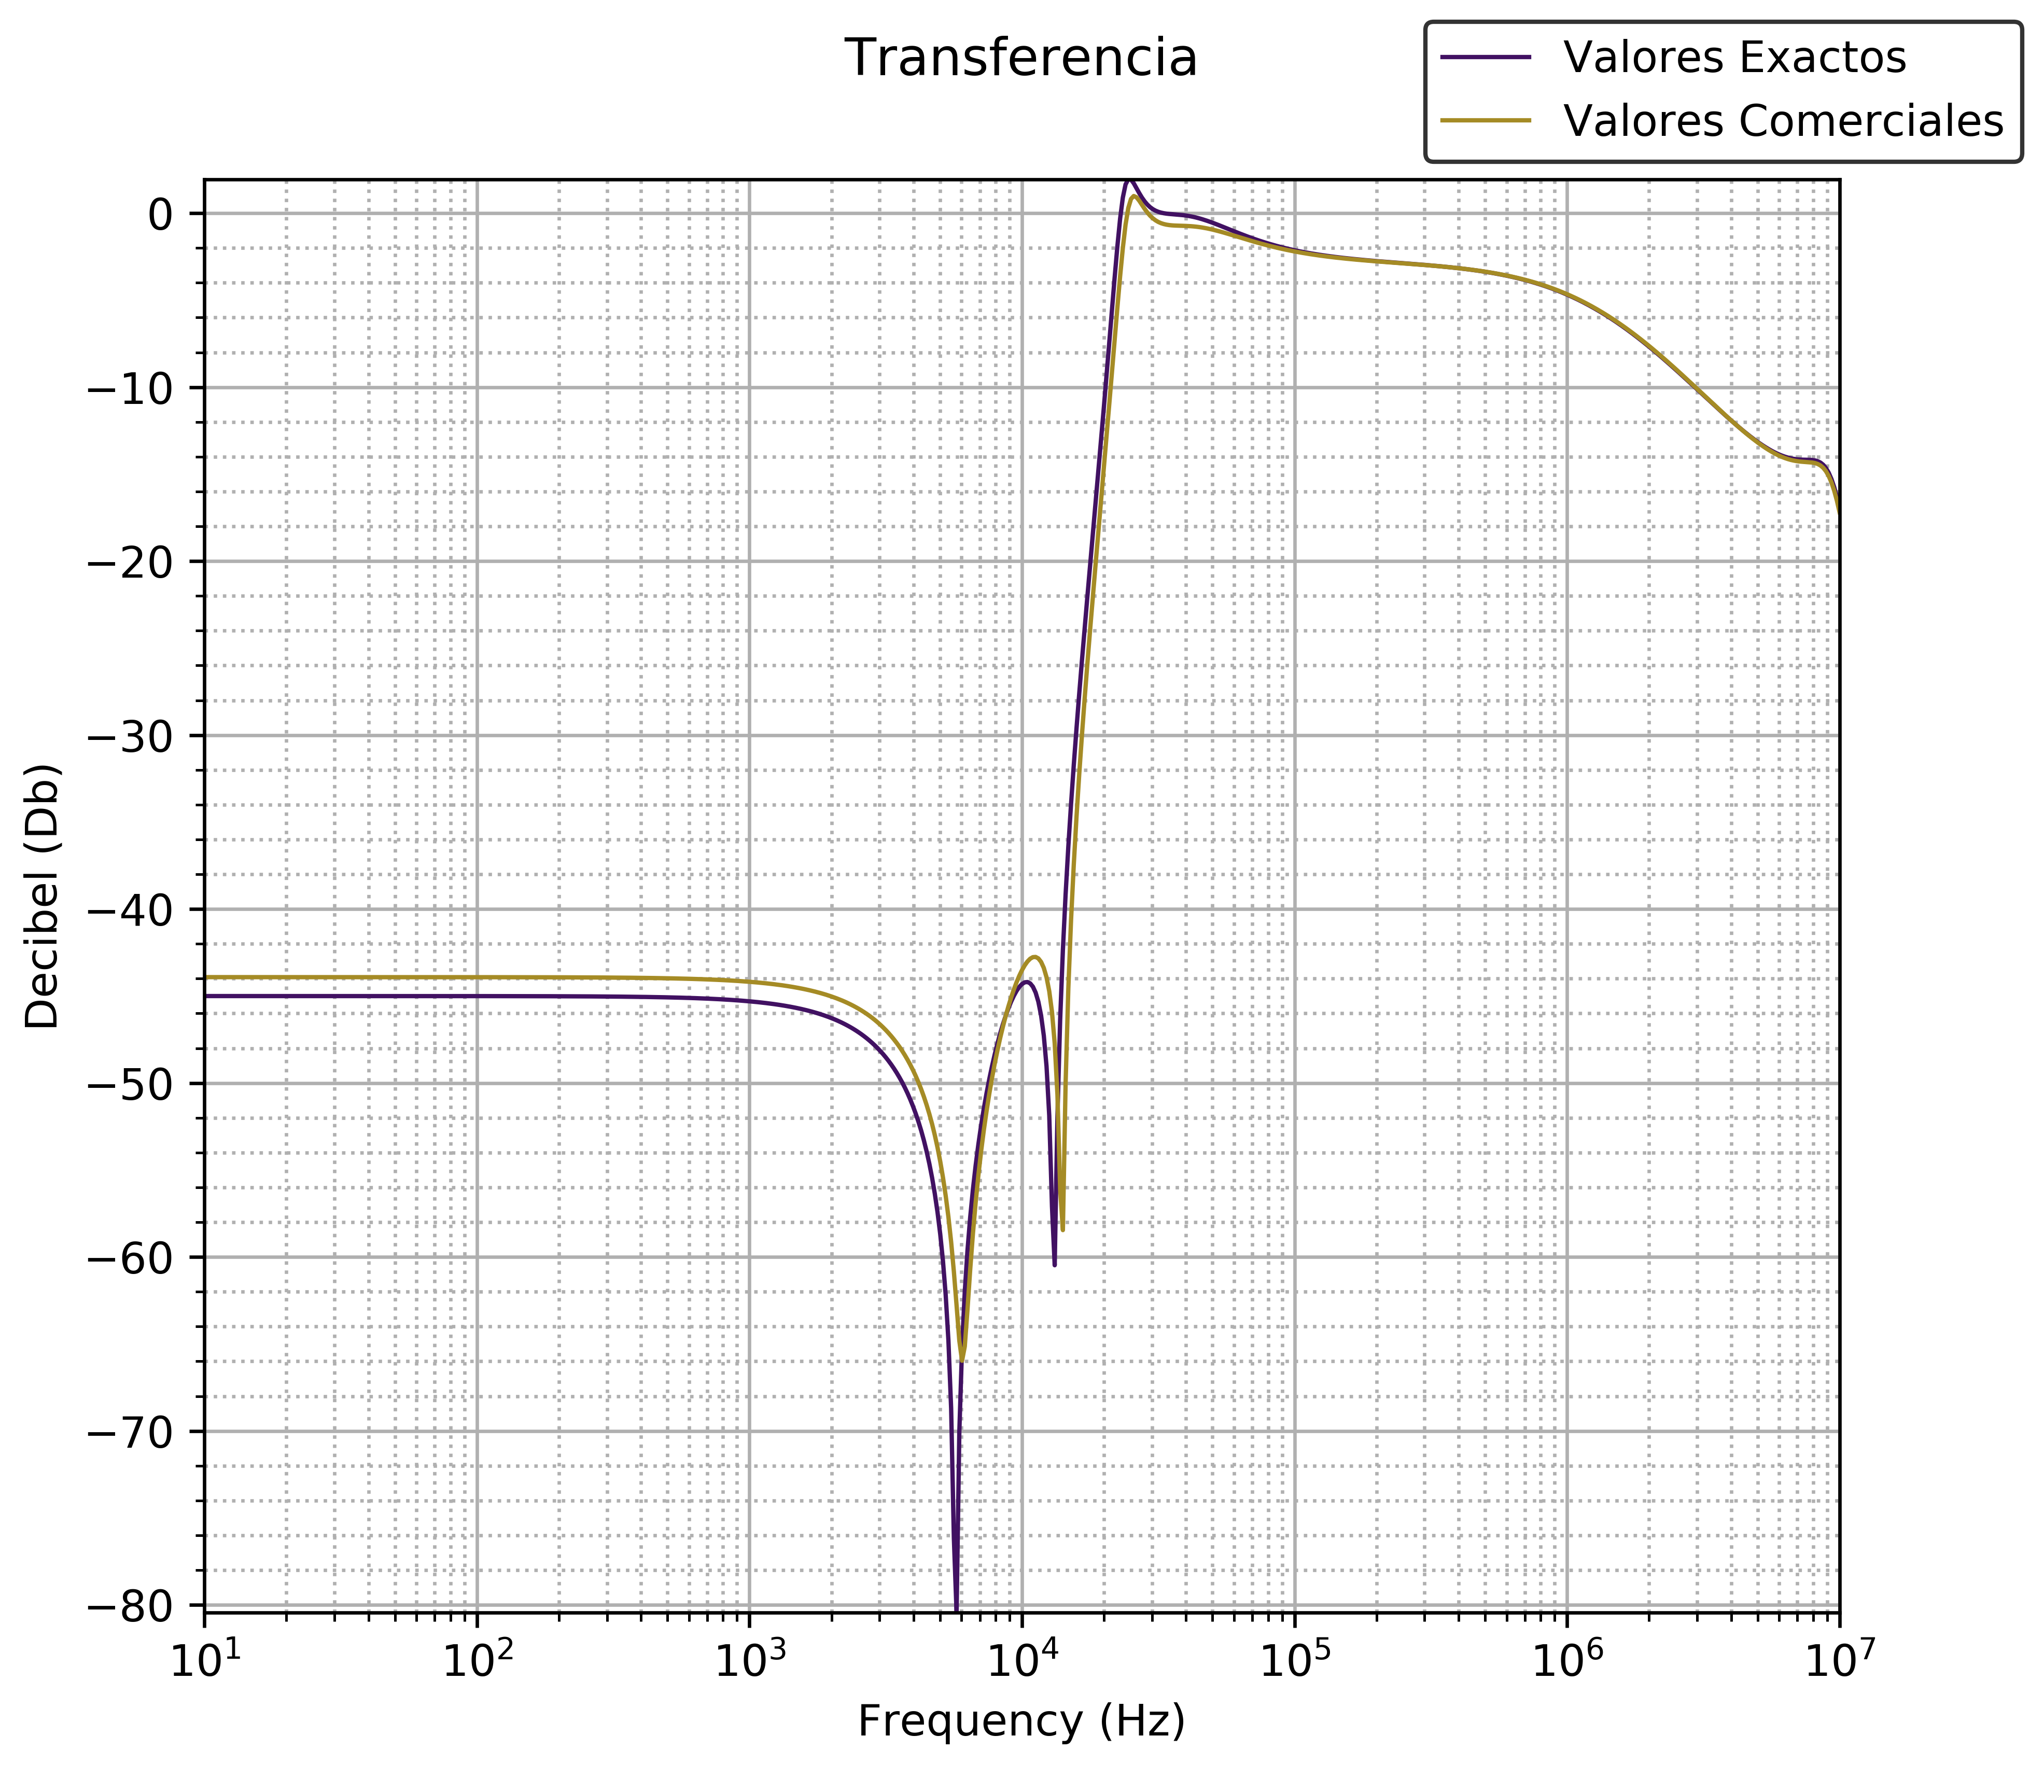
\includegraphics[width=0.6\textwidth]{../Ex3/Resources/exactosvscomerciales.png}
    \caption{Transferencia del circuito: comparación con valores teóricos}
    \label{exactosvscomerciales}
\end{figure}

Asimismo, se consideraron los efectos de las tolerancias de dichos componentes en el desempeño del filtro: se tomaron variaciones del 10\% para capacitores, y del 1\% para resistencias, ya que todas ellas son de montaje superficial. La simulación de Montecarlo del circuito para dichas tolerancias se observa en la Figura \ref{transfmontecarlo}. Se puede notar que a pesar del error en los valores, el circuito no deja de cumplir con lo requerido en la banda atenuada. Para los peores casos, en la banda pasante se observa algo de atenuación indeseada, de órdenes pequeños. Los resultados se consideraron satisfactorios a pesar de esto último.

\begin{figure}[H]
    \centering
    \includegraphics[width=0.6\textwidth]{../Ex3/Resources/transfmontecarlo.png}
    \caption{Transferencia del circuito: Montecarlo}
    \label{transfmontecarlo}
\end{figure}

En el diagrama de Montecarlo de la fase, observado en la Figura \ref{montecarlofase}, se ve que hay un cambio de fase repentino en frecuencias cercanas a los 5kHz. Esto se debe al cero de la primera etapa, que se encuentra sobre el eje imaginario: en este punto de frecuencias, este cero produce un cambio de fase. Para ciertos valores de tolerancias este cero se encuentra en el semiplano derecho, generando un cambio de fase de -90 grados; para otros, se mantiene en el semiplano izquierdo y genera un cambio de fase de 90 grados. Es preferible que se mantengan en el semiplano izquierdo, ya que de pasar al derecho podrían causar problemas de estabilidad en el sistema.

\begin{figure}[H]
    \centering
    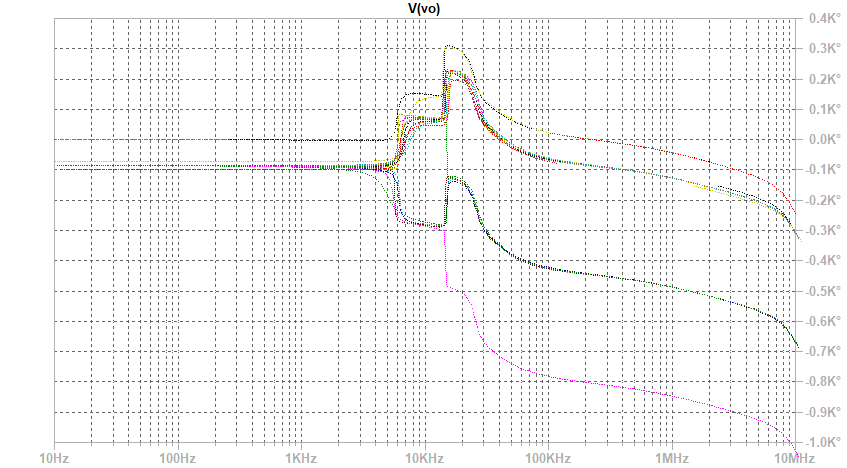
\includegraphics[width=0.6\textwidth]{../Ex3/Resources/montecarlofase.png}
    \caption{Transferencia del circuito: Montecarlo}
    \label{montecarlofase}
\end{figure}

Se realizó como parte del análisis de tolerancias una serie de histogramas para los parámetros $f_{0}$ y $Q$ de cada polo para cada etapa. Estos se observan en las figuras \ref{sedrahistf0} y \ref{sedrahistq}, respectivamente.

\begin{figure}[H]
    \centering
    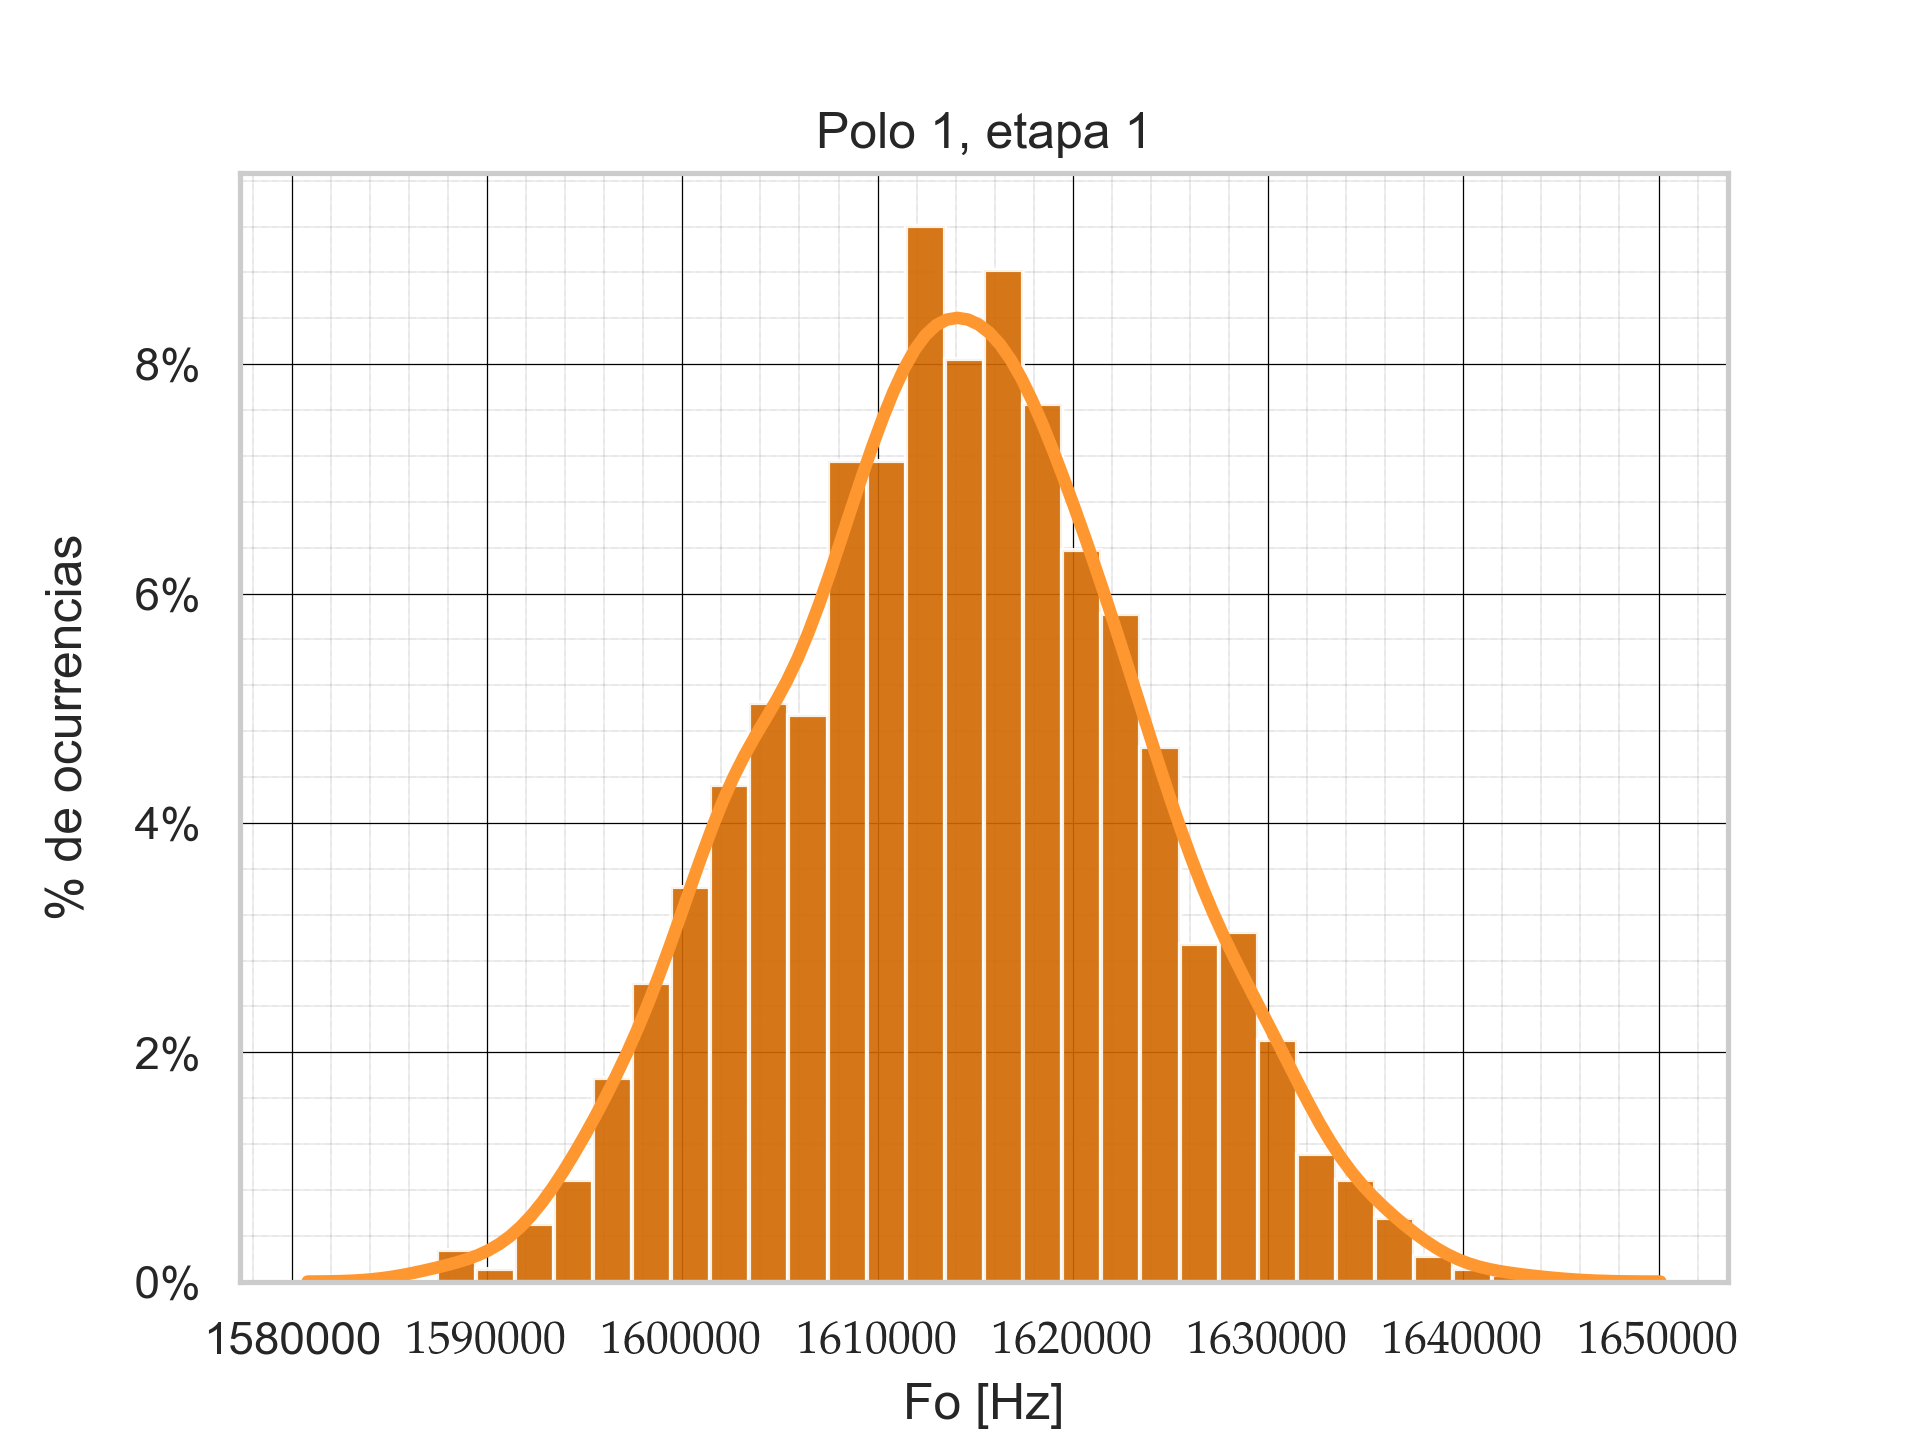
\includegraphics[width=0.45\textwidth]{../Ex3/Resources/histograma_w0_poles_00.png}
    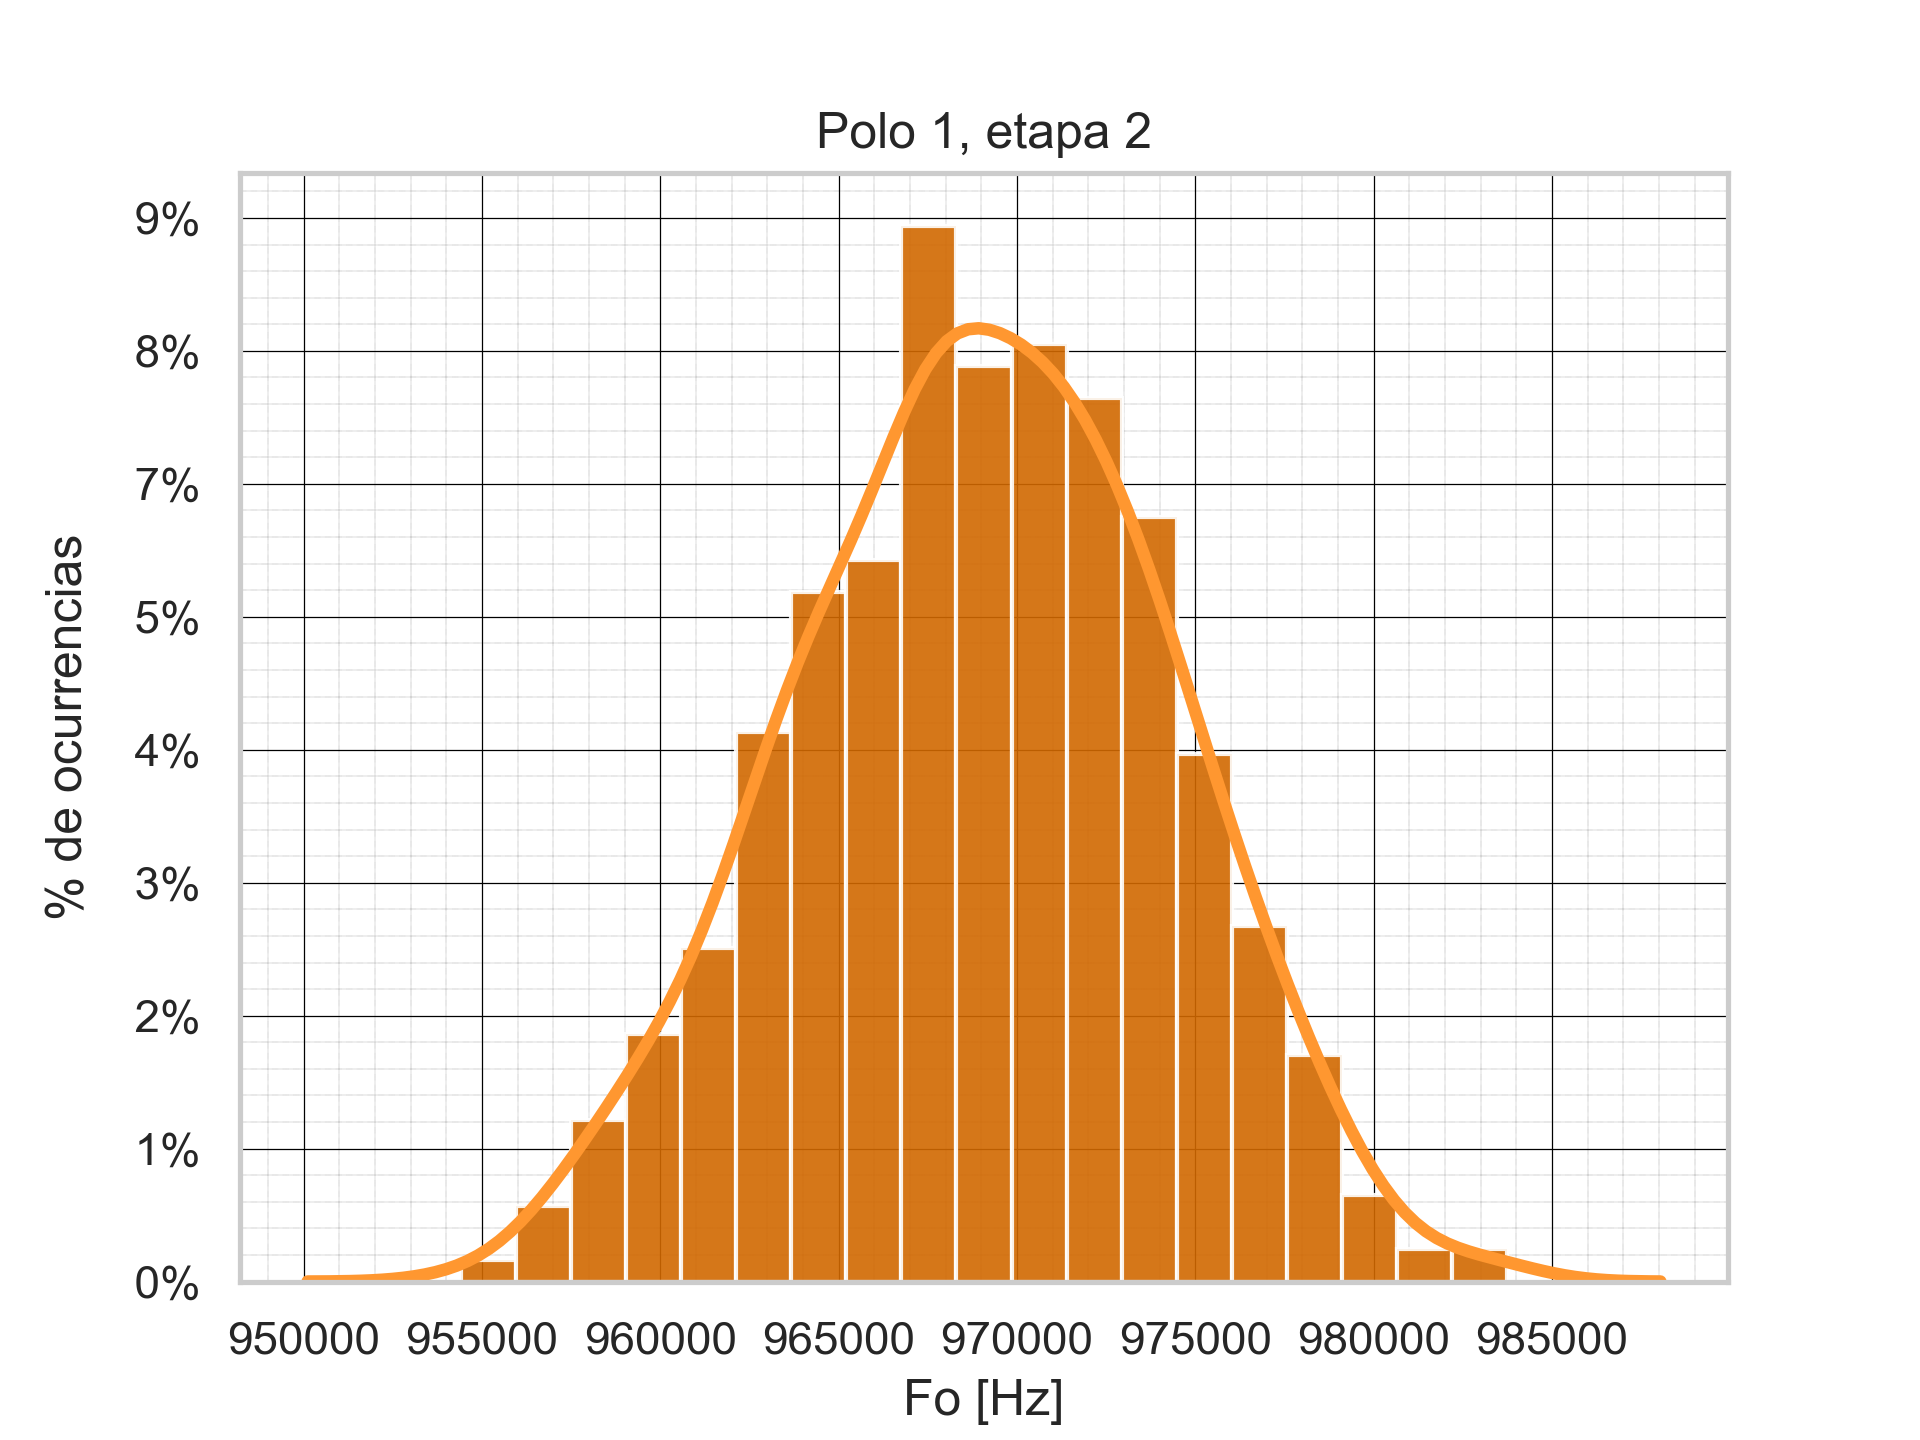
\includegraphics[width=0.45\textwidth]{../Ex3/Resources/histograma_w0_poles_01.png}
    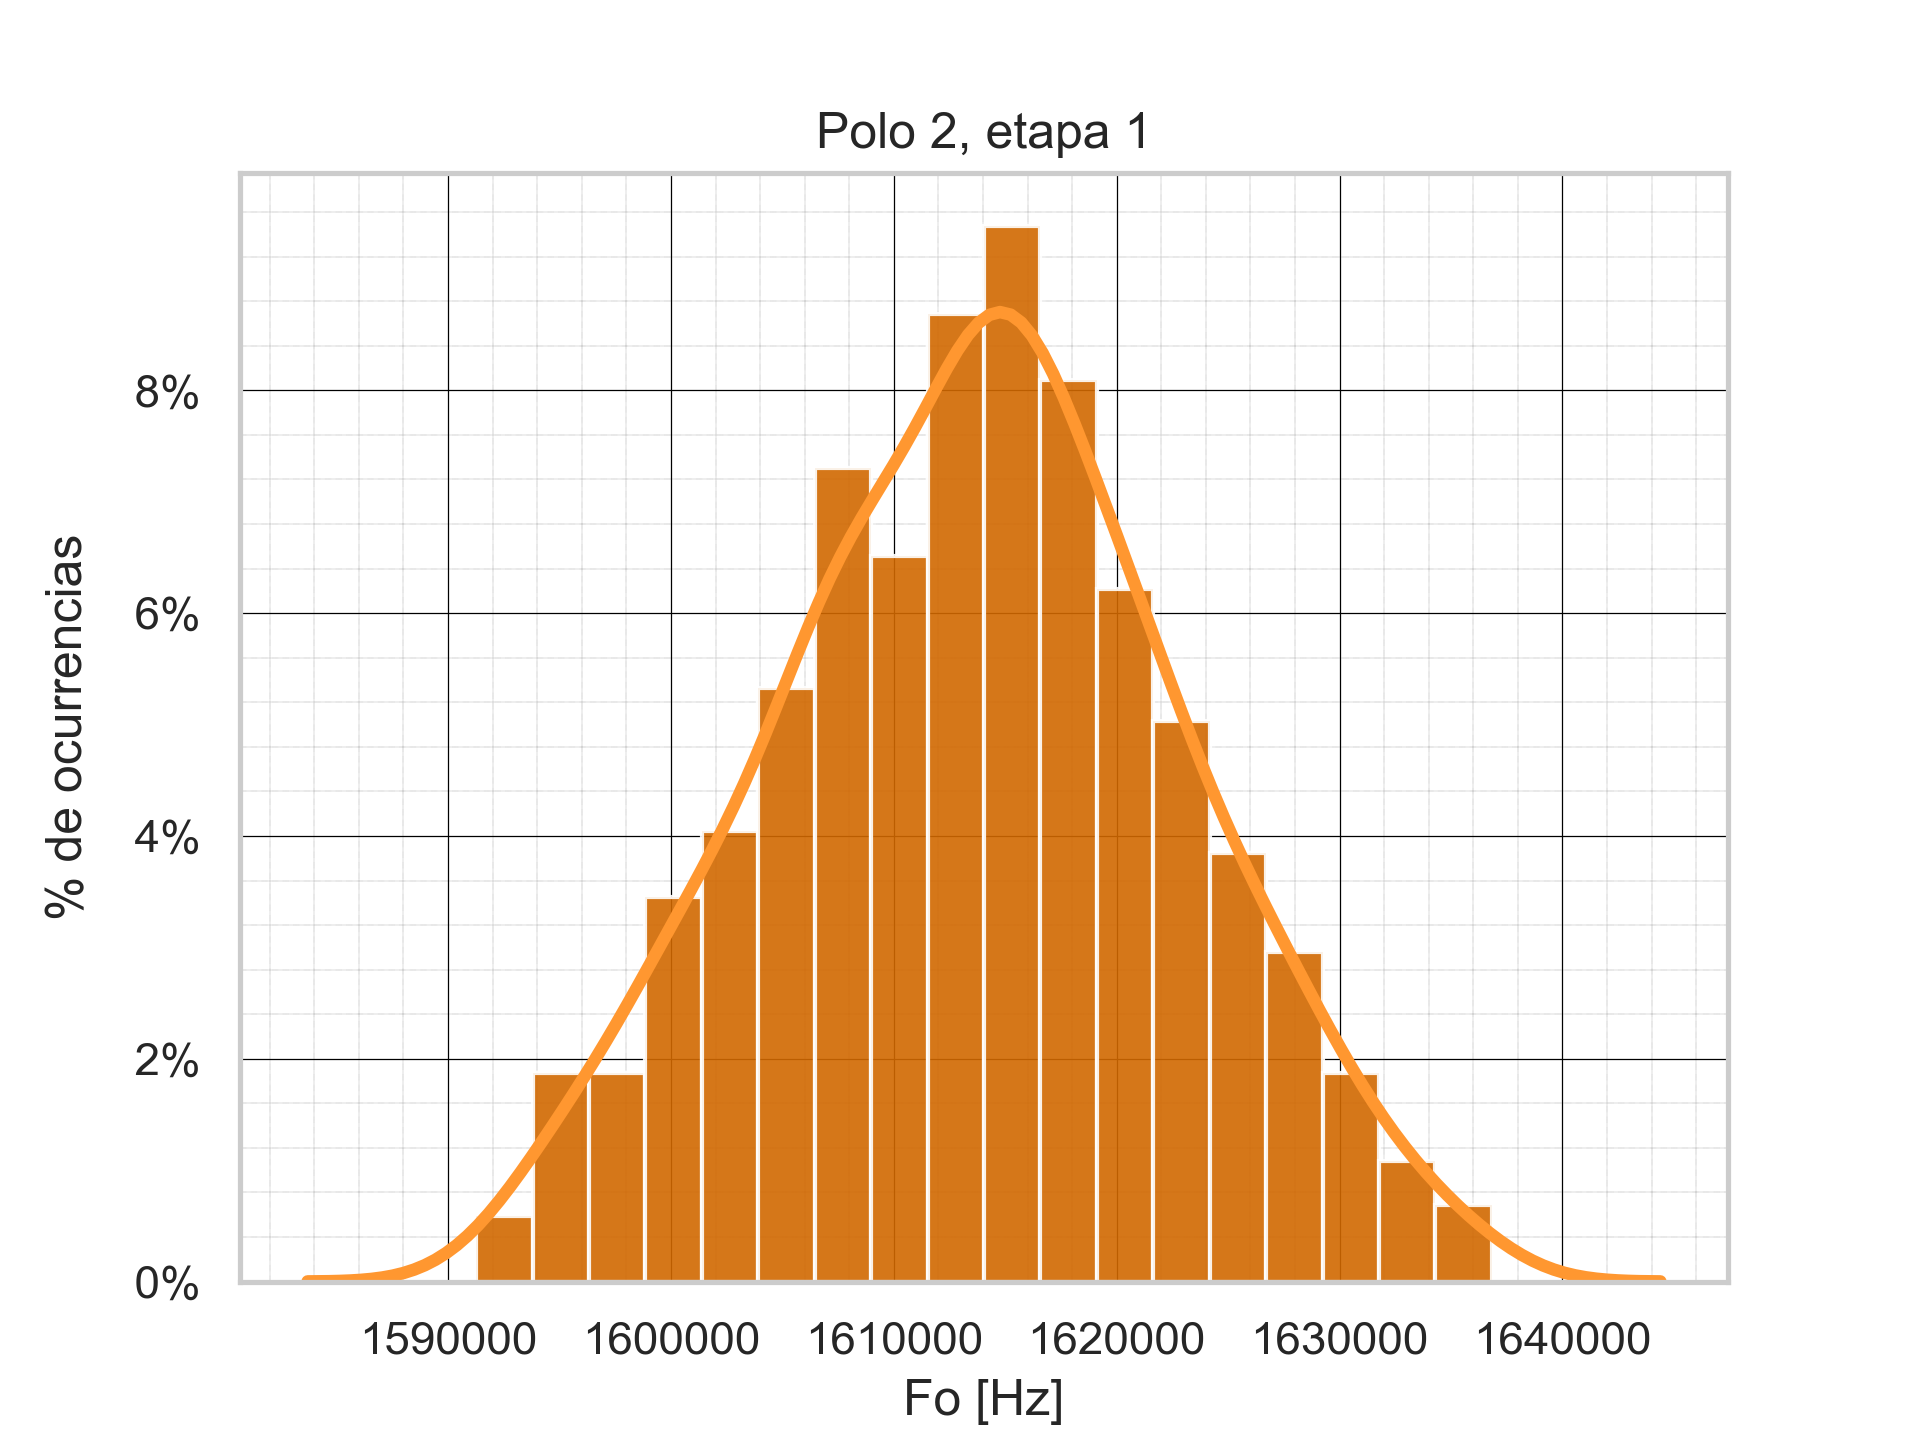
\includegraphics[width=0.45\textwidth]{../Ex3/Resources/histograma_w0_poles_10.png}
    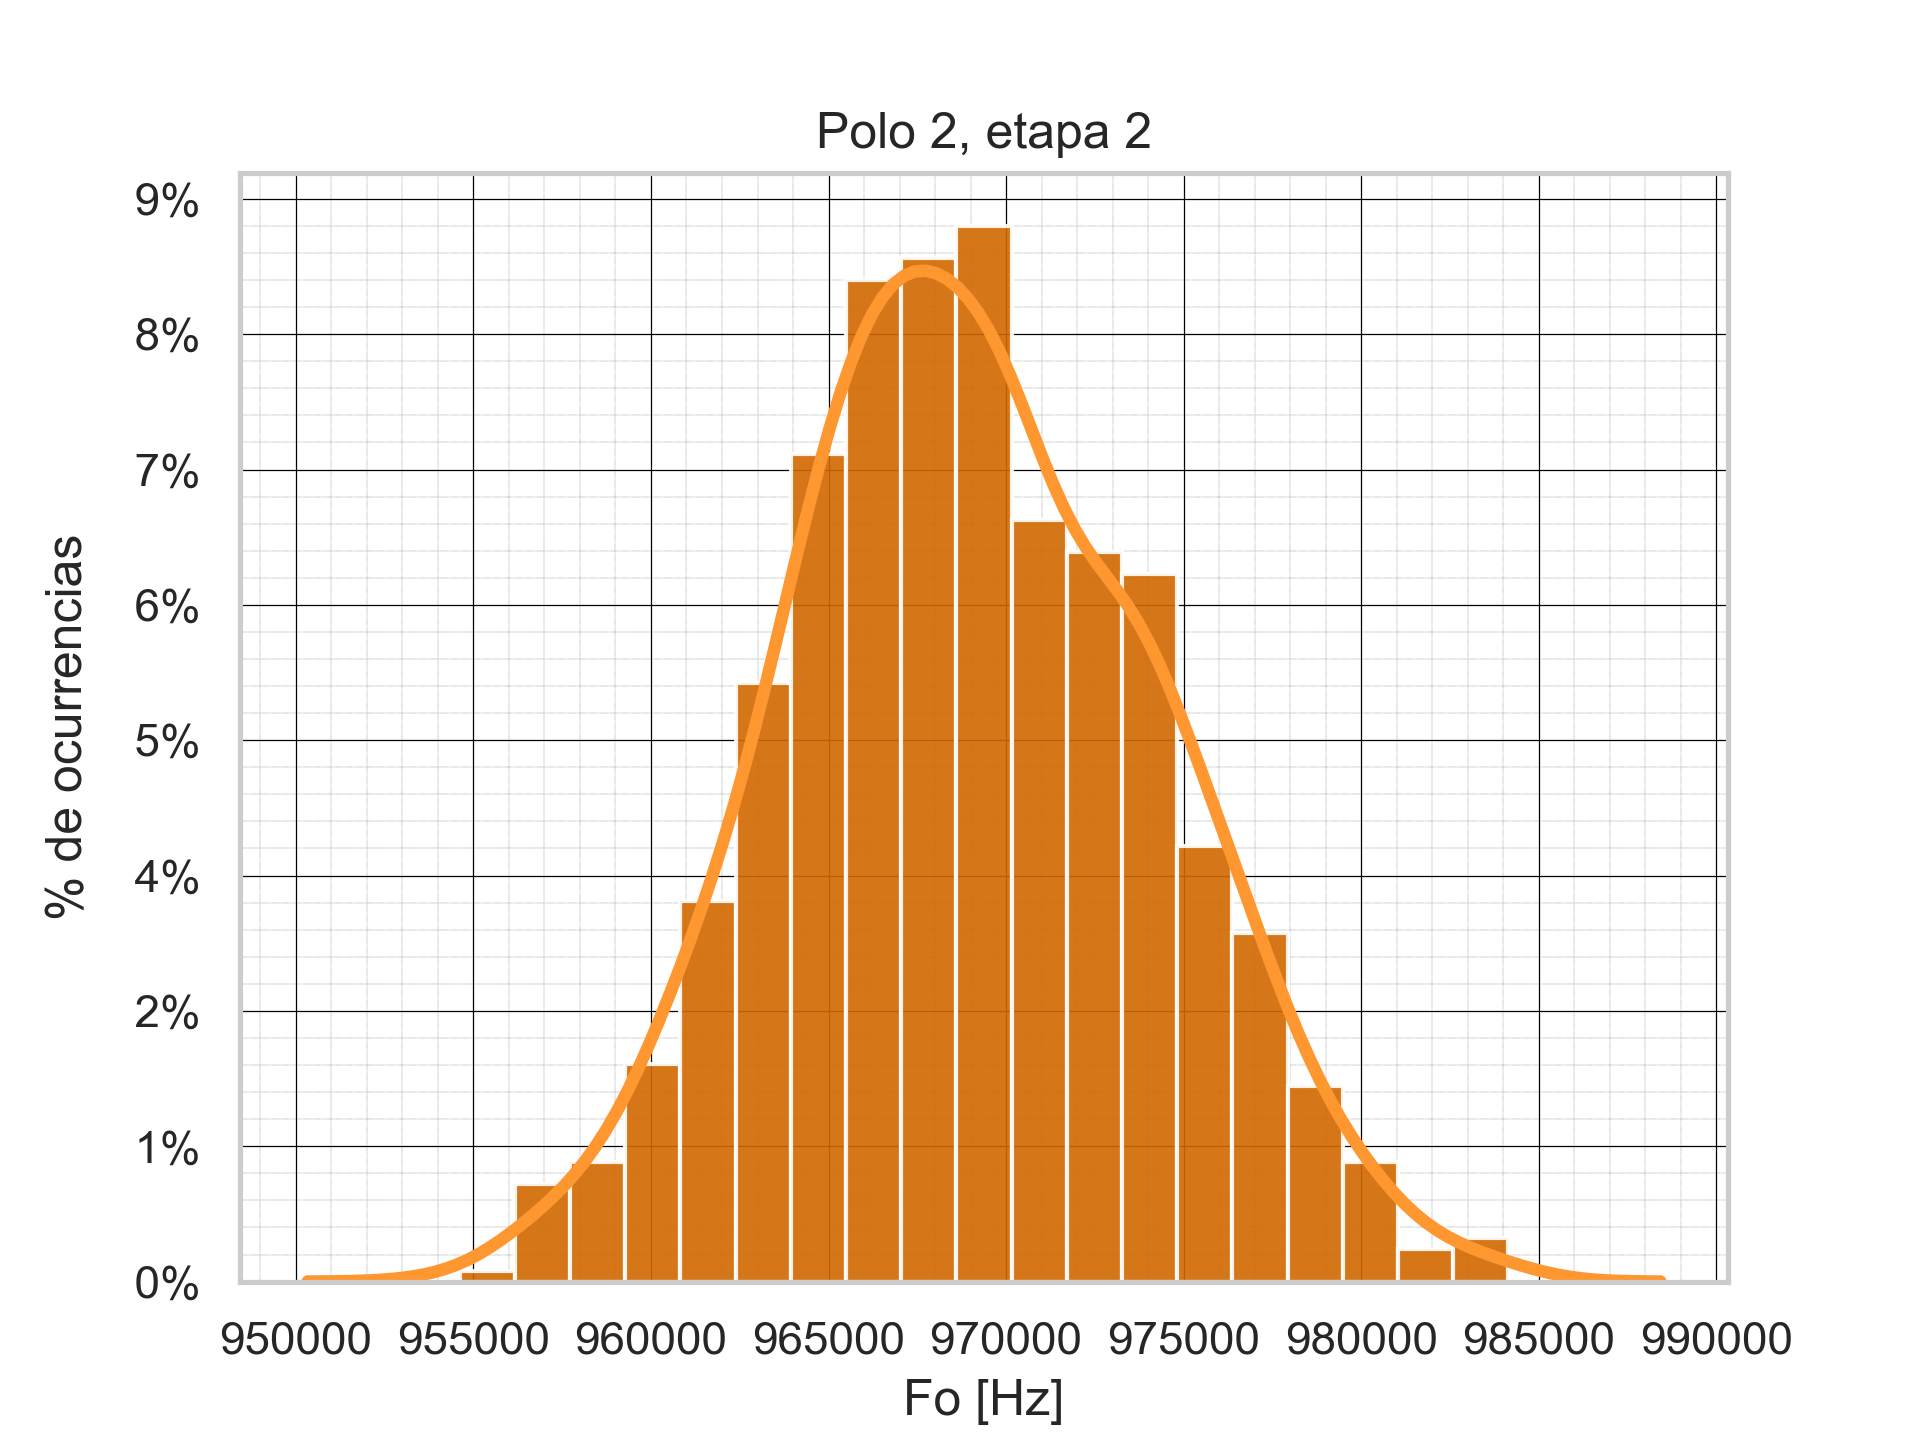
\includegraphics[width=0.45\textwidth]{../Ex3/Resources/histograma_w0_poles_11.png}
    \caption{Histogramas de $f_{0}$ para cada polo}
    \label{sedrahistf0}
\end{figure}
Se puede notar que, para todos los casos, la dispersión de estos parámetros está acotada a un rango del 10-20\%. Se considera que es una dispersión razonable, más habiendo comprobado que para todos los valores tomados el filtro cumple con las especificaciones de la plantilla.

\begin{figure}[H]
    \centering
    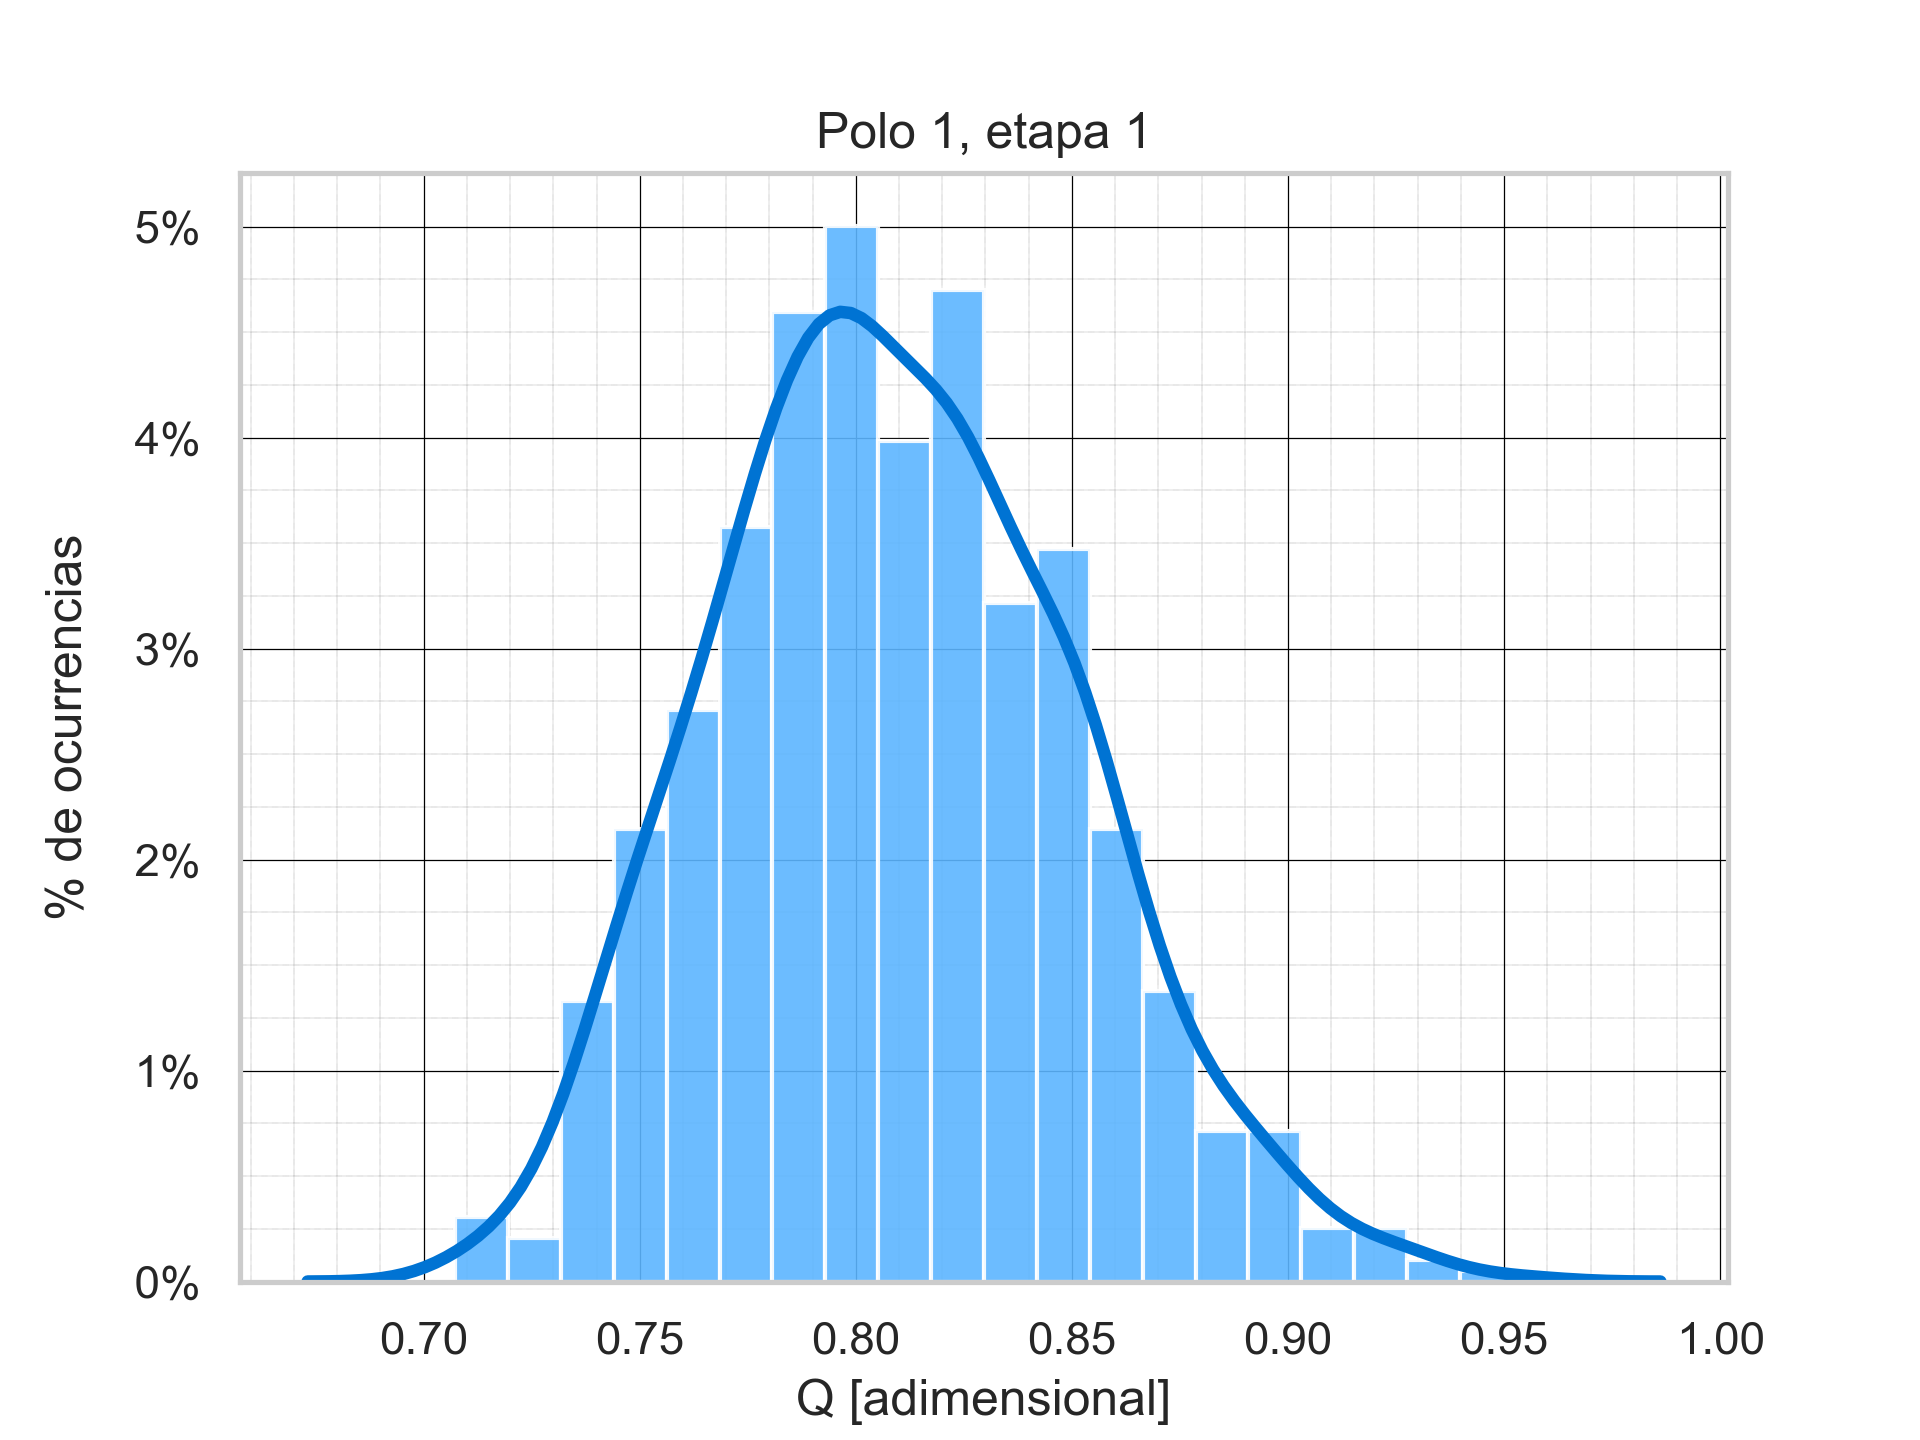
\includegraphics[width=0.45\textwidth]{../Ex3/Resources/histograma_q_poles_00.png}
    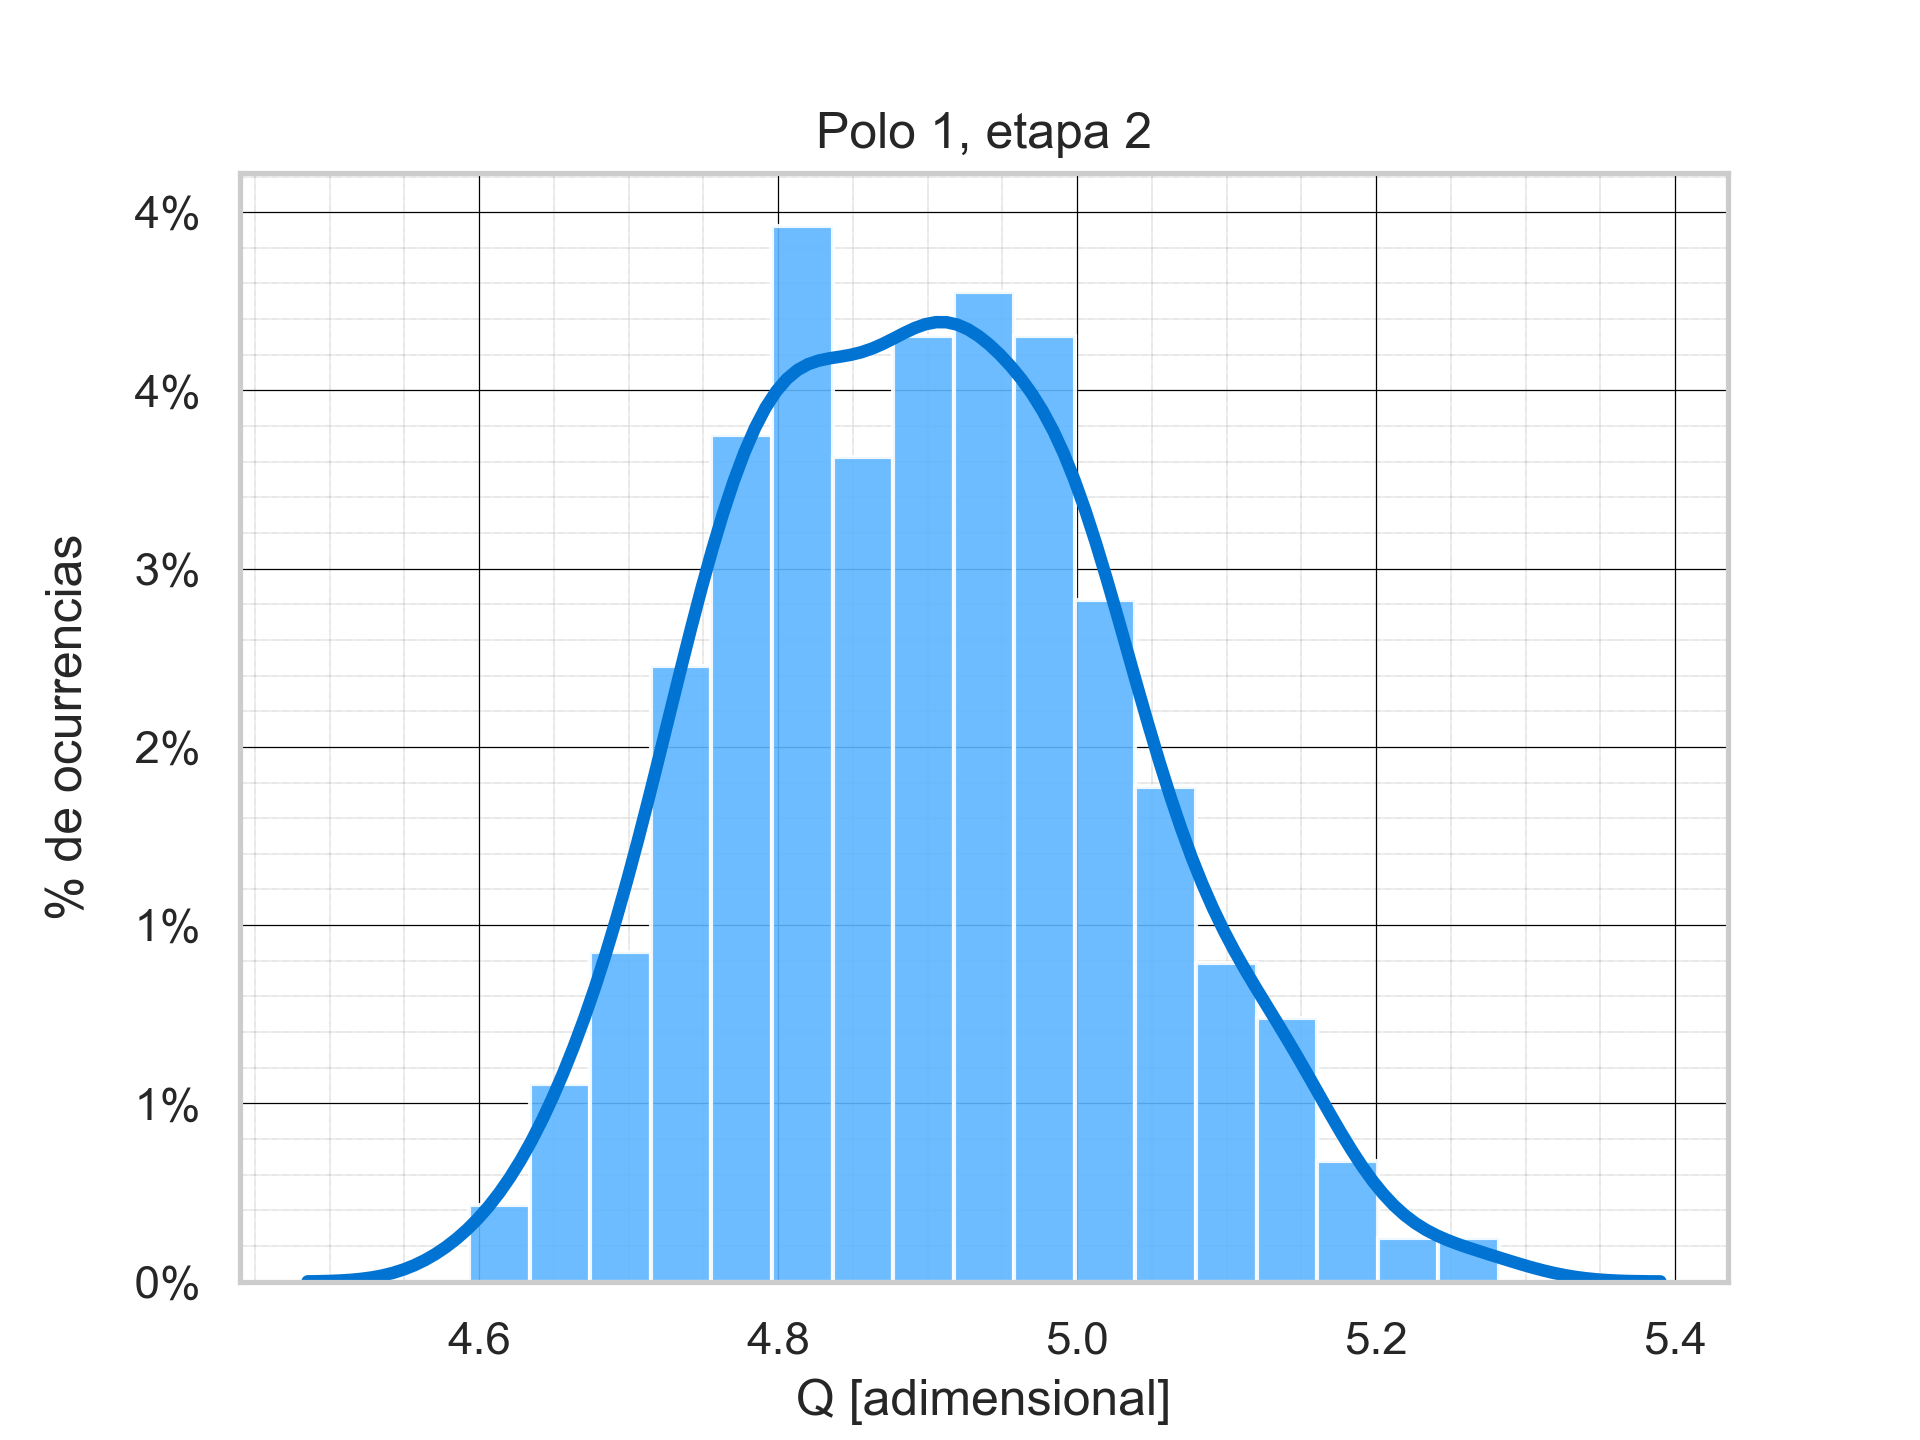
\includegraphics[width=0.45\textwidth]{../Ex3/Resources/histograma_q_poles_01.png}
    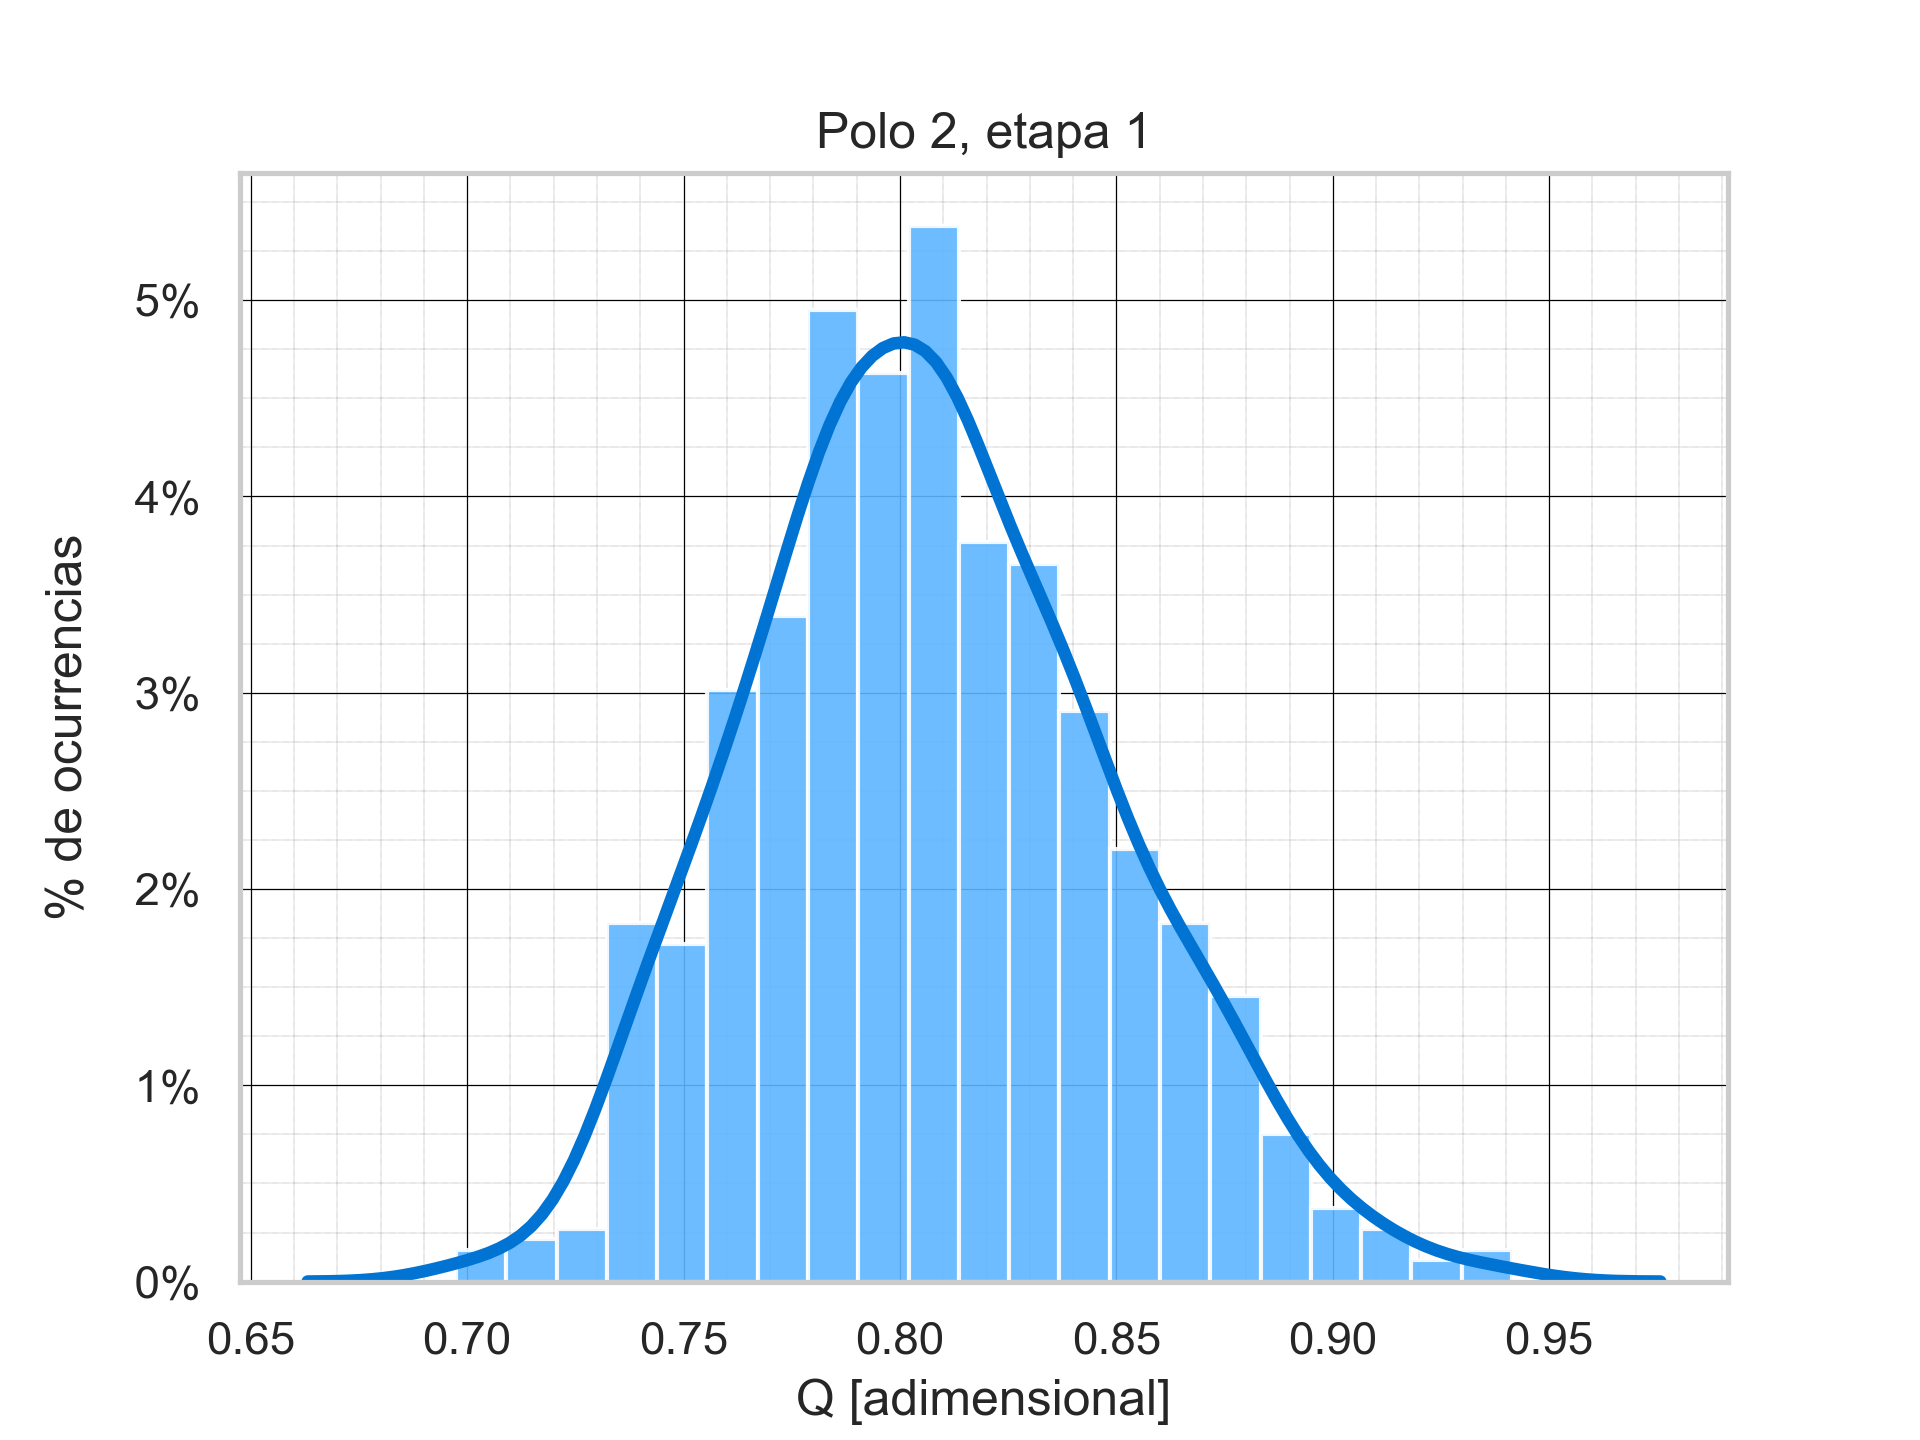
\includegraphics[width=0.45\textwidth]{../Ex3/Resources/histograma_q_poles_10.png}
    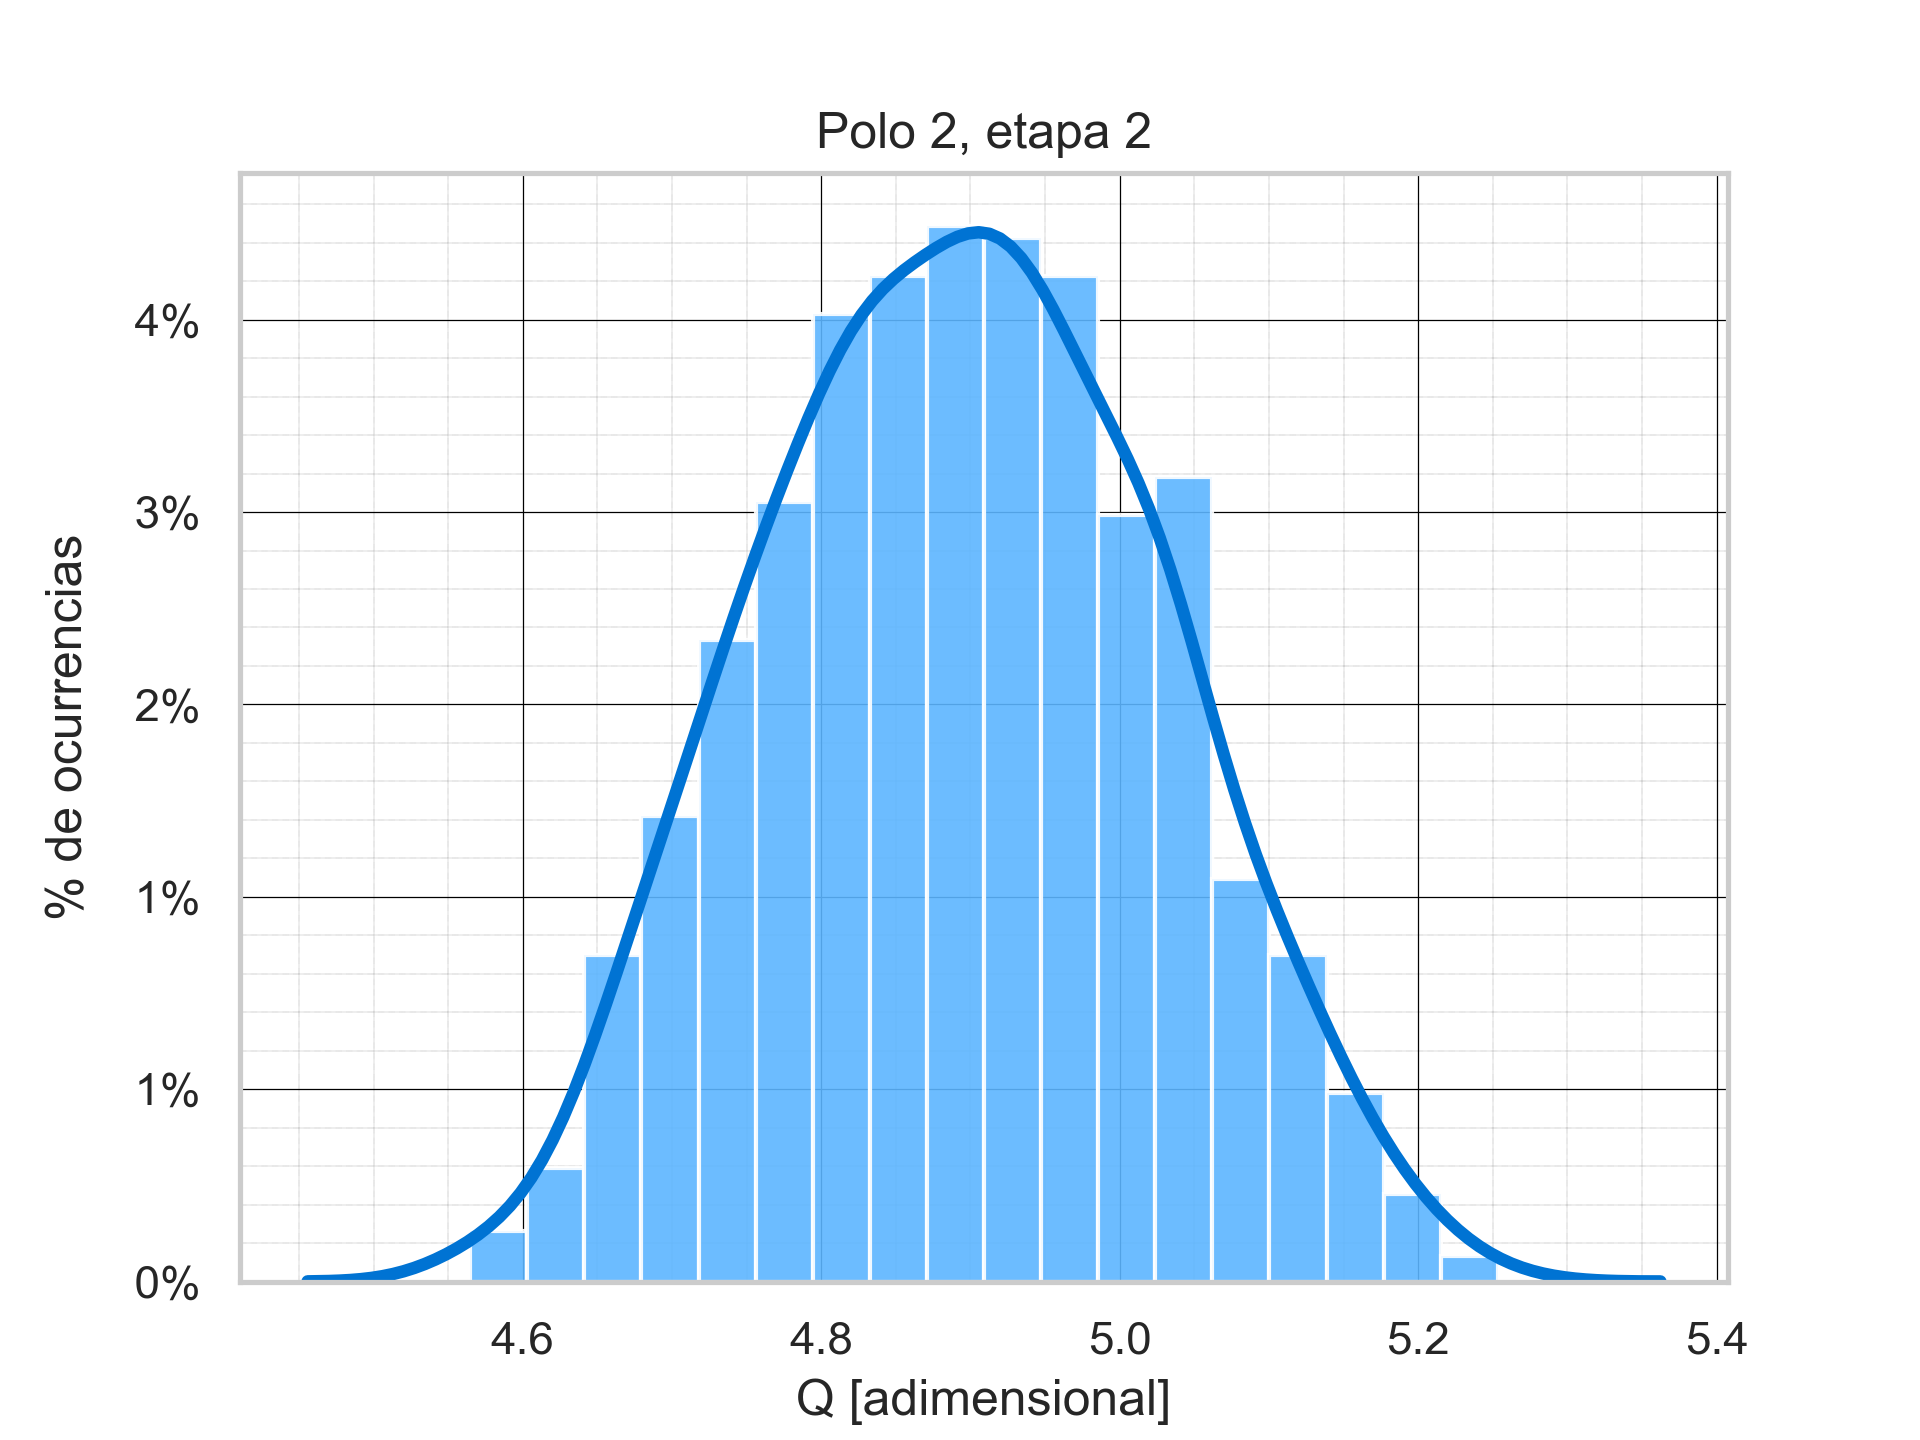
\includegraphics[width=0.45\textwidth]{../Ex3/Resources/histograma_q_poles_11.png}
    \caption{Histogramas de $Q$ para cada polo}
    \label{sedrahistq}
\end{figure}


\subsubsection{Regulación del Q: \emph{presets}}
Se incorporaron al circuito dos resistencias variables (\emph{presets}), una en cada etapa. Estas resistencias se colocaron en lugar de Rb, ya que $\omega_{0}$ es insensible a los cambios en ella. Las sensibilidades de Q y $\omega_{0}$ a las distintas resistencias de cada etapa se pueden obtener del Cuadro \ref{sensibilidades}.

\begin{table}[H]
\begin{centering}
\begin{tabular}{|c|c|c|}
\hline 
 & $\omega_{0}$ & $Q$\tabularnewline
\hline 
$R_{1}$ & -$\frac{1}{2}$ & -($\frac{Q}{Q_{0}}$-$\frac{1}{2}$)\tabularnewline
\hline 
$C_{2}$ & -$\frac{1}{2}$ & -$\frac{1}{2}(\frac{Q}{Q_{0}}-1)$\tabularnewline
\hline 
$C_{3}$ & -$\frac{1}{2}$ & $\frac{1}{2}(\frac{Q}{Q_{0}}-1)$\tabularnewline
\hline 
$R_{4}$ & -$\frac{1}{2}$ & $\frac{Q}{Q_{0}}-\frac{1}{2}$\tabularnewline
\hline 
$R_{a}$ & 0 & $-(\frac{Q}{Q_{0}}-1)$\tabularnewline
\hline 
$R_{b}$ & 0 & $\frac{Q}{Q_{0}}-1$\tabularnewline
\hline 
\end{tabular}
\par\end{centering}
\label{sensibilidades}
\caption{Sensibilidades de $\omega_{0}$ y $Q$ respecto de los componentes
pasivos}
\end{table}

De esta manera, se proporciona una ajuste grueso y uno fino del Q del circuito. La transferencia para distintos valores de estos resistores se simuló y se puede observar en la Figura \ref{ambospreset}.
\begin{figure}[H]
    \centering
    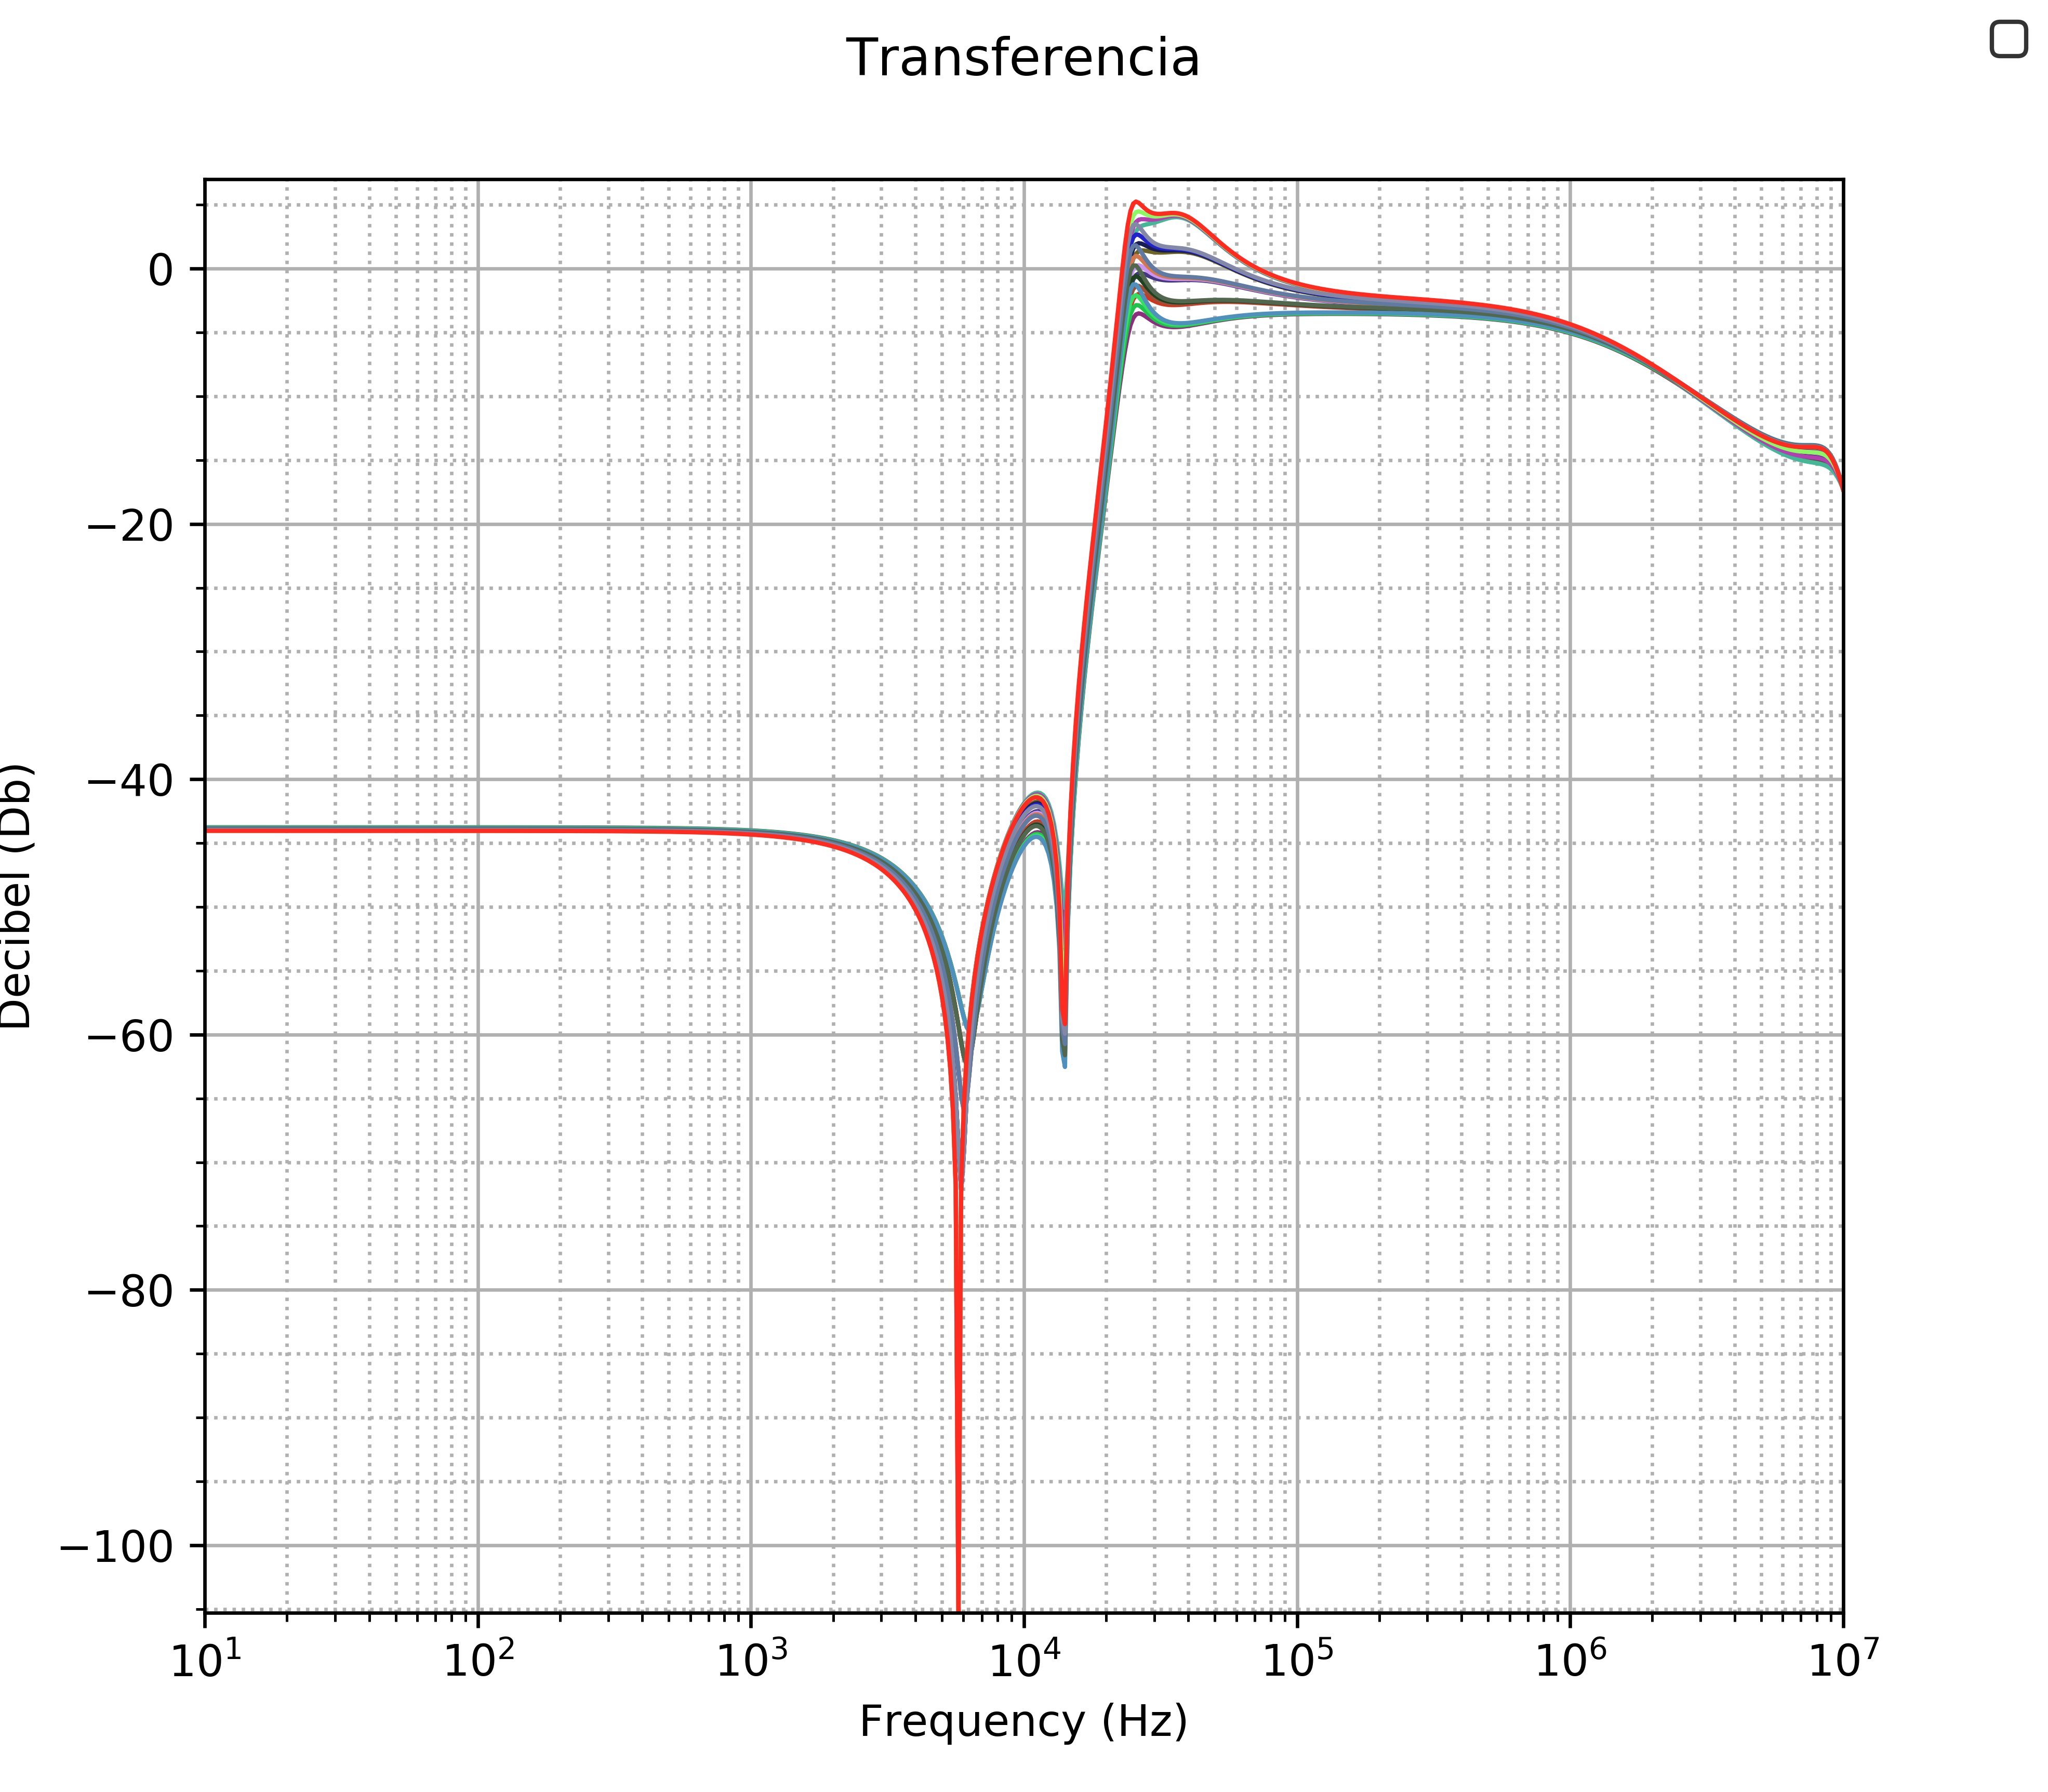
\includegraphics[width=0.6\textwidth]{../Ex3/Resources/ambospreset.png}
    \caption{Efectos de las resistencias variables sobre la transferencia del circuito}
    \label{ambospreset}
\end{figure}

\subsubsection{Estabilidad: respuesta a una señal cuadrada}
Se simuló la respuesta a una señal cuadrada del circuito completo, y como se ve en la Figura \ref{medicrespesc}, el sistema se comporta de forma deseable: la oscilación del transitorio se estabiliza en medio período para frecuencias de hasta MHz.


\section{Mediciones}
Se implementó el circuito completo, que se muestra en la Figura \ref{circuitocompleto}, en PCB. Todas las resistencias utilizadas son de montaje superficial con tolerancias del 1\% y  los capacitores tienen una tolerancia del 10\%. Los integrados utilizados para la implementación del filtro en principio estaba pensado que fueran del tipo LM833, por su generoso BWP de 120kHz, para evitar atenuar buena parte de la banda pasante. Sin embargo, por limitaciones de disponibilidad, se utilizó el modelo TL082. Se muestran las simulaciones para ambos. El integrado para el \emph{buffer} de entrada es TL082, también por restricciones de disponibilidad.

\begin{figure}[H]
    \centering
    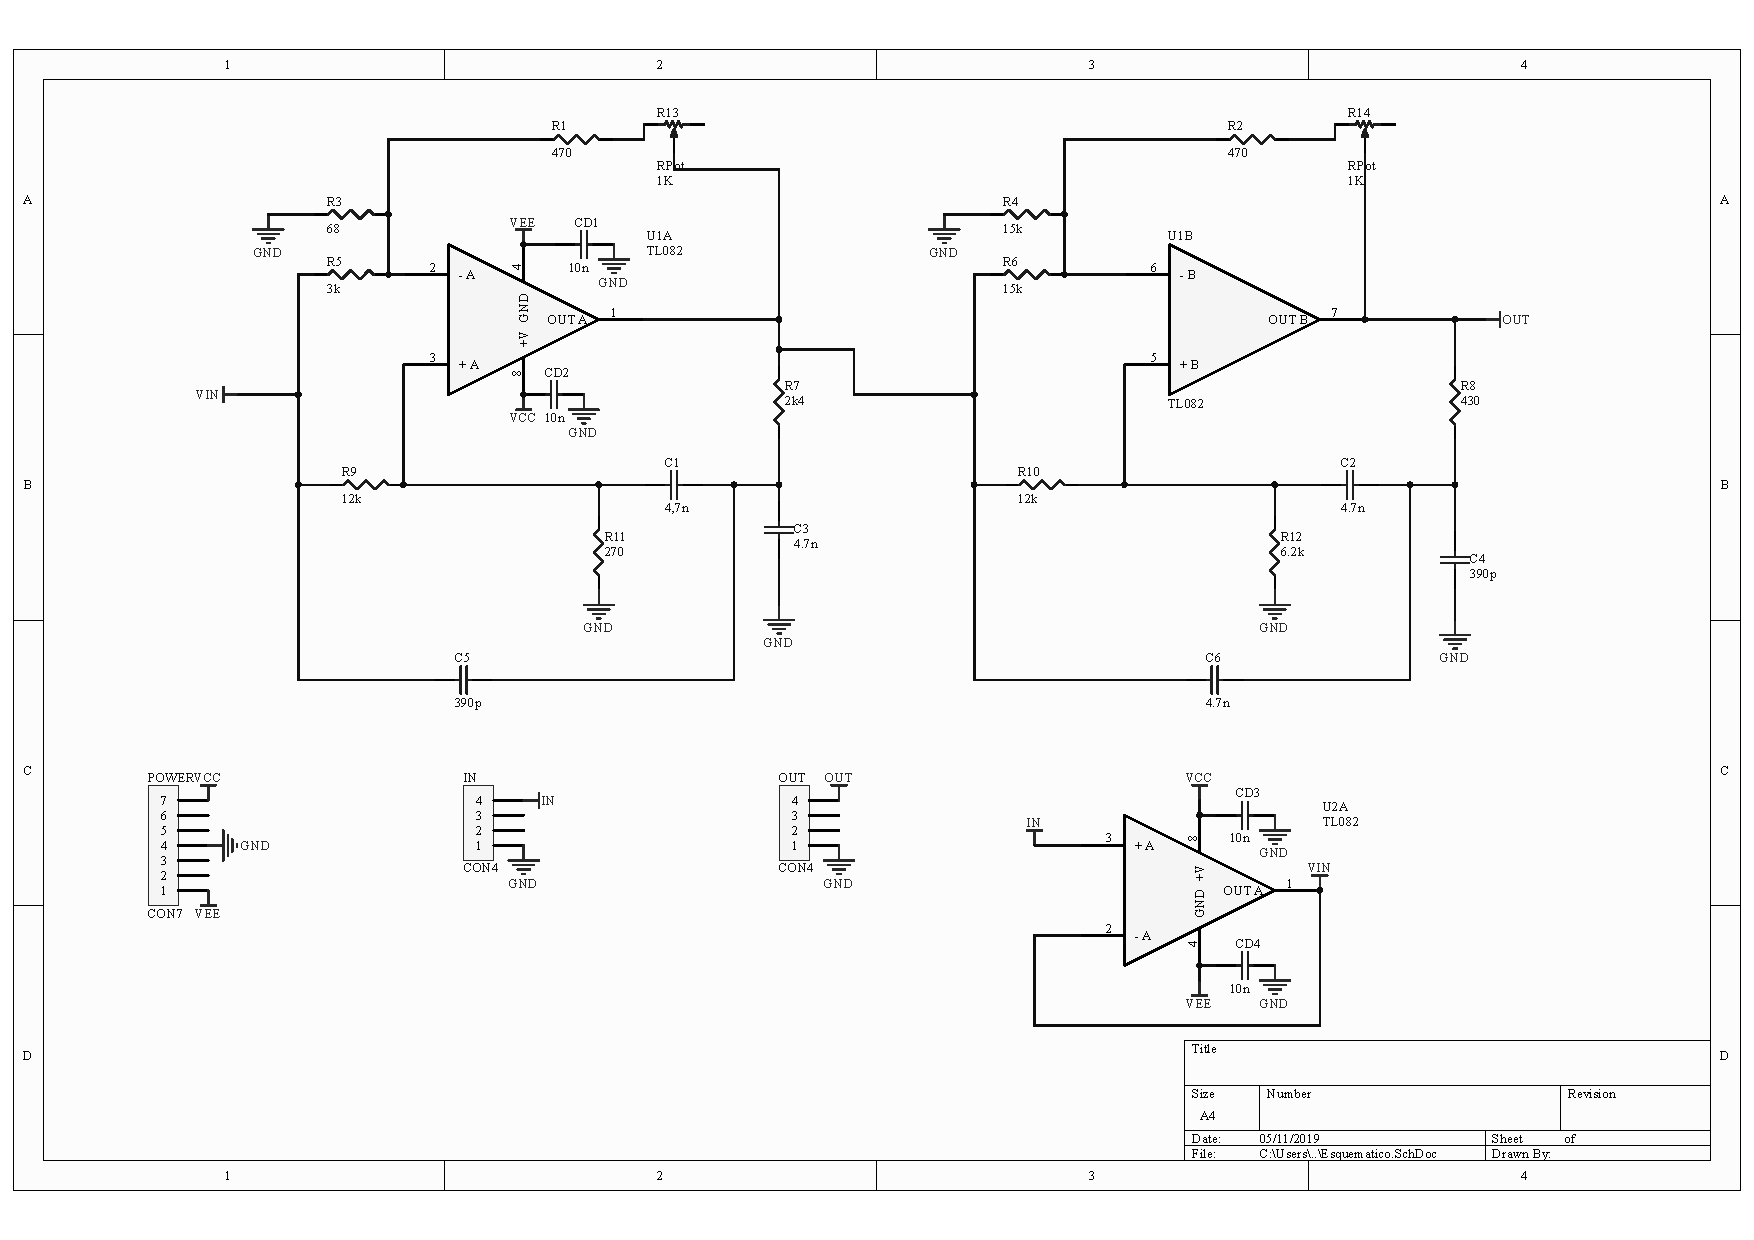
\includegraphics[angle=90,origin=c,width=0.8\textwidth]{../Ex3/Resources/Esquematico.pdf}
    \caption{Circuito completo implementado en PCB}
    \label{circuitocompleto}
\end{figure}

A continuación, se realiza una comparación de los valores relevantes ya examinados en secciones anteriores con las mediciones reales realizadas sobre el circuito.

\subsubsection{Respuesta en frecuencia}
La comparación de respuesta en frecuencia teórica, medida sobre el TL082 y simulada para ambos integrados puede observarse en la Figura \ref{medicrespfrec}.

\begin{figure}[H]
    \centering
    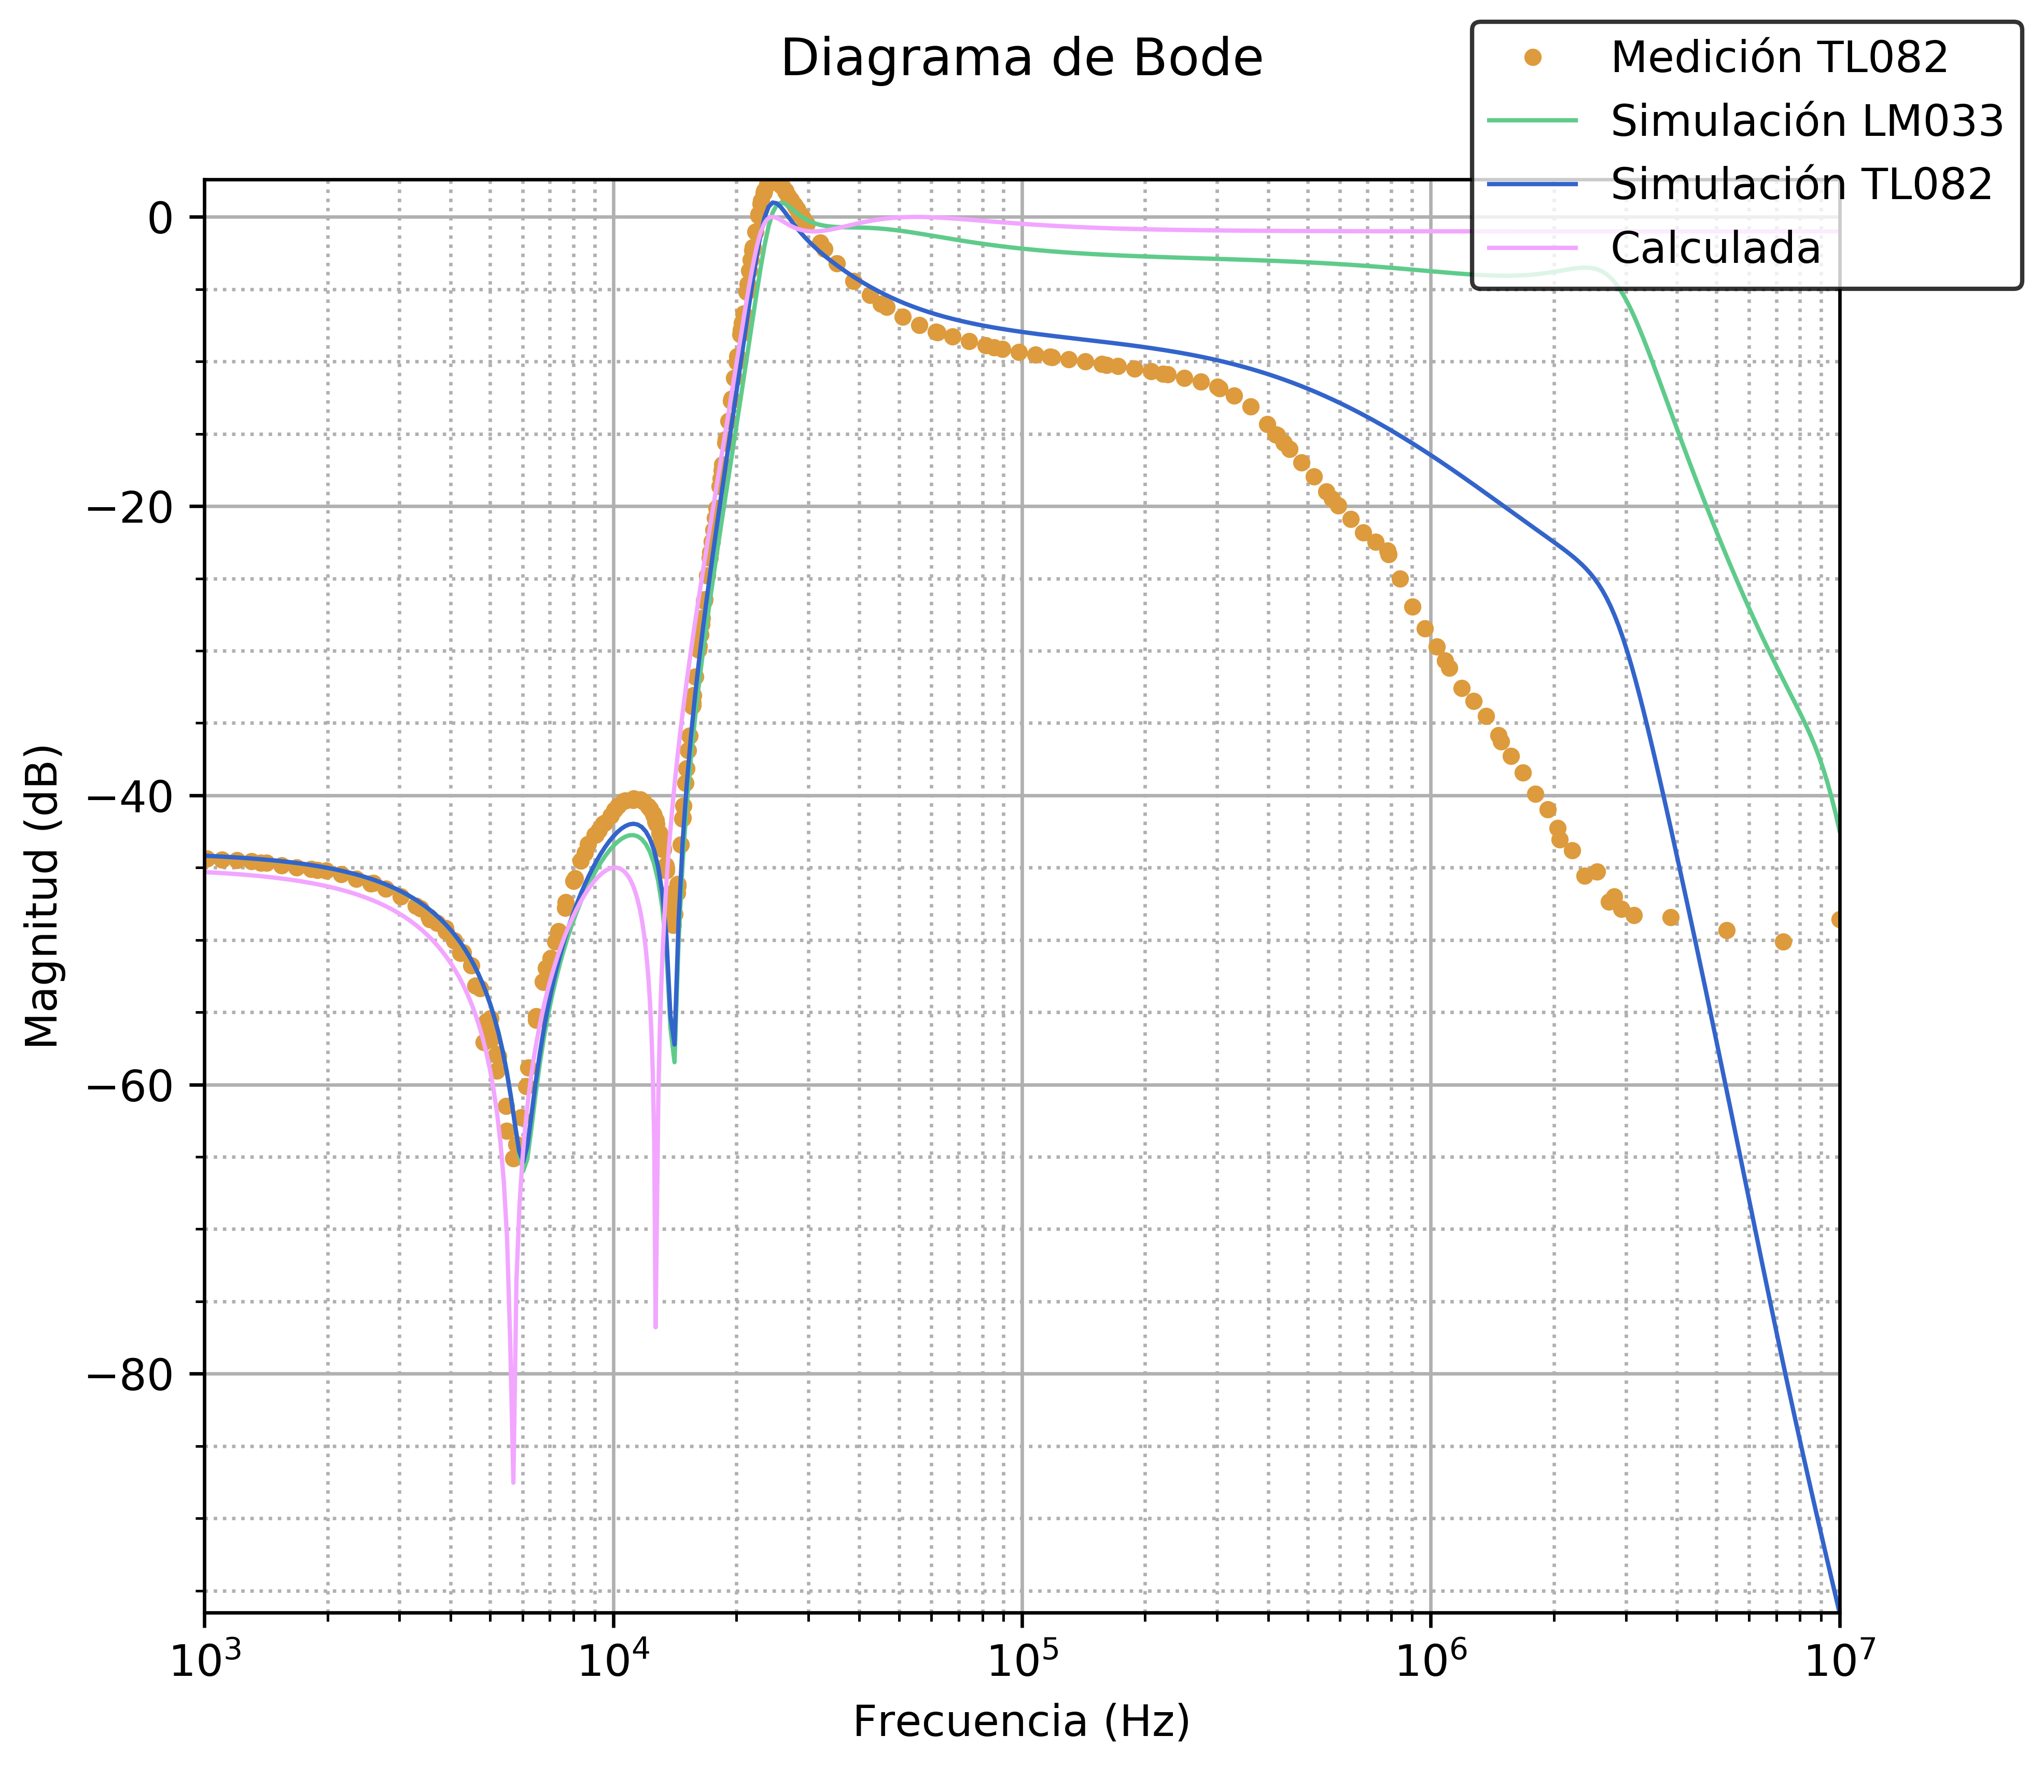
\includegraphics[width=0.7\textwidth]{../Ex3/Resources/medicrespfrec.png}
    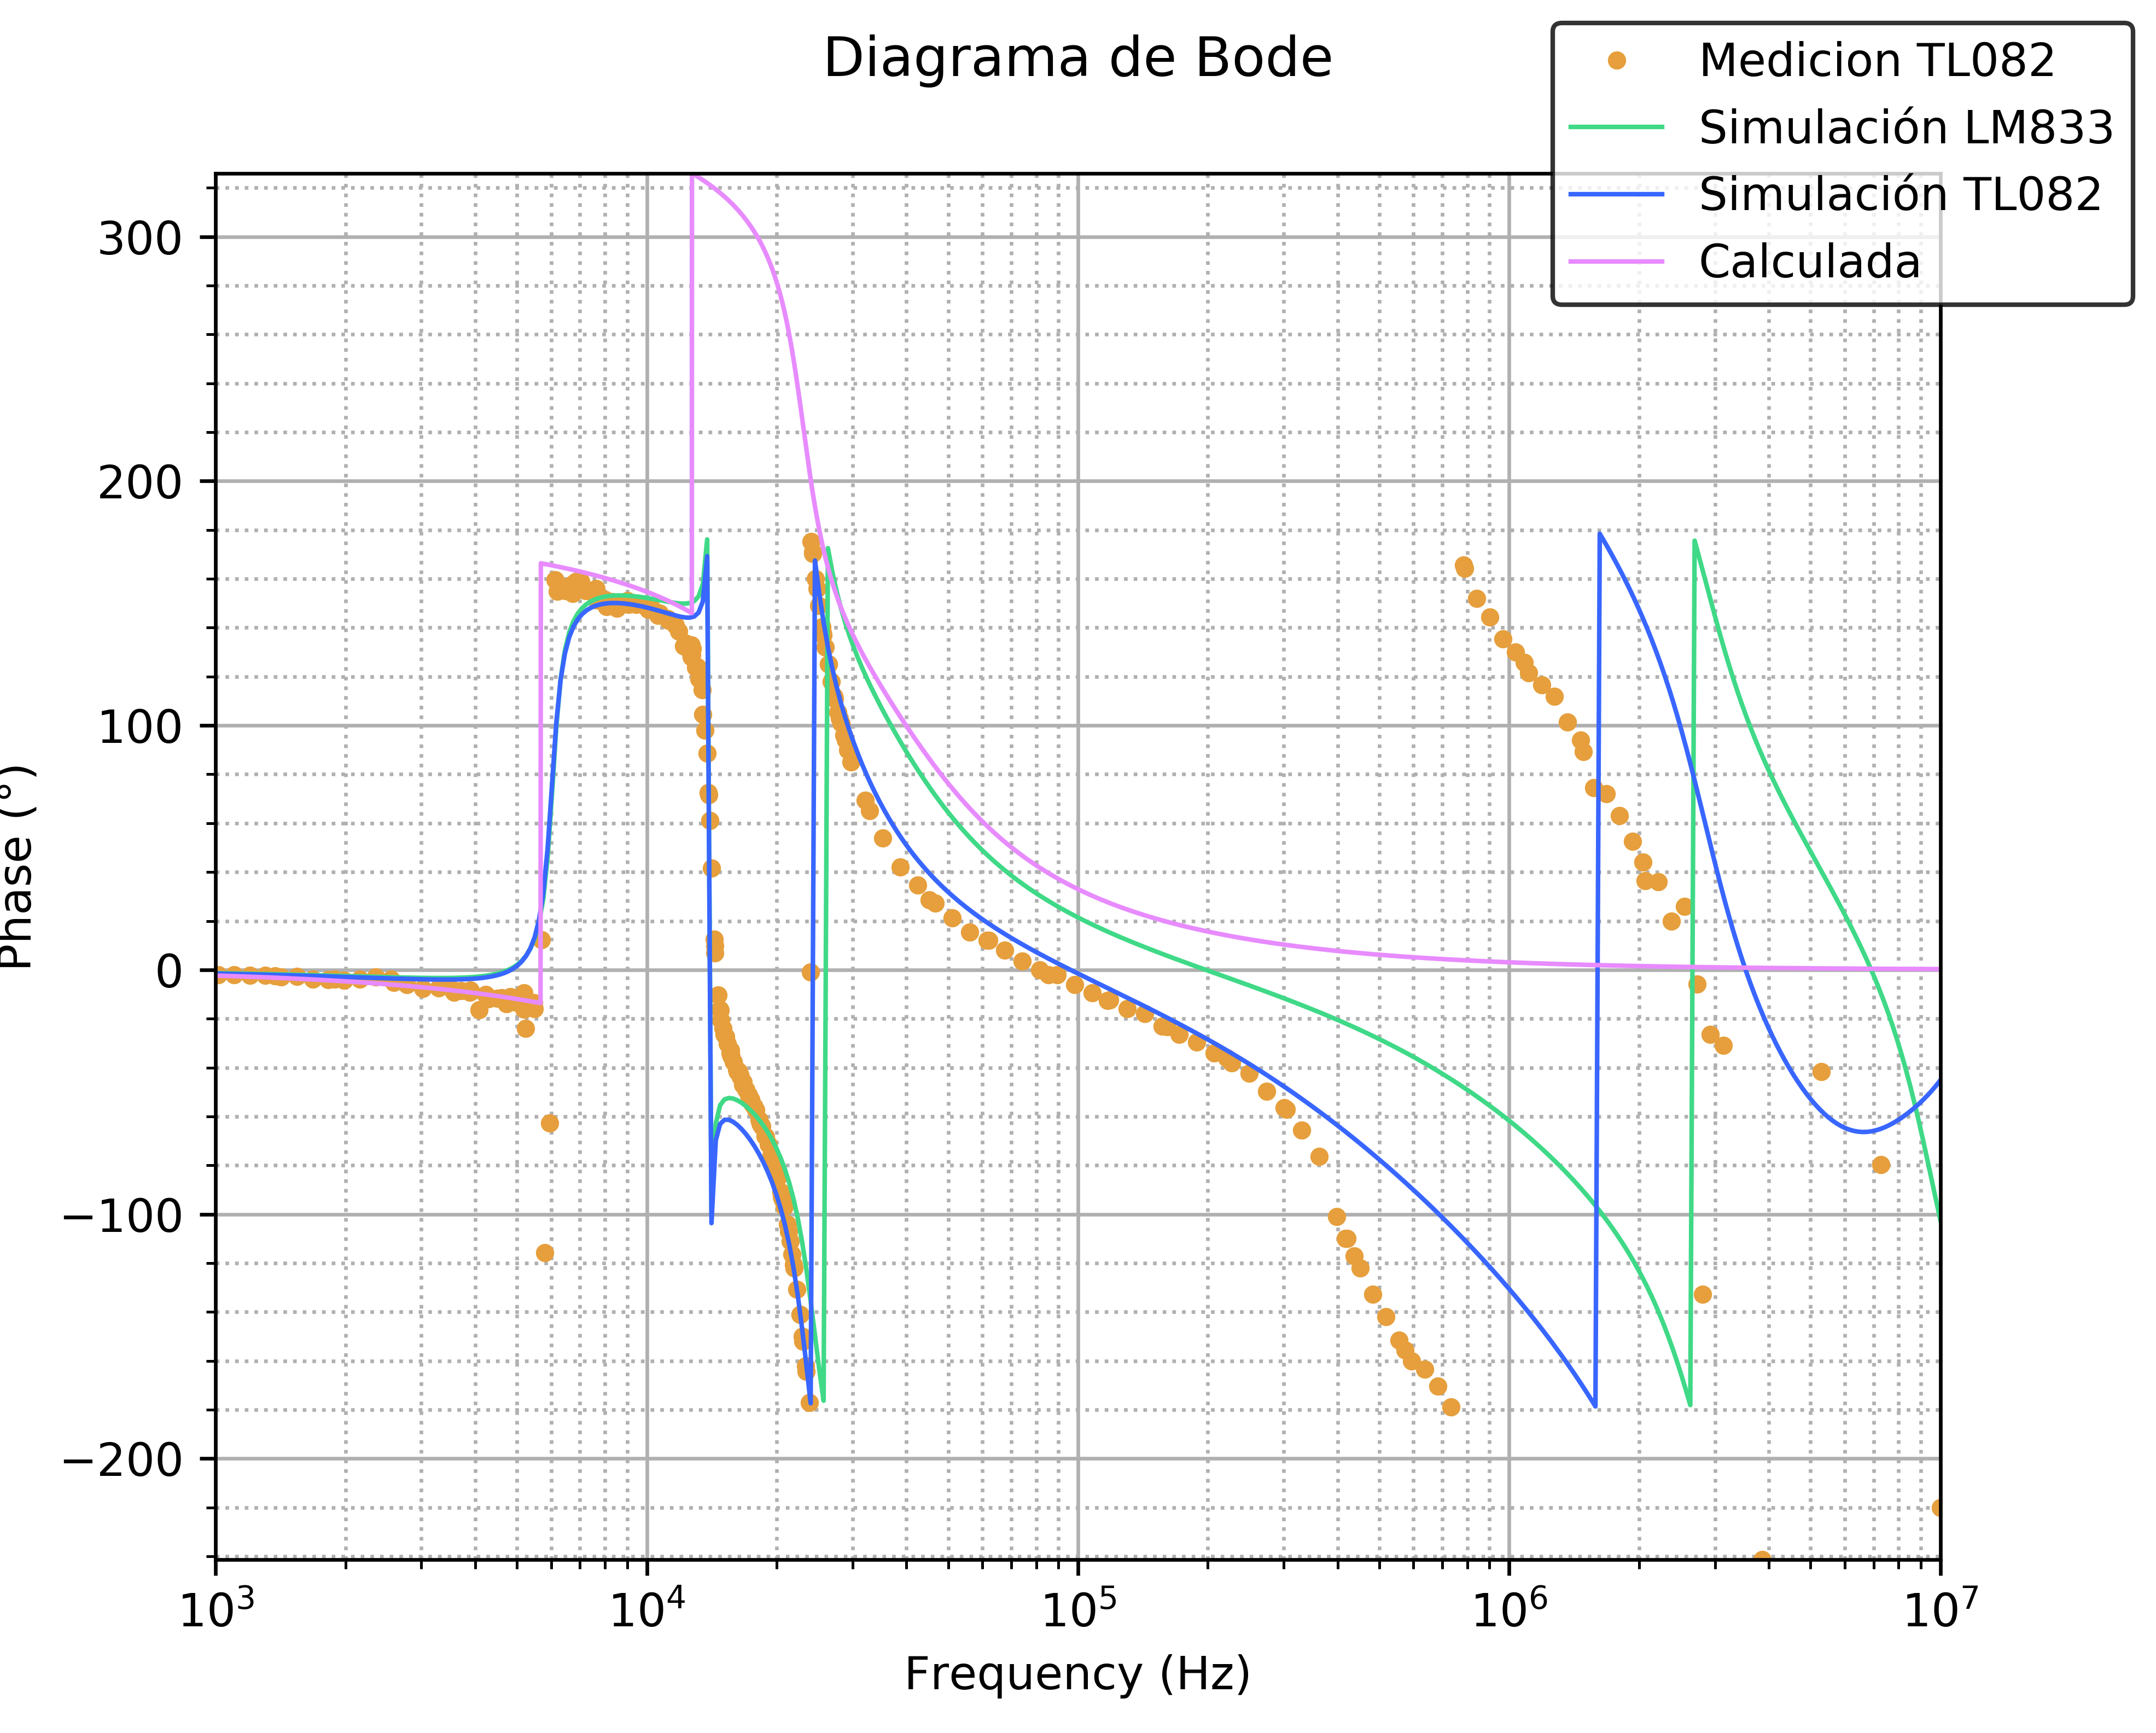
\includegraphics[width=0.7\textwidth]{../Ex3/Resources/medicrespfrecfase.png}
    \caption{Comparación respuesta en frecuencia: teórico, simulado, medido}
    \label{medicrespfrec}
\end{figure}

Se observó que los resultados medidos fueron muy similares a los teóricos y simulados. A pesar del muy limitado ancho de banda, se consideró que estos fueron satisfactorios. En el gráfico de fase, se aprecia que para los valores de componentes reales, el cero de la primera etapa mencionado en la sección \ref{transftotalcirc} se ubica del lado derecho del eje imaginario, dando origen al cambio positivo de fase en 5kHz. Esto resulta subóptimo, ya que puede provocar problemas de estabilidad en el circuito.

\subsubsection{Respuesta al escalón}
La comparación de respuesta al escalón medida y simulada puede observarse en la Figura \ref{medicrespesc}.

\begin{figure}[H]
    \centering
    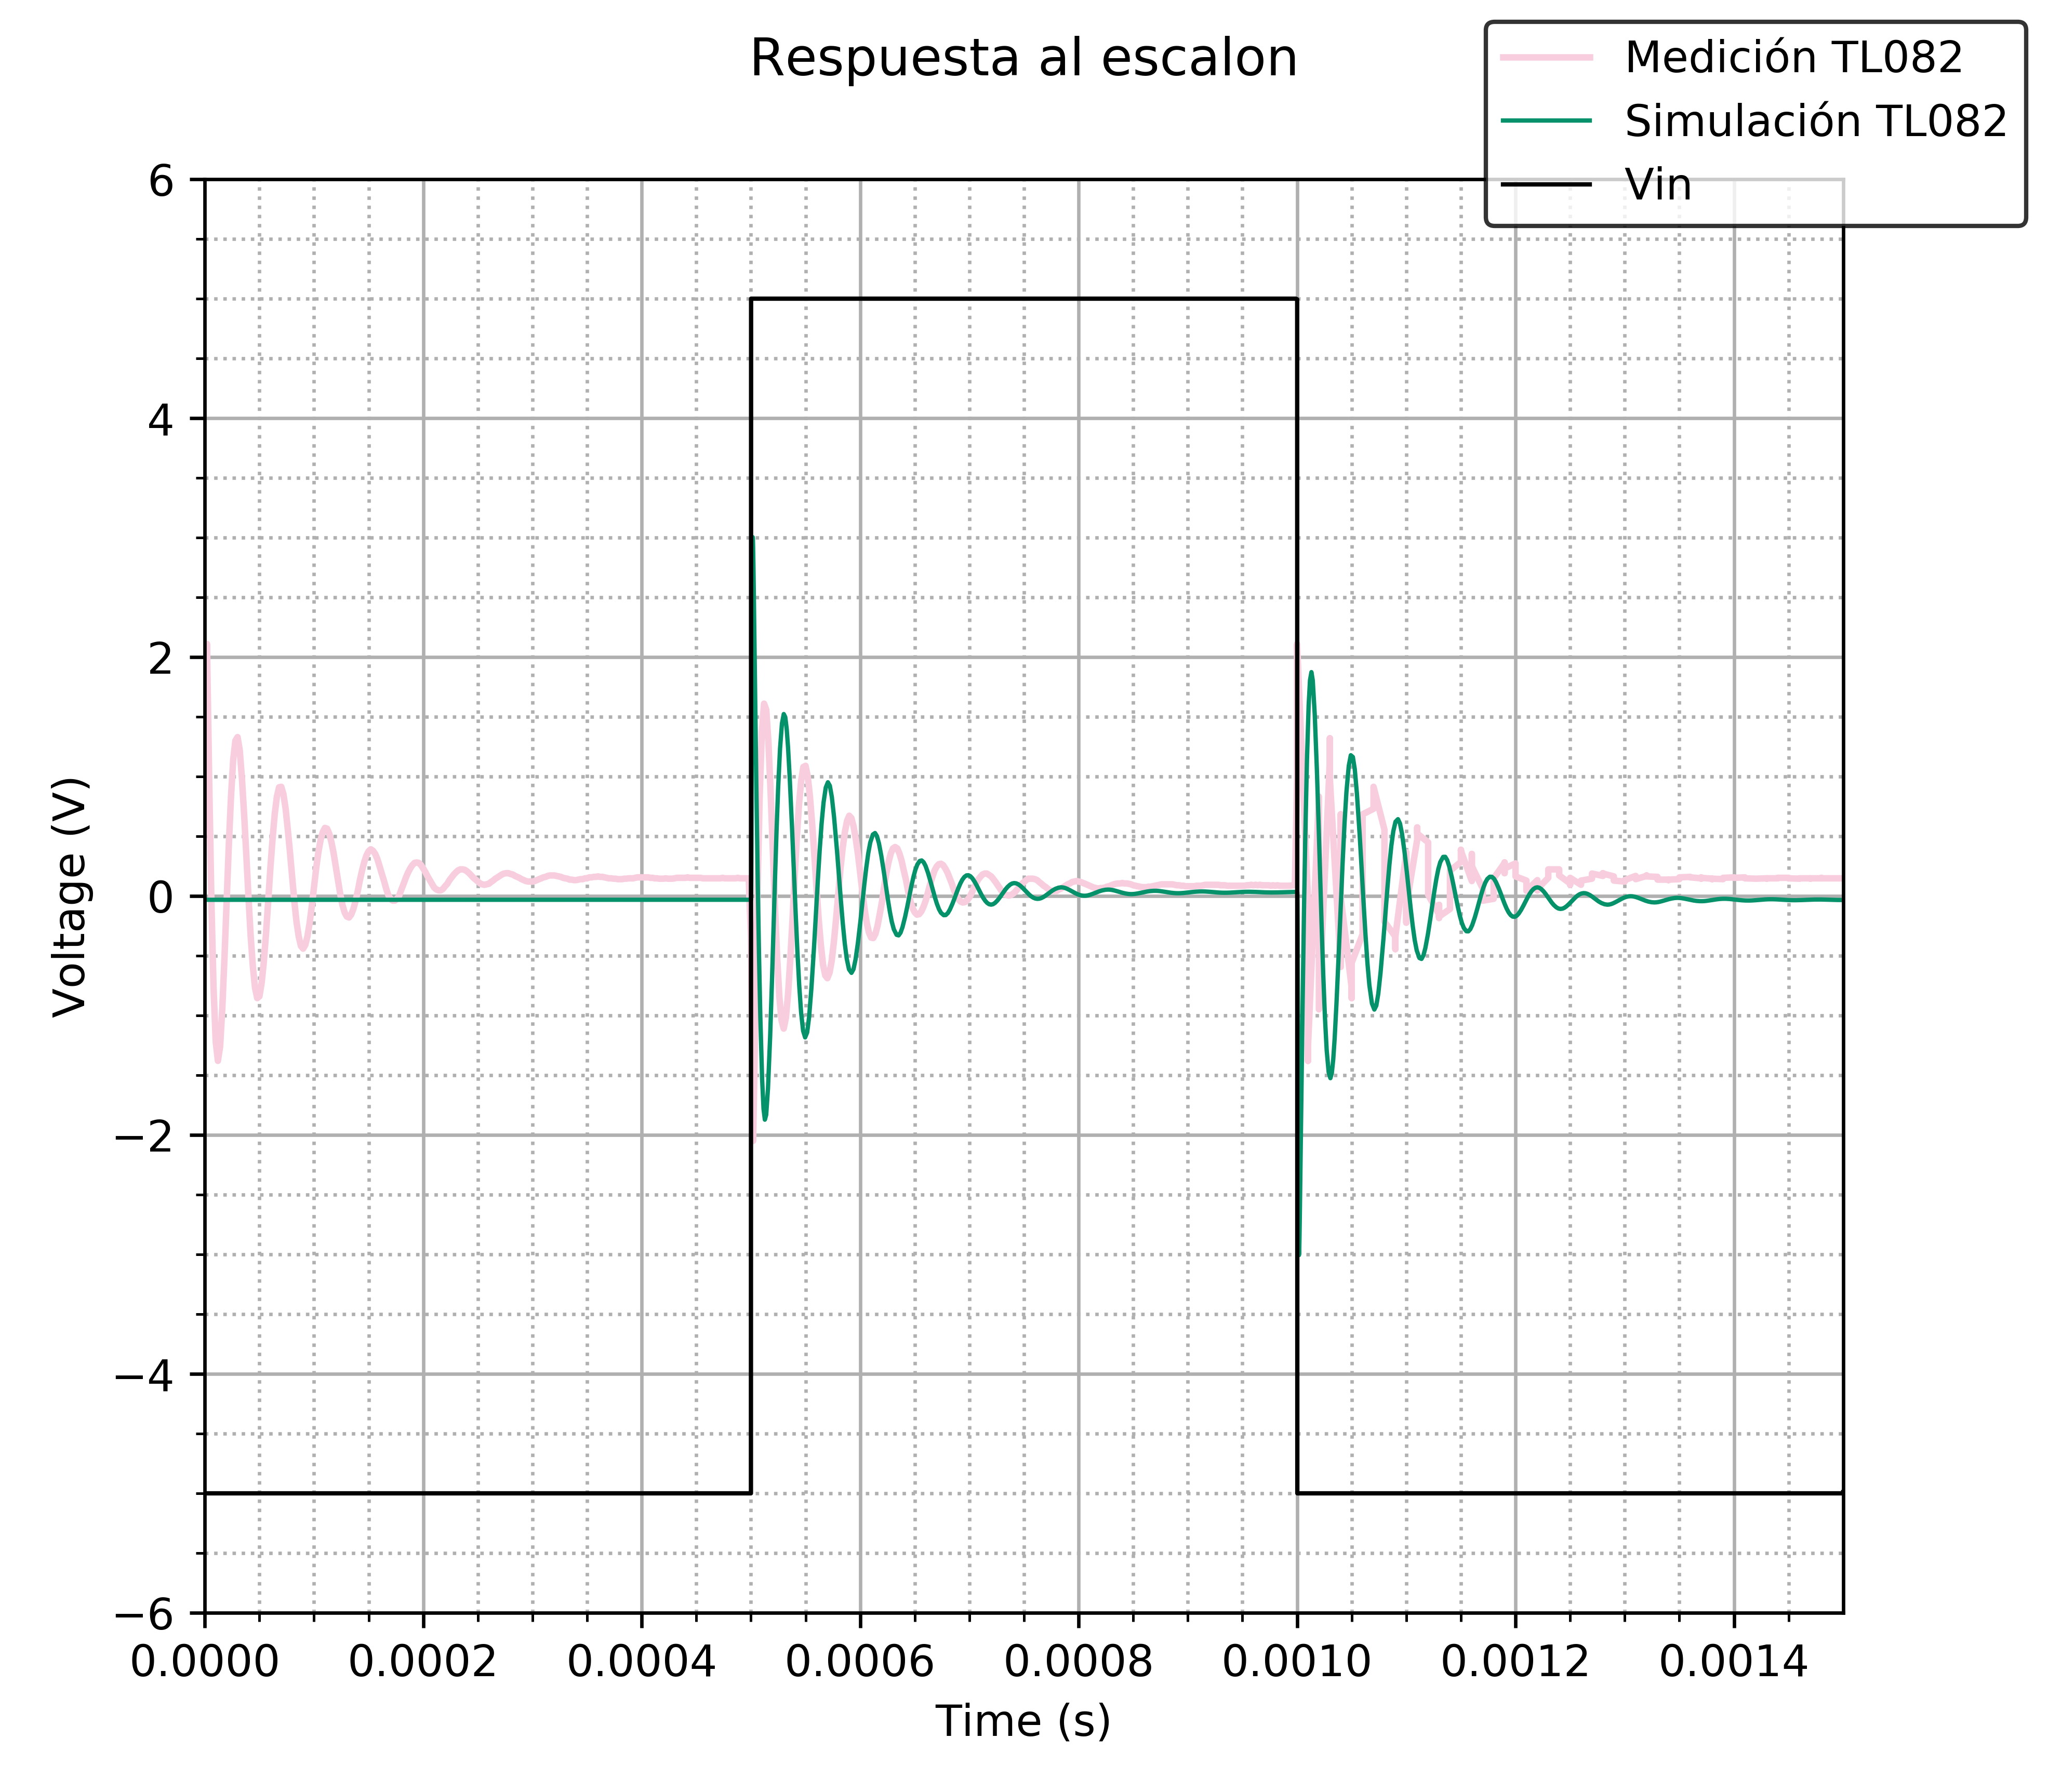
\includegraphics[width=0.7\textwidth]{../Ex3/Resources/medicrespesc.png}
    \caption{Comparación respuesta al escalón: teórico, simulado, medido}
    \label{medicrespesc}
\end{figure}

Se observa que el circuito no oscila, no tiene problemas de estabilidad, confirmando el estudio previo a la construcción del circuito. Los resultados son satisfactorios.

\section{Conclusión}
Se implementó existosamente un filtro pasa-altos haciendo uso de las mejoras propuestas por Sedra, Ghorab y Martin al circuito de Deliyannis-Friend. Este filtro tiene similares sensibilidades para los polos, pero reducidas para los ceros de transmisión. Aprovechando las facilidades provistas por los autores, se pudo realizar un filtro que cumple una plantilla considerablemente restrictiva economizando notablemente en componentes.% habria que darle una manito a esto